\documentclass[12pt]{article}

% Shared HSC style packages (see ../HSC-Common/).
\makeatletter
\def\input@path{{../HSC-Common/styles/}{./}}
\makeatother
\newcommand{\HSCBookletHeaderTitle}{Matrix Practice}

\usepackage{amsmath}
\usepackage{amssymb}
\usepackage{amsthm}
\newtheorem*{theorem}{Theorem}
\usepackage{geometry}
\usepackage[utf8]{inputenc}
% Links without visible rectangles (TOC and cross-refs remain clickable).
\usepackage[hidelinks]{hyperref}
\hypersetup{hidelinks}
\usepackage{graphicx}
\usepackage{enumitem}
\usepackage{tikz}
\usetikzlibrary{calc}
\usepackage{nicematrix} % Useful for drawing matrices with blocks/labels
\usepackage{blkarray}   % Useful for block arrays

\usepackage{listings}
\definecolor{codegreen}{rgb}{0,0.6,0}
\definecolor{codegray}{rgb}{0.5,0.5,0.5}
\definecolor{codepurple}{rgb}{0.58,0,0.82}
\definecolor{backcolour}{rgb}{0.96,0.96,0.96}

\lstdefinestyle{pythonstyle}{
    backgroundcolor=\color{backcolour},   
    commentstyle=\color{codegreen}\itshape,
    keywordstyle=\color{blue}\bfseries,
    numberstyle=\tiny\color{codegray},
    stringstyle=\color{codepurple},
    basicstyle=\ttfamily\small,
    breakatwhitespace=false,         
    breaklines=true,                 
    captionpos=b,                    
    keepspaces=true,                 
    numbers=left,                    
    numbersep=5pt,                  
    showspaces=false,                
    showstringspaces=false,
    showtabs=false,                  
    tabsize=4,
    frame=single,
    rulecolor=\color{black!20}
}

\usepackage{dl101-colors}
\usepackage{dl101-hints}
\usepackage[takeawaysitemize]{dl101-hsc-problems}
\usepackage{dl101-layout}

\providecolor{warmstone}{RGB}{208,184,168}

\newtcolorbox[auto counter,number within=section]{remarkbox}[1][]{
  title={\bfseries Remark~\thetcbcounter},
  enhanced,
  drop shadow={black!20!white},
  coltitle=bookwhite,
  colback=softivory,
  colframe=warmstone,
  boxrule=1.5pt,
  arc=4pt,
  left=12pt,right=12pt,top=12pt,bottom=12pt,
  attach boxed title to top left={xshift=1.5em,yshift=-\tcboxedtitleheight/2},
  boxed title style={size=small,colback=warmstone,coltitle=white},
  fonttitle=\bfseries,
  #1
}

\newenvironment{remark}[1][]{%
  \begin{remarkbox}[title={\bfseries Remark~\thetcbcounter\ifx\relax#1\relax\else\ (#1)\fi}]%
}{%
  \end{remarkbox}%
}

\author{Vu Hung Nguyen}
\title{Matrix Practice: NSW Extension Enrichment \& QLD Specialist Mathematics}
\date{}

\begin{document}

\thispagestyle{empty}%
\begin{tikzpicture}[remember picture, overlay]
  % Background Spiral Matte
  \node[inner sep=0pt] at (current page.center) {%
    
\includegraphics[width=\paperwidth,height=\paperheight]{assets/spiral-matte-bg.png}%
  };
  
  % Dark overlay to make text readable
  \fill[black, opacity=0.4] (current page.south west) rectangle (current page.north east);

  % Foreground Content
  \node[anchor=center, text=white, align=center, font=\sffamily] at (current page.center) {%
    {\Huge \bfseries HSC Mathematics (QLD Specialist)}\\[1.5em]
    {\LARGE Matrix Practice}\\[3em]
    {\Large Vu Hung Nguyen}%
  };
\end{tikzpicture}


% QR Code Page (Page 2)
\newpage
% Shared QR code page content (page 2): GitHub repo + Vu’s Maths Hub, side by side.
\vspace*{\fill}
\begin{center}
\begin{minipage}[c]{0.4\textwidth}
  \centering
  
\includegraphics[width=0.9\linewidth]{assets/qrcode.png}\\[0.4cm]
  {\small\itshape Download PDF and resources:}\\[0.15cm]
  {\footnotesize\url{https://github.com/vuhung16au/math-olympiad-ml}}
\end{minipage}%
\hfill
\begin{minipage}[c]{0.4\textwidth}
  \centering
  
\includegraphics[width=0.9\linewidth]{assets/qrcode-vumaths.png}\\[0.4cm]
  {\small\itshape Read online at Vu's Maths Hub:}\\[0.15cm]
  {\footnotesize\url{https://vumaths.com/}}
\end{minipage}
\end{center}
\vspace*{\fill}



\begingroup\small\noindent This work is licensed under CC BY-NC 4.0 (Attribution-Non-Commercial), see the LICENSE file on the github page for more info.\par\endgroup

\newpage

\thispagestyle{empty}
\vspace*{\fill}
\begin{center}
\itshape
"As for everything else, so for a mathematical theory:\\
beauty can be perceived but not explained."

\vspace{1em}
\normalfont Arthur Cayley (Founder of matrix algebra)
\end{center}
\vspace*{\fill}

\newpage

\tableofcontents
\newpage

\section{Introduction}

Matrices are one of the central mathematical tools used in modern science, engineering, computing, economics, data science, computer graphics, and artificial intelligence. At first, a matrix may look like little more than a rectangular table of numbers. However, matrix algebra provides a powerful language for representing and solving many problems involving systems of equations, geometric transformations, networks, population models, and multidimensional data.

For senior secondary students, matrices also provide an important bridge between school mathematics and university mathematics. Ideas that are usually studied separately at school --- such as simultaneous equations, vectors, transformations, functions, and geometry --- can often be expressed within a single mathematical framework using matrices.

This booklet introduces these ideas through short explanations, worked examples, structured exercises, and more challenging problems. The aim is not simply to learn how to perform matrix calculations, but to develop an understanding of \textbf{why matrix methods work, what they represent, and where they are useful}.

\begin{remark}[Syllabus Note and Historical Context]
Matrices are not part of the current NSW NESA Mathematics Extension~1 or Extension~2 syllabuses (where they are currently taught in Queensland and Victorian Specialist Mathematics). Therefore, NSW students should regard this booklet as \textbf{enrichment material rather than examinable HSC content}.

However, matrices are \textbf{not foreign to NSW}. From 1966 to 1980, the highest level of senior mathematics in NSW (originally called \textbf{First Level} under the Wyndham Scheme, and later renamed \textbf{4~Unit}) was a \textbf{two-year senior course} studied across both Year~11 and Year~12. Matrices and linear algebra formed the theoretical foundation of that course: Section~4 of the 1965 syllabus was explicitly titled \emph{``Plane Geometry, Geometric Algebra, Matrices, Geometry in Three Dimensions''}.

In \textbf{1981}, the NSW Board restructured 4~Unit into a \textbf{one-year course taken only in Year~12}. With instructional time halved, matrices, linear transformations, group theory, and 3D geometry were excised from the curriculum. Studying this booklet is therefore not merely looking across state borders---it is a \textbf{restoration of NSW's own mathematical heritage}.
\end{remark}

\subsection{The Lost Heritage: When NSW Extension~2 Had Matrices (1966--1980)}

A perennial debate among mathematics educators across Australia is whether matrices belong in the senior secondary school syllabus:
\begin{itemize}[leftmargin=*]
  \item \textbf{The argument against:} When rushed or taught in isolation, matrices often devolve into students blindly memorising mechanical algorithms (such as the ``row-by-column'' recipe) without appreciating the underlying linear transformations or geometric meaning.
  \item \textbf{The argument for:} When connected to geometry and algebra, matrices offer an extraordinarily powerful, unifying language. They provide structural shortcuts that turn pages of exhausting algebra into clean, conceptual deductions. Furthermore, they are the foundational language of 3D computer graphics, data science, quantum physics, and artificial intelligence.
\end{itemize}

The historical trajectory of the NSW curriculum provides the ultimate case study in this debate. When matrices were excised in 1981 due to the compression of the course into a single year, one major topic was left behind: \textbf{Conic Sections} (ellipses and hyperbolas), which remained in the syllabus until 2019.

This led to a 40-year historical paradox. In the pre-2020 NSW HSC Extension~2 examinations, classic questions regularly required students to find the area of a triangle formed by points on an ellipse or hyperbola. Because these points were defined parametrically ($P(a\cos\theta, b\sin\theta)$ and $Q(a\cos\phi, b\sin\phi)$), students were forced to use the only tools remaining in the syllabus:
\begin{enumerate}[leftmargin=*]
  \item Calculate the chord length $PQ$ using the distance formula: $\sqrt{(x_2-x_1)^2 + (y_2-y_1)^2}$, producing massive radical expressions.
  \item Derive the Cartesian equation of the secant line passing through $P$ and $Q$.
  \item Apply the perpendicular distance formula $h = \dfrac{|Ax_0 + By_0 + C|}{\sqrt{A^2 + B^2}}$ to find the altitude from the third vertex.
  \item Calculate $\text{Area} = \frac{1}{2} \times \text{base} \times \text{height}$, filling pages of algebra waiting for nested square roots to cancel out.
\end{enumerate}

Students and teachers endured decades of algebraic torture, unaware that \textbf{these problems were originally written when matrix determinants were on the syllabus to solve them!}

If one uses the matrix tools from the 1966--1980 syllabus, the area of any triangle with vertices $(x_1, y_1)$, $(x_2, y_2)$, and $(x_3, y_3)$ is given directly by the $3 \times 3$ coordinate determinant:
\[
\text{Area} = \frac{1}{2} \left| \det \begin{pmatrix} x_1 & y_1 & 1 \\ x_2 & y_2 & 1 \\ x_3 & y_3 & 1 \end{pmatrix} \right|.
\]
When parametric coordinates are substituted into this matrix, the determinant evaluates in \textbf{two short lines of elementary algebra} ($\frac{1}{2}ab\sin(\phi - \theta)$). 

Furthermore, this matrix determinant is intimately connected to 3D vectors: it is the algebraic counterpart of the vector cross-product magnitude $\frac{1}{2}\|\mathbf{u} \times \mathbf{v}\|$ flattened into two dimensions.

The goal of this booklet is to teach matrices not as rote drills, but as a \textbf{conceptual superpower}---reconnecting modern students with the depth, elegance, and coherence that once defined senior mathematics in NSW.

\subsection{About This Booklet}

This booklet is designed as a self-contained introduction to matrix mathematics for senior secondary students.

It begins with the fundamental language and operations of matrices: matrix notation, dimensions, addition, scalar multiplication, matrix multiplication, transpose, determinants, and inverses. These ideas are then connected to familiar school mathematics, particularly simultaneous linear equations and geometric transformations.

As the booklet progresses, the emphasis shifts from learning individual techniques to \textbf{using matrices as a problem-solving tool}. Applications include systems of equations, dominance matrices, population modelling with Leslie matrices, polynomial curve fitting, and problems involving geometry in two and three dimensions.

The worked-problem and challenge sections are intended to encourage deeper mathematical reasoning rather than mechanical calculation. Some problems combine several ideas and require students to decide which matrix method is appropriate.

The appendices then provide a glimpse beyond the secondary-school syllabus. Topics such as Gaussian elimination, linear independence, eigenvalues and eigenvectors, computer-based matrix calculations, and adjacency matrices introduce students to the broader subject of \textbf{linear algebra}.

The overall progression is therefore:

\textbf{school algebra $\rightarrow$ matrix algebra $\rightarrow$ applications $\rightarrow$ university linear algebra.}

The intention is not to replace a formal linear algebra course, but to make the transition into one considerably more familiar.

\subsection{Target Audience}

This booklet is primarily written for senior secondary mathematics students who would like to explore mathematics beyond their immediate syllabus.

For \textbf{NSW Mathematics Extension 1 and Extension 2 students}, matrices provide useful enrichment and an opportunity to see familiar topics such as vectors, simultaneous equations, transformations, and three-dimensional geometry from a different perspective.

For \textbf{Queensland Specialist Mathematics students}, the booklet can be used for revision, additional worked examples, problem-solving practice, and extension beyond the examinable course.

It is also suitable for students elsewhere in Australia who are preparing for university study in mathematics-intensive fields such as engineering, computer science, physics, data science, economics, and artificial intelligence.

Students beginning university mathematics may also find parts of the booklet useful as revision. The later appendices are particularly intended to provide a gentle introduction to ideas that appear in first-year linear algebra.

No previous formal study of matrices is assumed.

\subsection{How to Use This Booklet}

There are several ways to use this booklet depending on your background.

If matrices are completely new to you, begin with \textbf{Chapter 2: Matrix Fundamentals} and work through the topics in order. Do not try to memorise all the formulas immediately. Instead, pay attention to the meaning of each operation and the dimensions of the matrices involved.

After reading an explanation, attempt the associated problem \textbf{before reading the solution}. Matrix algebra is best learned by doing calculations yourself and checking where mistakes occur.

Once you are comfortable with the fundamentals, move to \textbf{Part 1: Worked Problems}. These problems demonstrate how several matrix ideas can be combined in a single question.

You can then use \textbf{Part 2: Practice and Challenge Bank} for independent practice. The later problems are deliberately less routine and may require you to connect matrices with algebra, geometry, modelling, or other areas of mathematics.

Finally, the appendices can be read selectively. They are not required for understanding the earlier chapters. Instead, they are intended for students who are curious about where matrix mathematics leads at university and in computing.

A useful study routine is therefore:

\textbf{Learn $\rightarrow$ Attempt $\rightarrow$ Check $\rightarrow$ Reflect $\rightarrow$ Extend.}

When checking a solution, do not only ask whether your numerical answer is correct. Ask why the method works and whether another method could also have been used.

\subsection{Knowledge Needed}

This booklet assumes only the mathematical background normally developed during senior secondary mathematics.

Students should be comfortable with basic algebraic manipulation, substitution and elimination, solving simultaneous linear equations, working with fractions and indices, and interpreting equations geometrically.

Some familiarity with coordinate geometry and vectors is useful for the sections involving transformations and three-dimensional geometry, but the necessary matrix ideas are introduced within the booklet.

Importantly, \textbf{no prior knowledge of matrices or linear algebra is required}. Chapter 2 begins from the definition of a matrix and develops the required notation and operations step by step.

Some topics in the appendices require greater mathematical maturity, but these sections are explicitly intended as enrichment and may be skipped without affecting the main sequence of the booklet.

\subsection{What You Will Learn}

By working through this booklet, you should develop both computational skills and a broader understanding of matrix mathematics.

You will learn how to represent information using matrices; perform matrix arithmetic and multiplication; work with transposes, determinants, and inverses; translate systems of linear equations into matrix form; solve systems using inverse matrices and augmented matrices; interpret matrices geometrically; and apply matrices to modelling problems.

More importantly, you should begin to recognise several important ideas that continue into university mathematics:

\[
AX=B
\]

is not merely a compact way of writing simultaneous equations. It is one of the fundamental mathematical forms used throughout linear algebra, numerical computing, optimisation, statistics, engineering, and machine learning.

Similarly,

\[
AB
\]

is more than an arithmetic operation. Matrix multiplication can represent the \textbf{composition of transformations}, the propagation of a population model, or movement through a network.

The later enrichment sections introduce this wider perspective. They show how elementary matrix calculations develop naturally into concepts such as Gaussian elimination, linear independence, eigenvalues and eigenvectors, numerical computation, and graph theory.

The goal of the booklet is therefore not simply to teach students to \textbf{calculate with matrices}, but to help them begin to \textbf{think in matrices}.

\section{Matrix Fundamentals}

This section covers the essential matrix theory that underpins the worked problems and practice exercises in the rest of this booklet. Since matrices are not part of the NSW NESA syllabus, this section serves as a self-contained primer adapted from the Queensland (QCAA) Specialist Mathematics curriculum (Chapters~8 and~9 of \emph{Cambridge Maths Unit 3~\&~4 Specialist}).

Each topic presents the key ideas, followed by one or more worked examples.

% Topic 1: Introduction to Matrix Algebra
% Part of the Matrix Fundamentals section

\subsection{Introduction to Matrix Algebra}

A \textbf{matrix} is a rectangular array of numbers arranged in rows and columns. Matrices are used extensively in mathematics, science, economics, and computer science to organise data, represent systems of equations, and describe geometric transformations.

\subsubsection*{Notation and Terminology}

A matrix with $m$ rows and $n$ columns is called an $m \times n$ matrix (read ``$m$ by $n$''). We typically denote matrices by uppercase letters ($A$, $B$, $C$, \ldots) and their individual entries by lowercase letters with subscripts. The entry in row $i$ and column $j$ of matrix $A$ is written $a_{ij}$.

\[
A = \begin{bmatrix} a_{11} & a_{12} & \cdots & a_{1n} \\ a_{21} & a_{22} & \cdots & a_{2n} \\ \vdots & \vdots & \ddots & \vdots \\ a_{m1} & a_{m2} & \cdots & a_{mn} \end{bmatrix}
\]

\subsubsection*{Special Types of Matrices}

\begin{itemize}[leftmargin=*]
  \item \textbf{Row matrix:} A matrix with exactly one row, e.g.\ $\begin{bmatrix} 1 & 2 & 3 \end{bmatrix}$ is a $1 \times 3$ row matrix.
  \item \textbf{Column matrix:} A matrix with exactly one column, e.g.\ $\begin{bmatrix} 4 \\ 5 \end{bmatrix}$ is a $2 \times 1$ column matrix.
  \item \textbf{Square matrix:} A matrix where $m = n$ (same number of rows and columns).
  \item \textbf{Zero matrix} ($O$): A matrix in which every entry is $0$. For example, $O_{2 \times 2} = \begin{bmatrix} 0 & 0 \\ 0 & 0 \end{bmatrix}$.
  \item \textbf{Identity matrix} ($I$): A square matrix with $1$s on the main diagonal and $0$s everywhere else. For any square matrix $A$ of the same size, $AI = IA = A$.
  \[
  I_2 = \begin{bmatrix} 1 & 0 \\ 0 & 1 \end{bmatrix}, \qquad
  I_3 = \begin{bmatrix} 1 & 0 & 0 \\ 0 & 1 & 0 \\ 0 & 0 & 1 \end{bmatrix}
  \]
  \item \textbf{Diagonal matrix:} A square matrix where all off-diagonal entries are $0$, e.g.\ $\begin{bmatrix} 3 & 0 \\ 0 & -7 \end{bmatrix}$.
  \item \textbf{Symmetric matrix:} A square matrix $A$ where $A = A^T$ (equal to its transpose), e.g.\ $\begin{bmatrix} 1 & 4 \\ 4 & 2 \end{bmatrix}$.
\end{itemize}

\subsubsection*{Matrix Operations}

\textbf{1. Matrix Addition and Subtraction}

Two matrices can be added (or subtracted) only if they have the \emph{same dimensions}. The operation is performed entry by entry:
\[
A + B = \begin{bmatrix} a_{11}+b_{11} & a_{12}+b_{12} \\ a_{21}+b_{21} & a_{22}+b_{22} \end{bmatrix}
\]

\textbf{2. Scalar Multiplication}

To multiply a matrix by a scalar $k$, multiply every entry by $k$:
\[
kA = \begin{bmatrix} ka_{11} & ka_{12} \\ ka_{21} & ka_{22} \end{bmatrix}
\]

\textbf{3. Matrix Multiplication}

The product $AB$ is defined only when the number of \emph{columns} of $A$ equals the number of \emph{rows} of $B$. If $A$ is $m \times n$ and $B$ is $n \times p$, then $AB$ is $m \times p$.

The entry in row $i$, column $j$ of $AB$ is the dot product of row $i$ of $A$ with column $j$ of $B$:
\[
(AB)_{ij} = \sum_{k=1}^{n} a_{ik}\, b_{kj}
\]

\begin{remark}[Key Properties of Matrix Multiplication]
\begin{itemize}[leftmargin=*]
  \item \textbf{Not commutative:} In general, $AB \neq BA$ (even when both products are defined).
  \item \textbf{Associative:} $(AB)C = A(BC)$.
  \item \textbf{Distributive:} $A(B+C) = AB + AC$ and $(A+B)C = AC + BC$.
  \item \textbf{Identity:} $AI = IA = A$.
  \item \textbf{Zero:} $AO = OA = O$ (where $O$ is the zero matrix of appropriate size).
\end{itemize}
\end{remark}

\textbf{4. Transpose}

The \textbf{transpose} of an $m \times n$ matrix $A$, written $A^T$, is the $n \times m$ matrix obtained by swapping its rows and columns: the entry in row $i$, column $j$ of $A^T$ is $a_{ji}$.

Key properties of the transpose:
\begin{itemize}[leftmargin=*]
  \item $(A^T)^T = A$
  \item $(A + B)^T = A^T + B^T$
  \item $(kA)^T = kA^T$
  \item $(AB)^T = B^T A^T$ \quad (\emph{note the reversal of order})
\end{itemize}

\bigskip

% ── Worked Example 1: Basic Operations ──
\begin{problem}[Matrix Algebra --- Basic Operations]
Let $A = \begin{bmatrix} 2 & -1 \\ 3 & 4 \end{bmatrix}$, \;
$B = \begin{bmatrix} 0 & 5 \\ -2 & 1 \end{bmatrix}$, \; and $k = 3$.

\begin{enumerate}[label=\textbf{(\alph*)}]
  \item Calculate $A + B$.
  \item Calculate $kA$.
  \item Calculate $AB$.
  \item Calculate $BA$.
  \item Is $AB = BA$? What does this tell you about matrix multiplication?
\end{enumerate}
\end{problem}

\begin{solution}
\textbf{(a)} \\
$A + B = \begin{bmatrix} 2+0 & -1+5 \\ 3+(-2) & 4+1 \end{bmatrix} = \begin{bmatrix} 2 & 4 \\ 1 & 5 \end{bmatrix}$

\medskip
\textbf{(b)} \\
$kA = 3\begin{bmatrix} 2 & -1 \\ 3 & 4 \end{bmatrix} = \begin{bmatrix} 6 & -3 \\ 9 & 12 \end{bmatrix}$

\medskip
\textbf{(c)} \\
$AB = \begin{bmatrix} 2 & -1 \\ 3 & 4 \end{bmatrix}\begin{bmatrix} 0 & 5 \\ -2 & 1 \end{bmatrix}$ \\[6pt]
Row 1 of $A$ $\cdot$ columns of $B$: \\
$(2)(0)+(-1)(-2) = 2$, \quad $(2)(5)+(-1)(1) = 9$ \\[3pt]
Row 2 of $A$ $\cdot$ columns of $B$: \\
$(3)(0)+(4)(-2) = -8$, \quad $(3)(5)+(4)(1) = 19$ \\[3pt]
$AB = \begin{bmatrix} 2 & 9 \\ -8 & 19 \end{bmatrix}$

\medskip
\textbf{(d)} \\
$BA = \begin{bmatrix} 0 & 5 \\ -2 & 1 \end{bmatrix}\begin{bmatrix} 2 & -1 \\ 3 & 4 \end{bmatrix}$ \\[6pt]
$(0)(2)+(5)(3) = 15$, \quad $(0)(-1)+(5)(4) = 20$ \\[3pt]
$(-2)(2)+(1)(3) = -1$, \quad $(-2)(-1)+(1)(4) = 6$ \\[3pt]
$BA = \begin{bmatrix} 15 & 20 \\ -1 & 6 \end{bmatrix}$

\medskip
\textbf{(e)} \\
$AB = \begin{bmatrix} 2 & 9 \\ -8 & 19 \end{bmatrix} \neq \begin{bmatrix} 15 & 20 \\ -1 & 6 \end{bmatrix} = BA$

\medskip
Matrix multiplication is \textbf{not commutative}. The order in which you multiply matrices matters. This is one of the most important differences between matrix algebra and ordinary number algebra.
\end{solution}

\begin{takeaways}
\item \textbf{Dimension Compatibility:} Always check dimensions before multiplying --- an $m \times n$ matrix can only multiply an $n \times p$ matrix.
\item \textbf{Non-Commutativity:} $AB \neq BA$ in general. Never assume you can swap the order of matrix multiplication.
\item \textbf{Entry-by-Entry vs.\ Row-by-Column:} Addition is entry-by-entry (same dimensions required). Multiplication uses the row-by-column dot product rule (inner dimensions must match).
\end{takeaways}

\bigskip

% ── Worked Example 2: Transpose ──
\begin{problem}[Matrix Algebra --- Transpose]
Let $P = \begin{bmatrix} 1 & 2 & 3 \\ 4 & 5 & 6 \end{bmatrix}$ and $Q = \begin{bmatrix} 7 & 8 \\ 9 & 10 \\ 11 & 12 \end{bmatrix}$.

\begin{enumerate}[label=\textbf{(\alph*)}]
  \item Find $P^T$ and state its dimensions.
  \item Calculate $PQ$ and then find $(PQ)^T$.
  \item Calculate $Q^T P^T$ and verify that $(PQ)^T = Q^T P^T$.
\end{enumerate}
\end{problem}

\begin{solution}
\textbf{(a)} \\
$P^T = \begin{bmatrix} 1 & 4 \\ 2 & 5 \\ 3 & 6 \end{bmatrix}$

$P$ is $2 \times 3$, so $P^T$ is $3 \times 2$.

\medskip
\textbf{(b)} \\
$P$ is $2 \times 3$ and $Q$ is $3 \times 2$, so $PQ$ is $2 \times 2$. \\[6pt]
$PQ = \begin{bmatrix} 1 & 2 & 3 \\ 4 & 5 & 6 \end{bmatrix}\begin{bmatrix} 7 & 8 \\ 9 & 10 \\ 11 & 12 \end{bmatrix}$ \\[6pt]
$(1)(7)+(2)(9)+(3)(11) = 58$, \quad $(1)(8)+(2)(10)+(3)(12) = 64$ \\[3pt]
$(4)(7)+(5)(9)+(6)(11) = 139$, \quad $(4)(8)+(5)(10)+(6)(12) = 154$ \\[3pt]
$PQ = \begin{bmatrix} 58 & 64 \\ 139 & 154 \end{bmatrix}$, \quad
$(PQ)^T = \begin{bmatrix} 58 & 139 \\ 64 & 154 \end{bmatrix}$

\medskip
\textbf{(c)} \\
$Q^T = \begin{bmatrix} 7 & 9 & 11 \\ 8 & 10 & 12 \end{bmatrix}$ \quad ($2 \times 3$), \quad
$P^T = \begin{bmatrix} 1 & 4 \\ 2 & 5 \\ 3 & 6 \end{bmatrix}$ \quad ($3 \times 2$) \\[6pt]
$Q^T P^T = \begin{bmatrix} 7 & 9 & 11 \\ 8 & 10 & 12 \end{bmatrix}\begin{bmatrix} 1 & 4 \\ 2 & 5 \\ 3 & 6 \end{bmatrix}$ \\[6pt]
$(7)(1)+(9)(2)+(11)(3) = 58$, \quad $(7)(4)+(9)(5)+(11)(6) = 139$ \\[3pt]
$(8)(1)+(10)(2)+(12)(3) = 64$, \quad $(8)(4)+(10)(5)+(12)(6) = 154$ \\[3pt]
$Q^T P^T = \begin{bmatrix} 58 & 139 \\ 64 & 154 \end{bmatrix}$

\medskip
Confirmed: $(PQ)^T = Q^T P^T = \begin{bmatrix} 58 & 139 \\ 64 & 154 \end{bmatrix}$. \checkmark
\end{solution}

\begin{takeaways}
\item \textbf{Transpose Reverses Dimensions:} If $A$ is $m \times n$, then $A^T$ is $n \times m$.
\item \textbf{Shoe--Sock Rule:} The transpose of a product reverses the order: $(AB)^T = B^T A^T$. Think of it like putting on socks then shoes --- to reverse, you remove shoes first, then socks.
\end{takeaways}

% Topic 2: Inverses and Determinants for 2x2 Matrices
% Part of the Matrix Fundamentals section

\subsection{Inverses and Determinants for $2 \times 2$ Matrices}

In standard algebra, the inverse of a number $x$ (where $x \neq 0$) is $\frac{1}{x}$, such that $x \times \frac{1}{x} = 1$. Similarly, in matrix algebra, the \textbf{inverse} of a square matrix $A$, denoted $A^{-1}$, is the matrix that multiplies with $A$ to yield the identity matrix $I$.

\[
A A^{-1} = A^{-1} A = I
\]

\subsubsection*{The Determinant}

The \textbf{determinant} of a matrix is a special scalar value that tells us whether the matrix has an inverse. For a $2 \times 2$ matrix:
\[
A = \begin{bmatrix} a & b \\ c & d \end{bmatrix}
\]
The determinant is denoted by $\det(A)$ or $|A|$ and is calculated as:
\[
\det(A) = ad - bc
\]

\subsubsection*{The Inverse Formula}

If $\det(A) \neq 0$, the inverse of the $2 \times 2$ matrix $A$ exists and is given by:
\[
A^{-1} = \frac{1}{\det(A)} \begin{bmatrix} d & -b \\ -c & a \end{bmatrix}
\]
Notice the pattern for finding the inverse of a $2 \times 2$ matrix:
\begin{itemize}[leftmargin=*]
  \item \textbf{Swap} the elements on the main diagonal ($a$ and $d$).
  \item \textbf{Negate} the elements on the other diagonal ($b$ and $c$).
  \item \textbf{Multiply} the resulting matrix by the scalar $\frac{1}{\det(A)}$.
\end{itemize}

\begin{remark}[Singular Matrices]
If $\det(A) = 0$, then $\frac{1}{\det(A)}$ is undefined. In this case, the matrix $A$ \textbf{does not have an inverse} and is called a \textbf{singular matrix}. If $\det(A) \neq 0$, the matrix is called \textbf{non-singular}.
\end{remark}

\bigskip

% ── Worked Example: Inverses and Determinants ──
\begin{problem}[Calculating Inverses and Determinants]
Consider the following two matrices:
\[
M = \begin{bmatrix} 4 & 1 \\ 2 & 3 \end{bmatrix}, \qquad N = \begin{bmatrix} 6 & -2 \\ -9 & 3 \end{bmatrix}
\]

\begin{enumerate}[label=\textbf{(\alph*)}]
  \item Calculate $\det(M)$. Hence, find $M^{-1}$.
  \item Verify that $M M^{-1} = I$.
  \item Determine whether matrix $N$ has an inverse.
\end{enumerate}
\end{problem}

\begin{solution}
\textbf{(a)} \\
First, find the determinant of $M$: \\
$\det(M) = (4)(3) - (1)(2) = 12 - 2 = 10$.

Since $\det(M) = 10 \neq 0$, the inverse exists. \\
Apply the $2 \times 2$ inverse formula (swap main diagonal, negate the other): \\
$M^{-1} = \frac{1}{10} \begin{bmatrix} 3 & -1 \\ -2 & 4 \end{bmatrix}$. \\
\emph{(Note: Leaving the scalar $1/10$ at the front is usually preferred unless decimals/fractions are specifically required for further calculation.)}

\medskip
\textbf{(b)} \\
To verify, calculate the product $M M^{-1}$: \\
$M M^{-1} = \begin{bmatrix} 4 & 1 \\ 2 & 3 \end{bmatrix} \left( \frac{1}{10} \begin{bmatrix} 3 & -1 \\ -2 & 4 \end{bmatrix} \right)$

Because scalar multiplication can be pulled to the front, we calculate the matrix product first: \\
$M M^{-1} = \frac{1}{10} \left( \begin{bmatrix} 4 & 1 \\ 2 & 3 \end{bmatrix} \begin{bmatrix} 3 & -1 \\ -2 & 4 \end{bmatrix} \right)$ \\[6pt]
$= \frac{1}{10} \begin{bmatrix} (4)(3)+(1)(-2) & (4)(-1)+(1)(4) \\ (2)(3)+(3)(-2) & (2)(-1)+(3)(4) \end{bmatrix}$ \\[6pt]
$= \frac{1}{10} \begin{bmatrix} 12-2 & -4+4 \\ 6-6 & -2+12 \end{bmatrix} = \frac{1}{10} \begin{bmatrix} 10 & 0 \\ 0 & 10 \end{bmatrix} = \begin{bmatrix} 1 & 0 \\ 0 & 1 \end{bmatrix} = I$. \checkmark

\medskip
\textbf{(c)} \\
First, find the determinant of $N$: \\
$\det(N) = (6)(3) - (-2)(-9) = 18 - 18 = 0$.

Because $\det(N) = 0$, matrix $N$ is a \textbf{singular matrix}. It does not have an inverse.
\end{solution}

\begin{takeaways}
\item \textbf{Determinant First:} Always calculate the determinant before attempting to find the inverse. If it is zero, you can state that the matrix is singular and stop immediately.
\item \textbf{Scalar Extraction:} When multiplying a matrix by its inverse to check your answer, it is much easier to leave the scalar fraction (like $\frac{1}{10}$) outside the matrix multiplication until the very end.
\item \textbf{Algebraic vs.\ Geometric:} A singular matrix ($\det = 0$) cannot be inverted algebraically (as this would require division by zero). Geometrically, this means the transformation squashes 2D space down into a 1D line or a point, losing information that cannot be uniquely reconstructed.
\end{takeaways}

% Topic 3: Simultaneous Linear Equations with Two Variables
% Part of the Matrix Fundamentals section

\subsection{Simultaneous Linear Equations with Two Variables}

Before using matrices to solve equations, it is important to review what a system of simultaneous linear equations actually represents. A linear equation in two variables, such as $ax + by = c$, geometrically represents a straight line on a Cartesian plane.

When we solve two simultaneous linear equations, we are looking for the $(x, y)$ coordinates that satisfy both equations at the same time. Geometrically, this means finding the point(s) where the two lines intersect.

\subsubsection*{Three Possible Outcomes}

For any system of two linear equations:
\[
\begin{cases}
a_1 x + b_1 y = c_1 \\
a_2 x + b_2 y = c_2
\end{cases}
\]
There are three possible geometric configurations and algebraic outcomes:

\begin{itemize}[leftmargin=*]
  \item \textbf{Unique Solution:} The lines have different gradients and intersect at exactly \textbf{one point}.
  \item \textbf{No Solution:} The lines have the same gradient but different $y$-intercepts. They are \textbf{parallel} and never intersect. Algebraically, solving them yields a contradiction (e.g., $0 = 5$).
  \item \textbf{Infinitely Many Solutions:} The lines have the same gradient and the same $y$-intercept. They are \textbf{coincident} (the exact same line). Algebraically, solving them yields a tautology (e.g., $0 = 0$).
\end{itemize}

\bigskip

% ── Worked Example: Solving Systems Algebraically ──
\begin{problem}[Algebraic and Geometric Interpretations]
For each of the following systems of equations, solve algebraically using either substitution or elimination, and describe the geometric relationship between the two lines.

\textbf{(a)} \\
$2x + 3y = 8$ \\
$5x - y = 3$

\medskip
\textbf{(b)} \\
$x + 2y = 4$ \\
$2x + 4y = 10$
\end{problem}

\begin{solution}
\textbf{(a)} \\
Let the equations be:
\begin{align*}
2x + 3y &= 8 \quad \text{--- (1)} \\
5x - y &= 3 \quad \text{--- (2)}
\end{align*}
Using substitution, rearrange equation (2) to make $y$ the subject: \\
$y = 5x - 3$

Substitute this into equation (1):
\begin{align*}
2x + 3(5x - 3) &= 8 \\
2x + 15x - 9 &= 8 \\
17x &= 17 \\
x &= 1
\end{align*}
Substitute $x = 1$ back into the rearranged equation (2): \\
$y = 5(1) - 3 = 2$

\textbf{Algebraic Solution:} $x = 1, y = 2$. \\
\textbf{Geometric Relationship:} The two lines have a unique solution. They intersect at the single point $(1, 2)$.

\medskip
\textbf{(b)} \\
Let the equations be:
\begin{align*}
x + 2y &= 4 \quad \text{--- (1)} \\
2x + 4y &= 10 \quad \text{--- (2)}
\end{align*}
Using elimination, multiply equation (1) by 2:
\[
2x + 4y = 8 \quad \text{--- (3)}
\]
Subtract equation (3) from equation (2):
\begin{align*}
(2x + 4y) - (2x + 4y) &= 10 - 8 \\
0 &= 2
\end{align*}
This is a mathematical contradiction ($0$ can never equal $2$).

\textbf{Algebraic Solution:} No solution. \\
\textbf{Geometric Relationship:} The two equations represent distinct parallel lines. Because they are parallel, they never intersect.
\end{solution}

\begin{takeaways}
\item \textbf{Algebra meets Geometry:} Solving simultaneous equations is identical to finding the intersection points of lines on a graph.
\item \textbf{Contradictions reveal Parallel Lines:} If your algebraic steps lead to an impossible statement like $0 = 2$, it is not a mistake. It is the mathematical way of stating the lines are parallel.
\end{takeaways}

% Topic 4: Using Matrix Algebra for Systems of Linear Equations in Two Variables
% Part of the Matrix Fundamentals section

\subsection{Using Matrix Algebra for Systems of Linear Equations in Two Variables}

Any system of linear equations can be translated into a single matrix equation. This allows us to use the power of matrix inverses to solve for the variables directly, bypassing manual substitution or elimination.

\subsubsection*{Forming the Matrix Equation}

Consider the general $2 \times 2$ system:
\[
\begin{cases}
ax + by = e \\
cx + dy = f
\end{cases}
\]
By using the rules of matrix multiplication, we can separate the coefficients, the variables, and the constants into three matrices:
\[
\begin{bmatrix} a & b \\ c & d \end{bmatrix} \begin{bmatrix} x \\ y \end{bmatrix} = \begin{bmatrix} e \\ f \end{bmatrix}
\]
This is often written compactly as $AX = B$, where:
\begin{itemize}[leftmargin=*]
  \item $A$ is the \textbf{coefficient matrix}.
  \item $X$ is the \textbf{variable matrix} (a column vector).
  \item $B$ is the \textbf{constant matrix} (a column vector).
\end{itemize}

\subsubsection*{Solving the Matrix Equation}

To isolate the variable matrix $X$, we cannot ``divide'' by matrix $A$. Instead, we multiply both sides of the equation by the inverse matrix, $A^{-1}$.

Because matrix multiplication is not commutative, we must multiply from the \textbf{left} on both sides:
\begin{align*}
AX &= B \\
A^{-1} (AX) &= A^{-1} B \\
(A^{-1} A) X &= A^{-1} B \\
I X &= A^{-1} B \\
X &= A^{-1} B
\end{align*}

If $\det(A) = 0$, then $A^{-1}$ does not exist. This algebraically confirms the situations discussed in the previous topic: the system has either no unique solution (parallel lines) or infinitely many solutions (coincident lines).

\bigskip

% ── Worked Example: Solving a System using Matrices ──
\begin{problem}[Matrix Solution to a $2 \times 2$ System]
Solve the following system of equations using matrix algebra:
\begin{align*}
2x + 3y &= 8 \\
5x - y &= 3
\end{align*}
\emph{(Note: This is the same system solved algebraically in Topic 3.)}
\end{problem}

\begin{solution}
\textbf{Step 1: Write the system as a matrix equation.} \\
Ensure the equations are in standard form (variables on the left, constants on the right). They are. \\
$AX = B \implies \begin{bmatrix} 2 & 3 \\ 5 & -1 \end{bmatrix} \begin{bmatrix} x \\ y \end{bmatrix} = \begin{bmatrix} 8 \\ 3 \end{bmatrix}$

\medskip
\textbf{Step 2: Find the determinant of $A$.} \\
$\det(A) = (2)(-1) - (3)(5) = -2 - 15 = -17$. \\
Since $\det(A) \neq 0$, a unique solution exists.

\medskip
\textbf{Step 3: Find the inverse matrix, $A^{-1}$.} \\
$A^{-1} = \frac{1}{-17} \begin{bmatrix} -1 & -3 \\ -5 & 2 \end{bmatrix} = -\frac{1}{17} \begin{bmatrix} -1 & -3 \\ -5 & 2 \end{bmatrix}$

\medskip
\textbf{Step 4: Solve for $X$ using $X = A^{-1}B$.} \\
$X = -\frac{1}{17} \begin{bmatrix} -1 & -3 \\ -5 & 2 \end{bmatrix} \begin{bmatrix} 8 \\ 3 \end{bmatrix}$ \\[6pt]
Calculate the matrix product first: \\
$X = -\frac{1}{17} \begin{bmatrix} (-1)(8) + (-3)(3) \\ (-5)(8) + (2)(3) \end{bmatrix}$ \\[6pt]
$X = -\frac{1}{17} \begin{bmatrix} -8 - 9 \\ -40 + 6 \end{bmatrix} = -\frac{1}{17} \begin{bmatrix} -17 \\ -34 \end{bmatrix}$ \\[6pt]
Finally, multiply the scalar into the matrix: \\
$X = \begin{bmatrix} 1 \\ 2 \end{bmatrix}$

\medskip
\textbf{Conclusion:} \\
Since $X = \begin{bmatrix} x \\ y \end{bmatrix} = \begin{bmatrix} 1 \\ 2 \end{bmatrix}$, the solution is $x = 1, y = 2$. \\
This precisely matches the geometric point of intersection $(1, 2)$ found previously!
\end{solution}

\begin{takeaways}
\item \textbf{Left-Multiplication is Critical:} You must write $X = A^{-1}B$. Writing $X = BA^{-1}$ is mathematically incorrect because the inner dimensions for multiplication would not match (a $2 \times 1$ matrix cannot be multiplied by a $2 \times 2$ matrix in that order).
\item \textbf{Scalar Timing:} As seen in the example, delay multiplying the scalar fraction (like $-\frac{1}{17}$) until the very last step. This avoids messy fraction arithmetic during the matrix multiplication.
\item \textbf{Determinant Check:} The determinant provides an immediate check. If $\det(A) = 0$, you can stop and state that no unique geometric intersection exists.
\end{takeaways}

% Topic 5: Inverses and Determinants for nxn Matrices
% Part of the Matrix Fundamentals section

\subsection{Inverses and Determinants for $n \times n$ Matrices}

While the inverse of a $2 \times 2$ matrix has a simple formula, extending this to $3 \times 3$ matrices (and larger) requires a more systematic process using \textbf{minors} and \textbf{cofactors}.

\subsubsection*{Minors and Cofactors}

For any element $a_{ij}$ in a square matrix $A$:
\begin{itemize}[leftmargin=*]
  \item The \textbf{minor}, $M_{ij}$, is the determinant of the smaller matrix that remains after deleting row $i$ and column $j$.
  \item The \textbf{cofactor}, $C_{ij}$, is the minor multiplied by a positive or negative sign, based on its position:
  \[
  C_{ij} = (-1)^{i+j} M_{ij}
  \]
  This creates a ``checkerboard'' pattern of signs. For a $3 \times 3$ matrix:
  \[
  \begin{bmatrix} + & - & + \\ - & + & - \\ + & - & + \end{bmatrix}
  \]
\end{itemize}

\subsubsection*{Evaluating a $3 \times 3$ Determinant}

The determinant of a $3 \times 3$ matrix can be evaluated by \textbf{cofactor expansion} along any row or column. You multiply each element in that row (or column) by its corresponding cofactor and add them up.

Expanding along the first row:
\[
\det(A) = a_{11}C_{11} + a_{12}C_{12} + a_{13}C_{13}
\]
Using the $2 \times 2$ determinant formula for the minors, this expands to:
\[
\det(A) = a_{11}(a_{22}a_{33} - a_{23}a_{32}) - a_{12}(a_{21}a_{33} - a_{23}a_{31}) + a_{13}(a_{21}a_{32} - a_{22}a_{31})
\]

\subsubsection*{The Inverse of an $n \times n$ Matrix}

The formula for the inverse of any non-singular $n \times n$ matrix is:
\[
A^{-1} = \frac{1}{\det(A)} \text{adj}(A)
\]
Where $\text{adj}(A)$, called the \textbf{adjugate matrix}, is the \emph{transpose} of the matrix of cofactors.

\subsubsection*{Geometric Meaning: Determinants as Area Engines}

Determinants are not merely computational recipes for finding inverses; they possess a direct geometric interpretation. In two dimensions, the determinant of a $2 \times 2$ matrix gives the signed area of the parallelogram formed by its column vectors.

For any triangle with three vertices $P_1(x_1, y_1)$, $P_2(x_2, y_2)$, and $P_3(x_3, y_3)$ in the Cartesian plane, its area is given by the $3 \times 3$ determinant:
\[
\text{Area}(\triangle P_1 P_2 P_3) = \frac{1}{2} \left| \det \begin{bmatrix} x_1 & y_1 & 1 \\ x_2 & y_2 & 1 \\ x_3 & y_3 & 1 \end{bmatrix} \right|.
\]
We can understand why this formula works using elementary row operations. Subtracting the first row from the second and third rows (which geometrically translates the triangle so that vertex $P_1$ moves to the origin $(0,0)$):
\[
\det \begin{bmatrix} x_1 & y_1 & 1 \\ x_2 & y_2 & 1 \\ x_3 & y_3 & 1 \end{bmatrix}
= \det \begin{bmatrix} x_1 & y_1 & 1 \\ x_2 - x_1 & y_2 - y_1 & 0 \\ x_3 - x_1 & y_3 - y_1 & 0 \end{bmatrix}.
\]
Expanding along the third column, the $3 \times 3$ determinant collapses immediately into a $2 \times 2$ determinant:
\[
\text{Area} = \frac{1}{2} \left| (x_2 - x_1)(y_3 - y_1) - (x_3 - x_1)(y_2 - y_1) \right|.
\]
If one vertex is already at the origin $O(0,0)$, the formula simplifies directly to:
\[
\text{Area}(\triangle OP_2 P_3) = \frac{1}{2} |x_2 y_3 - x_3 y_2| = \frac{1}{2} \left| \det \begin{bmatrix} x_2 & y_2 \\ x_3 & y_3 \end{bmatrix} \right|.
\]

\begin{remark}[Collinearity Criterion]
Three points $P_1, P_2, P_3$ are \textbf{collinear} (lie on the same straight line) if and only if the area of the triangle they form is zero:
\[
\det \begin{bmatrix} x_1 & y_1 & 1 \\ x_2 & y_2 & 1 \\ x_3 & y_3 & 1 \end{bmatrix} = 0.
\]
\end{remark}

\begin{remark}[Concurrence Criterion for Three Lines]
Historically, the 1965 NSW First Level syllabus Section~4(a) explicitly paired the triangle area formula with the determinant condition for the concurrence of three straight lines.

Three distinct lines in the Cartesian plane:
\[
L_1: a_1 x + b_1 y + c_1 = 0, \qquad
L_2: a_2 x + b_2 y + c_2 = 0, \qquad
L_3: a_3 x + b_3 y + c_3 = 0
\]
are \textbf{concurrent} (pass through a common single point) if and only if the determinant of their coefficients vanishes:
\[
\det \begin{bmatrix} a_1 & b_1 & c_1 \\ a_2 & b_2 & c_2 \\ a_3 & b_3 & c_3 \end{bmatrix} = 0.
\]
This highlights a remarkable projective duality in coordinate geometry:
\begin{itemize}[leftmargin=*]
  \item \textbf{Three points are collinear} $\iff$ the coordinate matrix has determinant zero.
  \item \textbf{Three lines are concurrent} $\iff$ the line coefficient matrix has determinant zero.
\end{itemize}
\end{remark}

\bigskip

% ── Worked Example: 3x3 Inverse ──
\begin{problem}[Inverting a $3 \times 3$ Matrix]
Let $A = \begin{bmatrix} 1 & 2 & -1 \\ 0 & 3 & 1 \\ 2 & 0 & -2 \end{bmatrix}$.

\begin{enumerate}[label=\textbf{(\alph*)}]
  \item Evaluate $\det(A)$ by expanding along the first row.
  \item Find the matrix of cofactors, $C$.
  \item Find the adjugate matrix, $\text{adj}(A)$.
  \item State the inverse matrix, $A^{-1}$.
\end{enumerate}
\end{problem}

\begin{solution}
\textbf{(a) Determinant} \\
Expanding along the first row:
\begin{align*}
\det(A) &= 1 \begin{vmatrix} 3 & 1 \\ 0 & -2 \end{vmatrix} - 2 \begin{vmatrix} 0 & 1 \\ 2 & -2 \end{vmatrix} + (-1) \begin{vmatrix} 0 & 3 \\ 2 & 0 \end{vmatrix} \\[6pt]
&= 1( (3)(-2) - (1)(0) ) - 2( (0)(-2) - (1)(2) ) - 1( (0)(0) - (3)(2) ) \\
&= 1( -6 ) - 2( -2 ) - 1( -6 ) \\
&= -6 + 4 + 6 = 4
\end{align*}
Since $\det(A) = 4 \neq 0$, the inverse exists.

\medskip
\textbf{(b) Matrix of Cofactors} \\
We calculate the cofactor for all 9 elements. Remember to apply the checkerboard signs!
\begin{align*}
C_{11} &= +( (3)(-2) - (1)(0) ) = -6 \\
C_{12} &= -( (0)(-2) - (1)(2) ) = -(-2) = 2 \\
C_{13} &= +( (0)(0) - (3)(2) ) = -6 \\[6pt]
C_{21} &= -( (2)(-2) - (-1)(0) ) = -(-4) = 4 \\
C_{22} &= +( (1)(-2) - (-1)(2) ) = -2 + 2 = 0 \\
C_{23} &= -( (1)(0) - (2)(2) ) = -(-4) = 4 \\[6pt]
C_{31} &= +( (2)(1) - (-1)(3) ) = 2 + 3 = 5 \\
C_{32} &= -( (1)(1) - (-1)(0) ) = -(1) = -1 \\
C_{33} &= +( (1)(3) - (2)(0) ) = 3
\end{align*}
The cofactor matrix is:
\[
C = \begin{bmatrix} -6 & 2 & -6 \\ 4 & 0 & 4 \\ 5 & -1 & 3 \end{bmatrix}
\]

\medskip
\textbf{(c) Adjugate Matrix} \\
The adjugate is the transpose of the cofactor matrix ($C^T$):
\[
\text{adj}(A) = \begin{bmatrix} -6 & 4 & 5 \\ 2 & 0 & -1 \\ -6 & 4 & 3 \end{bmatrix}
\]

\medskip
\textbf{(d) Inverse Matrix} \\
Using the formula $A^{-1} = \frac{1}{\det(A)}\text{adj}(A)$:
\[
A^{-1} = \frac{1}{4} \begin{bmatrix} -6 & 4 & 5 \\ 2 & 0 & -1 \\ -6 & 4 & 3 \end{bmatrix}
\]
\end{solution}

\begin{takeaways}
\item \textbf{Row Choice for Determinants:} You can expand along \emph{any} row or column to find the determinant. For speed, always choose the row or column containing the most zeros.
\item \textbf{Don't Forget the Transpose:} A common error is writing the cofactor matrix directly into the inverse formula. You must take the transpose of the cofactor matrix to get the adjugate.
\item \textbf{Sign Errors:} Calculating a $3 \times 3$ inverse manually involves many small multiplications and subtractions. Write out your working explicitly to avoid dropping minus signs.
\item \textbf{Geometric Area Engine:} The determinant of a $3 \times 3$ matrix with a column of 1s computes the area of any triangle in the plane, bypassing the need for distance and perpendicular height formulas.
\end{takeaways}

% Topic 6: Simultaneous Linear Equations with More Than Two Variables
% Part of the Matrix Fundamentals section

\subsection{Simultaneous Linear Equations with More Than Two Variables}

When we move from two variables ($x, y$) to three variables ($x, y, z$), the geometric interpretation expands from two-dimensional space to three-dimensional space.

A linear equation in two variables ($ax + by = c$) represents a \textbf{line}. \\
A linear equation in three variables ($ax + by + cz = d$) represents a \textbf{flat plane} in 3D space.

\subsubsection*{Geometric Interpretations in 3D}

When solving a system of three linear equations in three variables, we are looking for the point(s) in 3D space where all three planes intersect. There are three main categories of outcomes:

\begin{itemize}[leftmargin=*]
  \item \textbf{Unique Solution:} The three planes meet at a single, distinct point.
  \item \textbf{Infinitely Many Solutions:} The planes intersect along a common line (like the pages of a book meeting at the spine), or all three equations represent the exact same plane.
  \item \textbf{No Solution:} There is no single point that belongs to all three planes. For example, two planes might be parallel, or they might form a triangular prism (like a tent) where they intersect in pairs but never all three together.
\end{itemize}

\begin{center}
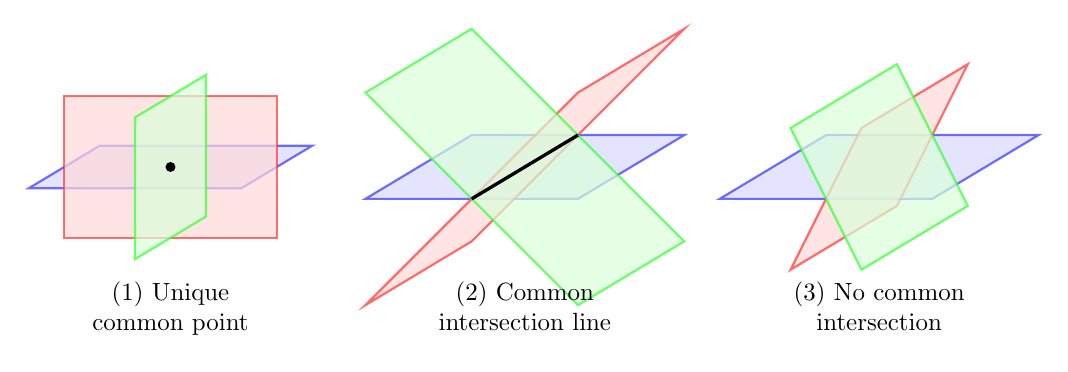
\begin{tikzpicture}[scale=0.9, every node/.style={scale=0.9}]
  % 1) Unique point
  \begin{scope}[shift={(0,0)}]
    \filldraw[fill=blue!15, draw=blue!80, thick, opacity=0.7] (1.00,-0.30) -- (2.00,0.30) -- (-1.00,0.30) -- (-2.00,-0.30) -- cycle;
    \filldraw[fill=red!15, draw=red!80, thick, opacity=0.7] (1.50,1.00) -- (-1.50,1.00) -- (-1.50,-1.00) -- (1.50,-1.00) -- cycle;
    \filldraw[fill=green!15, draw=green!80, thick, opacity=0.7] (-0.50,0.70) -- (0.50,1.30) -- (0.50,-0.70) -- (-0.50,-1.30) -- cycle;
    \fill[black] (0,0) circle (2pt);
    \node[align=center, below] at (0,-1.5) {(1) Unique\\common point};
  \end{scope}

  % 2) Common line
  \begin{scope}[shift={(5,0)}]
    \filldraw[fill=blue!15, draw=blue!80, thick, opacity=0.7] (0.75,-0.45) -- (2.25,0.45) -- (-0.75,0.45) -- (-2.25,-0.45) -- cycle;
    \filldraw[fill=red!15, draw=red!80, thick, opacity=0.7] (0.75,1.05) -- (2.25,1.95) -- (-0.75,-1.05) -- (-2.25,-1.95) -- cycle;
    \filldraw[fill=green!15, draw=green!80, thick, opacity=0.7] (0.75,-1.95) -- (2.25,-1.05) -- (-0.75,1.95) -- (-2.25,1.05) -- cycle;
    \draw[black, very thick] (0.75, 0.45) -- (-0.75, -0.45);
    \node[align=center, below] at (0,-1.5) {(2) Common\\intersection line};
  \end{scope}

  % 3) Prism (no common intersection)
  \begin{scope}[shift={(10,0)}]
    \filldraw[fill=blue!15, draw=blue!80, thick, opacity=0.7] (0.75,-0.45) -- (2.25,0.45) -- (-0.75,0.45) -- (-2.25,-0.45) -- cycle;
    \filldraw[fill=red!15, draw=red!80, thick, opacity=0.7] (-0.25,0.55) -- (1.25,1.45) -- (0.25,-0.55) -- (-1.25,-1.45) -- cycle;
    \filldraw[fill=green!15, draw=green!80, thick, opacity=0.7] (-1.25,0.55) -- (0.25,1.45) -- (1.25,-0.55) -- (-0.25,-1.45) -- cycle;
    \node[align=center, below] at (0,-1.5) {(3) No common\\intersection};
  \end{scope}
\end{tikzpicture}
\end{center}

\subsubsection*{Setting Up Systems}

To find a unique solution for $n$ unknown variables, you generally need $n$ independent linear equations. A common application is translating real-world scenarios into a $3 \times 3$ system of equations.

\bigskip

% ── Worked Example: Setting up a 3x3 system ──
\begin{problem}[Translating a Word Problem into a System]
A local bakery sells three types of cakes: chocolate, vanilla, and strawberry. The bakery records its sales and revenue for three consecutive days:
\begin{itemize}
  \item \textbf{Monday:} 2 chocolate, 3 vanilla, and 1 strawberry cake were sold for a total of \$115.
  \item \textbf{Tuesday:} 1 chocolate, 2 vanilla, and 2 strawberry cakes were sold for a total of \$110.
  \item \textbf{Wednesday:} 3 chocolate, 1 vanilla, and 3 strawberry cakes were sold for a total of \$165.
\end{itemize}

Assuming the price of each cake type remains constant, define appropriate variables and set up a system of three simultaneous linear equations that models this situation.
\end{problem}

\begin{solution}
\textbf{Step 1: Define the variables.} \\
Let $x$ = the price of a chocolate cake (in \$). \\
Let $y$ = the price of a vanilla cake (in \$). \\
Let $z$ = the price of a strawberry cake (in \$).

\medskip
\textbf{Step 2: Translate each day's sales into an equation.} \\
Monday's sales ($2$ choc, $3$ van, $1$ straw yield \$115):
\[ 2x + 3y + z = 115 \]
Tuesday's sales ($1$ choc, $2$ van, $2$ straw yield \$110):
\[ x + 2y + 2z = 110 \]
Wednesday's sales ($3$ choc, $1$ van, $3$ straw yield \$165):
\[ 3x + y + 3z = 165 \]

\medskip
\textbf{Step 3: State the final system.} \\
The system of simultaneous linear equations is:
\begin{align*}
2x + 3y + z &= 115 \\
x + 2y + 2z &= 110 \\
3x + y + 3z &= 165
\end{align*}

\emph{(Note: We will solve this exact system using matrices in the next topic!)}
\end{solution}

\begin{takeaways}
\item \textbf{Geometry of $3$ Variables:} Always visualize $3 \times 3$ systems as three flat planes in 3D space. When a unique solution exists, it is the common intersection point.
\item \textbf{Information Requirement:} Solving for 3 unknowns uniquely requires 3 independent pieces of information (equations). If you only have two equations, two independent consistent planes normally intersect in a line; parallel planes have no common points and coincident planes give a plane of solutions.
\item \textbf{Careful Translation:} When reading word problems, ensure the coefficients (quantities) align correctly with their corresponding variables (prices) in each equation.
\end{takeaways}

% Topic 7: Using Matrix Algebra for Systems of Linear Equations in More Than Two Variables
% Part of the Matrix Fundamentals section

\subsection{Using Matrix Algebra for Systems of Linear Equations in More Than Two Variables}

The elegance of matrix algebra is that the fundamental equation used to solve a system, $X = A^{-1}B$, remains exactly the same regardless of whether you are solving a $2 \times 2$ system, a $3 \times 3$ system, or a $100 \times 100$ system. 

The only difference is the computational effort required to find the inverse matrix, $A^{-1}$.

\bigskip

% ── Worked Example: Solving a 3x3 System using Matrices ──
\begin{problem}[Matrix Solution to a $3 \times 3$ System]
Recall the bakery word problem from the previous topic, which gave us the following system:
\begin{align*}
2x + 3y + z &= 115 \\
x + 2y + 2z &= 110 \\
3x + y + 3z &= 165
\end{align*}
Use matrix algebra to solve for $x, y$, and $z$, finding the exact price of each cake.
\end{problem}

\begin{solution}
\textbf{Step 1: Write the system in the form $AX = B$.} \\
\[
\begin{bmatrix} 2 & 3 & 1 \\ 1 & 2 & 2 \\ 3 & 1 & 3 \end{bmatrix} \begin{bmatrix} x \\ y \\ z \end{bmatrix} = \begin{bmatrix} 115 \\ 110 \\ 165 \end{bmatrix}
\]
Where $A$ is the $3 \times 3$ coefficient matrix, and $B$ is the constants matrix.

\medskip
\textbf{Step 2: Find the determinant of $A$.} \\
Expanding along the first row:
\begin{align*}
\det(A) &= 2 \begin{vmatrix} 2 & 2 \\ 1 & 3 \end{vmatrix} - 3 \begin{vmatrix} 1 & 2 \\ 3 & 3 \end{vmatrix} + 1 \begin{vmatrix} 1 & 2 \\ 3 & 1 \end{vmatrix} \\[6pt]
&= 2(6 - 2) - 3(3 - 6) + 1(1 - 6) \\
&= 2(4) - 3(-3) + 1(-5) \\
&= 8 + 9 - 5 = 12
\end{align*}
Since $\det(A) = 12 \neq 0$, a unique solution exists.

\medskip
\textbf{Step 3: Find the matrix of cofactors, $C$.} \\
Calculating the 9 cofactors (with the checkerboard sign pattern):
\begin{align*}
C_{11} &= +(6 - 2) = 4,   & C_{12} &= -(3 - 6) = 3,  & C_{13} &= +(1 - 6) = -5 \\
C_{21} &= -(9 - 1) = -8,  & C_{22} &= +(6 - 3) = 3,  & C_{23} &= -(2 - 9) = 7 \\
C_{31} &= +(6 - 2) = 4,   & C_{32} &= -(4 - 1) = -3, & C_{33} &= +(4 - 3) = 1
\end{align*}
So, the cofactor matrix is $C = \begin{bmatrix} 4 & 3 & -5 \\ -8 & 3 & 7 \\ 4 & -3 & 1 \end{bmatrix}$.

\medskip
\textbf{Step 4: Find the adjugate and inverse of $A$.} \\
Transpose $C$ to get the adjugate:
\[
\text{adj}(A) = C^T = \begin{bmatrix} 4 & -8 & 4 \\ 3 & 3 & -3 \\ -5 & 7 & 1 \end{bmatrix}
\]
The inverse is $A^{-1} = \frac{1}{\det(A)}\text{adj}(A) = \frac{1}{12} \begin{bmatrix} 4 & -8 & 4 \\ 3 & 3 & -3 \\ -5 & 7 & 1 \end{bmatrix}$.

\medskip
\textbf{Step 5: Solve for $X$ using $X = A^{-1}B$.}
\[
X = \frac{1}{12} \begin{bmatrix} 4 & -8 & 4 \\ 3 & 3 & -3 \\ -5 & 7 & 1 \end{bmatrix} \begin{bmatrix} 115 \\ 110 \\ 165 \end{bmatrix}
\]
Calculate the matrix product first:
\begin{align*}
X &= \frac{1}{12} \begin{bmatrix} 4(115) + (-8)(110) + 4(165) \\ 3(115) + 3(110) + (-3)(165) \\ -5(115) + 7(110) + 1(165) \end{bmatrix} \\[6pt]
X &= \frac{1}{12} \begin{bmatrix} 460 - 880 + 660 \\ 345 + 330 - 495 \\ -575 + 770 + 165 \end{bmatrix} = \frac{1}{12} \begin{bmatrix} 240 \\ 180 \\ 360 \end{bmatrix} = \begin{bmatrix} 20 \\ 15 \\ 30 \end{bmatrix}
\end{align*}

\medskip
\textbf{Conclusion:} \\
The variables are $x=20, y=15, z=30$. \\
The prices are \$20 for a chocolate cake, \$15 for a vanilla cake, and \$30 for a strawberry cake.
\end{solution}

\begin{takeaways}
\item \textbf{Universal Logic:} The framework $X = A^{-1}B$ scales to any number of dimensions. Only the mechanics of finding $A^{-1}$ change.
\item \textbf{Computational Load:} As systems get larger (e.g., $4 \times 4$), finding inverses by hand becomes highly prone to arithmetic errors. This is why computers and graphics cards are used to solve these systems in real life!
\item \textbf{Checking your work:} You can easily verify the final solution by substituting the values back into any of the original equations (e.g., $2(20) + 3(15) + 30 = 40 + 45 + 30 = 115$, which matches Monday's total).
\end{takeaways}

% Topic 8: Using Augmented Matrices for Systems of Equations
% Part of the Matrix Fundamentals section

\subsection{Using Augmented Matrices for Systems of Equations}

Finding the inverse of a $3 \times 3$ or larger matrix is computationally heavy. Furthermore, if a system has no solutions or infinitely many solutions, the inverse method fails because $\det(A) = 0$. 

A more robust and efficient method is \textbf{Gaussian elimination}, which uses \textbf{augmented matrices} and \textbf{elementary row operations}.

\subsubsection*{The Augmented Matrix}

Instead of writing three separate matrices ($A$, $X$, and $B$), we combine the coefficient matrix $A$ and the constant matrix $B$ into a single matrix, separated by a vertical line. For a $3 \times 3$ system, it looks like this:
\[
[A \,|\, B] = \left[ \begin{array}{ccc|c} 
a_{11} & a_{12} & a_{13} & b_1 \\ 
a_{21} & a_{22} & a_{23} & b_2 \\ 
a_{31} & a_{32} & a_{33} & b_3 
\end{array} \right]
\]

\subsubsection*{Elementary Row Operations}

Because each row represents an algebraic equation, we can perform operations on the rows without changing the solution to the system. There are three valid \textbf{elementary row operations}:
\begin{enumerate}
  \item \textbf{Swap:} Interchange any two rows (e.g., $R_1 \leftrightarrow R_2$).
  \item \textbf{Scale:} Multiply an entire row by a non-zero scalar (e.g., $R_2 \to \frac{1}{2}R_2$).
  \item \textbf{Add/Subtract:} Add a multiple of one row to another row (e.g., $R_3 \to R_3 - 2R_1$).
\end{enumerate}

\subsubsection*{Row Echelon Form (REF)}

The goal of Gaussian elimination is to use these operations to transform the augmented matrix into \textbf{Row Echelon Form}. In REF, the bottom-left corner of the matrix is filled with zeros, creating a "staircase" pattern:
\[
\left[ \begin{array}{ccc|c} 
1 & * & * & * \\ 
0 & 1 & * & * \\ 
0 & 0 & 1 & * 
\end{array} \right]
\]
Once in this form, the system can be easily solved from the bottom up using \textbf{back-substitution}.

\bigskip

% ── Worked Example: Gaussian Elimination ──
\begin{problem}[Gaussian Elimination]
Solve the following system of linear equations using an augmented matrix and row reduction:
\begin{align*}
x + y + z &= 6 \\
2x - y + 2z &= 6 \\
x + 2y - z &= 2
\end{align*}
\end{problem}

\begin{solution}
\textbf{Step 1: Write the augmented matrix.}
\[
\left[ \begin{array}{ccc|c} 
1 & 1 & 1 & 6 \\ 
2 & -1 & 2 & 6 \\ 
1 & 2 & -1 & 2 
\end{array} \right]
\]

\medskip
\textbf{Step 2: Eliminate the $x$-coefficients in Rows 2 and 3.} \\
To get a zero in $R_2$, column 1, we subtract $2 \times R_1$ from $R_2$ ($R_2 \to R_2 - 2R_1$):
\[
\left[ \begin{array}{ccc|c} 
1 & 1 & 1 & 6 \\ 
0 & -3 & 0 & -6 \\ 
1 & 2 & -1 & 2 
\end{array} \right]
\]
To get a zero in $R_3$, column 1, we subtract $R_1$ from $R_3$ ($R_3 \to R_3 - R_1$):
\[
\left[ \begin{array}{ccc|c} 
1 & 1 & 1 & 6 \\ 
0 & -3 & 0 & -6 \\ 
0 & 1 & -2 & -4 
\end{array} \right]
\]

\medskip
\textbf{Step 3: Simplify and eliminate the $y$-coefficient in Row 3.} \\
Let's simplify $R_2$ by dividing by $-3$ ($R_2 \to -\frac{1}{3}R_2$):
\[
\left[ \begin{array}{ccc|c} 
1 & 1 & 1 & 6 \\ 
0 & 1 & 0 & 2 \\ 
0 & 1 & -2 & -4 
\end{array} \right]
\]
Now, eliminate the $y$-coefficient in $R_3$ by subtracting $R_2$ ($R_3 \to R_3 - R_2$):
\[
\left[ \begin{array}{ccc|c} 
1 & 1 & 1 & 6 \\ 
0 & 1 & 0 & 2 \\ 
0 & 0 & -2 & -6 
\end{array} \right]
\]

\medskip
\textbf{Step 4: Finalize Row Echelon Form and Back-Substitute.} \\
Divide $R_3$ by $-2$ ($R_3 \to -\frac{1}{2}R_3$):
\[
\left[ \begin{array}{ccc|c} 
1 & 1 & 1 & 6 \\ 
0 & 1 & 0 & 2 \\ 
0 & 0 & 1 & 3 
\end{array} \right]
\]
Translate the matrix back into equations:
\begin{align*}
x + y + z &= 6 \quad \text{--- (1)} \\
y &= 2 \quad \text{--- (2)} \\
z &= 3 \quad \text{--- (3)}
\end{align*}
We already have $y=2$ and $z=3$. Substitute these back into equation (1):
\begin{align*}
x + (2) + (3) &= 6 \\
x + 5 &= 6 \\
x &= 1
\end{align*}

The unique solution is $x = 1, y = 2, z = 3$.
\end{solution}

\begin{takeaways}
\item \textbf{Computational Efficiency:} Gaussian elimination requires far fewer calculations than finding a $3 \times 3$ inverse, making it the preferred method for solving systems by hand.
\item \textbf{Detecting Anomalies:} If a system has no solution, row reduction will eventually produce an impossible row like $\left[ \begin{array}{ccc|c} 0 & 0 & 0 & 5 \end{array} \right]$, which algebraically means $0 = 5$. 
\item \textbf{Infinite Solutions:} If a system has infinite solutions, row reduction will produce a redundant row like $\left[ \begin{array}{ccc|c} 0 & 0 & 0 & 0 \end{array} \right]$, indicating one equation was just a multiple of another.
\end{takeaways}

% Topic 9: Matrices as Transformations
% Part of the Matrix Fundamentals section

\subsection{Matrices as Linear Transformations}

One of the most important applications of matrices is in representing geometric transformations. While you may be familiar with column vectors as representing points or translations, multiplying a vector by a matrix can scale, reflect, rotate, or shear that vector. 

A linear transformation can be thought of as a function that maps an input vector $\mathbf{v} = \begin{bmatrix} x \\ y \end{bmatrix}$ to an output vector $\mathbf{v'} = \begin{bmatrix} x' \\ y' \end{bmatrix}$ via matrix multiplication:
\[
\mathbf{v'} = A\mathbf{v} \quad \implies \quad \begin{bmatrix} x' \\ y' \end{bmatrix} = \begin{bmatrix} a & b \\ c & d \end{bmatrix} \begin{bmatrix} x \\ y \end{bmatrix}
\]

\subsubsection*{Common 2D Transformations}
Here are standard matrices for common geometric transformations in the 2D Cartesian plane:

\begin{center}
\renewcommand{\arraystretch}{1.5}
\begin{tabular}{p{2cm} p{4.5cm} p{6.5cm}}
\hline
\textbf{Transform} & \textbf{Matrix} & \textbf{Geometric Effect} \\
\hline
\textbf{Scaling} & 
$\begin{bmatrix} k_x & 0 \\ 0 & k_y \end{bmatrix}$ & 
Enlarges or shrinks shapes by factor $k_x$ in $x$-dir, $k_y$ in $y$-dir. \\

\textbf{Reflection} & 
$\begin{bmatrix} \cos 2\alpha & \sin 2\alpha \\ \sin 2\alpha & -\cos 2\alpha \end{bmatrix}$ & 
Reflects across a line through the origin making angle $\alpha$ with the positive $x$-axis ($y = x\tan\alpha$). \\

\textbf{Rotation} & 
$\begin{bmatrix} \cos\theta & -\sin\theta \\ \sin\theta & \cos\theta \end{bmatrix}$ & 
Rotates counter-clockwise by angle $\theta$ around the origin. \\

\textbf{Shear} & 
$\begin{bmatrix} 1 & k \\ 0 & 1 \end{bmatrix}$ (horizontal) \newline 
$\begin{bmatrix} 1 & 0 \\ k & 1 \end{bmatrix}$ (vertical) & 
Slants the shape along the axis by a factor $k$. \\
\hline
\end{tabular}
\end{center}

\subsubsection*{Composition of Transformations and Inverses}

If we apply a transformation $A$ and then a transformation $B$, this is equivalent to a single transformation given by the matrix product $BA$. Notice the order: $B(A\mathbf{v}) = (BA)\mathbf{v}$. 
Because matrix multiplication is generally \textbf{not commutative} ($AB \neq BA$), the order of transformations matters. For example, rotating an object and then reflecting it is usually different from reflecting it and then rotating it.

Furthermore, if a matrix $A$ represents a transformation, its inverse $A^{-1}$ (if it exists) represents \textbf{undoing} that transformation. The absolute value $|\det(A)|$ gives the area scale factor; the sign indicates orientation. If $\det(A) = 0$, the transformation collapses the 2D plane into a line or a point, making it non-invertible.

\begin{remark}[NSW HSC Heritage: Reflections and Rotations (1975--1980)]
A celebrated theorem examined in the NSW HSC 4~Unit examinations (notably 1975 Question~6 and 1976 Question~9) states that \textbf{the product of any two reflection matrices is a rotation matrix}.

Let $R_\alpha$ and $R_\beta$ be reflection matrices across lines inclined at angles $\alpha$ and $\beta$ respectively:
\[
R_\beta R_\alpha = \begin{bmatrix} \cos 2\beta & \sin 2\beta \\ \sin 2\beta & -\cos 2\beta \end{bmatrix} \begin{bmatrix} \cos 2\alpha & \sin 2\alpha \\ \sin 2\alpha & -\cos 2\alpha \end{bmatrix} = \begin{bmatrix} \cos 2(\beta - \alpha) & -\sin 2(\beta - \alpha) \\ \sin 2(\beta - \alpha) & \cos 2(\beta - \alpha) \end{bmatrix}.
\]
The composite transformation is a rotation through an angle $\theta = 2(\beta - \alpha)$, twice the angle between the two lines of reflection! Notice also that $\det(R_\alpha) = -\cos^2 2\alpha - \sin^2 2\alpha = -1$ (reversing orientation), while $\det(R_\beta R_\alpha) = (-1)(-1) = +1$ (preserving orientation), confirming geometrically why two reflections yield a rotation.
\end{remark}

\bigskip

\begin{problem}[Transformation Composition]
Let point $P$ have coordinates $(2, 3)$. 
\begin{enumerate}[label=\textbf{(\alph*)}]
    \item Find the coordinates of $P'$ after a counter-clockwise rotation of $90^\circ$ around the origin.
    \item Find the matrix that represents a reflection across the $x$-axis, followed by a counter-clockwise rotation of $90^\circ$.
    \item Use this combined matrix to transform point $P$.
\end{enumerate}
\end{problem}

\begin{solution}
\textbf{(a) Single Transformation} \\
The rotation matrix for $\theta = 90^\circ$ is $R_{90^\circ} = \begin{bmatrix} \cos 90^\circ & -\sin 90^\circ \\ \sin 90^\circ & \cos 90^\circ \end{bmatrix} = \begin{bmatrix} 0 & -1 \\ 1 & 0 \end{bmatrix}$.
Applying this to $P = \begin{bmatrix} 2 \\ 3 \end{bmatrix}$:
\[
P' = \begin{bmatrix} 0 & -1 \\ 1 & 0 \end{bmatrix} \begin{bmatrix} 2 \\ 3 \end{bmatrix} = \begin{bmatrix} -3 \\ 2 \end{bmatrix}
\]
So $P'$ is at $(-3, 2)$.

\medskip
\textbf{(b) Composition Matrix} \\
Let $M_1$ be the reflection across the $x$-axis: $M_1 = \begin{bmatrix} 1 & 0 \\ 0 & -1 \end{bmatrix}$. \\
Let $M_2$ be the $90^\circ$ rotation: $M_2 = \begin{bmatrix} 0 & -1 \\ 1 & 0 \end{bmatrix}$. \\
The combined transformation is $M = M_2 M_1$ (since $M_1$ acts first):
\[
M = \begin{bmatrix} 0 & -1 \\ 1 & 0 \end{bmatrix} \begin{bmatrix} 1 & 0 \\ 0 & -1 \end{bmatrix} = \begin{bmatrix} 0 & 1 \\ 1 & 0 \end{bmatrix}
\]
Notice that this resulting matrix corresponds to a reflection across the line $y = x$.

\medskip
\textbf{(c) Applying the Combined Matrix} \\
Applying $M$ to $P$:
\[
P'' = \begin{bmatrix} 0 & 1 \\ 1 & 0 \end{bmatrix} \begin{bmatrix} 2 \\ 3 \end{bmatrix} = \begin{bmatrix} 3 \\ 2 \end{bmatrix}
\]
So the final coordinate is $(3, 2)$.
\end{solution}

\begin{takeaways}
\item \textbf{Order Matters:} When chaining geometric transformations, you multiply the matrices from right to left.
\item \textbf{Geometric Meaning of Determinant:} If you apply the transformation matrix $M$ from part (b), $\det(M) = (0)(0) - (1)(1) = -1$. The absolute value of $1$ means the area is preserved, and the negative sign indicates that the orientation (e.g., clockwise vs counter-clockwise ordering of vertices) has been reversed, typical of a reflection.
\end{takeaways}

% Topic 10: Matrix Powers and Iteration
% Part of the Matrix Fundamentals section

\subsection{Matrix Powers, Iteration and Dynamical Systems}

We have seen how matrices can transform vectors. A surprising number of mathematical and real-world models rely on applying a transformation repeatedly to see how a system evolves over time. 

If we have an initial state represented by a vector $x_0$, applying a matrix transformation $A$ produces the next state:
\[
x_1 = Ax_0
\]
If we apply the same transformation again to get the subsequent state:
\[
x_2 = Ax_1 = A(Ax_0) = A^2 x_0
\]
This pattern continues. The state after $n$ steps is given by explicitly calculating the $n$-th power of the matrix $A$:
\[
x_n = A^n x_0
\]

This relationship $x_{n+1} = A x_n \implies x_n = A^n x_0$ is the foundational idea behind \textbf{dynamical systems}. It forms a conceptual bridge between basic matrix multiplication and advanced applications. 

\subsubsection*{Applications of Matrix Iteration}
By studying the long-term behaviour of $A^n$ as $n$ becomes very large ($n \to \infty$), we can answer questions about the stability and equilibrium of systems. For example:
\begin{itemize}[leftmargin=*]
  \item \textbf{Probability and Markov Chains:} Tracking the probabilities of states transitioning over time.
  \item \textbf{Graph Theory:} Finding the number of pathways of length $n$ between nodes in a network or computing total dominance scores (e.g., $A + A^2$).
  \item \textbf{Population Models:} Projecting future age demographics (like the Leslie matrix model).
  \item \textbf{Fibonacci and Recurrence Relations:} Expressing sequential terms compactly to compute the $n$-th term quickly.
\end{itemize}

\bigskip

\begin{problem}[Iterating a System]
Suppose the weather in a city is either Sunny (S) or Rainy (R) on a given day. The probability of tomorrow's weather depends only on today's weather, given by the transition rules:
\begin{itemize}
  \item If today is Sunny, tomorrow has a $80\%$ chance of being Sunny and $20\%$ chance of being Rainy.
  \item If today is Rainy, tomorrow has a $60\%$ chance of being Sunny and $40\%$ chance of being Rainy.
\end{itemize}

Let $x_n = \begin{bmatrix} P(\text{Sunny on day } n) \\ P(\text{Rainy on day } n) \end{bmatrix}$. 

\begin{enumerate}[label=\textbf{(\alph*)}]
    \item Construct the transition matrix $A$ such that $x_{n+1} = A x_n$.
    \item If Monday (day 0) is definitely Sunny, so $x_0 = \begin{bmatrix} 1 \\ 0 \end{bmatrix}$, find the probabilities for Wednesday (day 2) by calculating $x_2$.
    \item Calculate $A^2$ directly, and verify that $x_2 = A^2 x_0$.
\end{enumerate}
\end{problem}

\begin{solution}
\textbf{(a) Transition Matrix} \\
We place the probabilities of transitioning \emph{to} a state in the rows and \emph{from} a state in the columns:
\[
\text{To } S \quad \text{To } R \\
\]
\[
A = \begin{bmatrix} 0.8 & 0.6 \\ 0.2 & 0.4 \end{bmatrix} \begin{matrix} \text{From } S \\ \text{From } R \end{matrix}
\]
So $x_{n+1} = \begin{bmatrix} 0.8 & 0.6 \\ 0.2 & 0.4 \end{bmatrix} x_n$.

\medskip
\textbf{(b) Finding $x_2$ iteratively} \\
First, find $x_1$ (Tuesday):
\[
x_1 = A x_0 = \begin{bmatrix} 0.8 & 0.6 \\ 0.2 & 0.4 \end{bmatrix} \begin{bmatrix} 1 \\ 0 \end{bmatrix} = \begin{bmatrix} 0.8 \\ 0.2 \end{bmatrix}
\]
Next, find $x_2$ (Wednesday):
\[
x_2 = A x_1 = \begin{bmatrix} 0.8 & 0.6 \\ 0.2 & 0.4 \end{bmatrix} \begin{bmatrix} 0.8 \\ 0.2 \end{bmatrix} = \begin{bmatrix} 0.64 + 0.12 \\ 0.16 + 0.08 \end{bmatrix} = \begin{bmatrix} 0.76 \\ 0.24 \end{bmatrix}
\]
There is a $76\%$ chance of sun and $24\%$ chance of rain on Wednesday.

\medskip
\textbf{(c) Direct calculation via $A^2$} \\
\[
A^2 = \begin{bmatrix} 0.8 & 0.6 \\ 0.2 & 0.4 \end{bmatrix} \begin{bmatrix} 0.8 & 0.6 \\ 0.2 & 0.4 \end{bmatrix} = \begin{bmatrix} 0.64+0.12 & 0.48+0.24 \\ 0.16+0.08 & 0.12+0.16 \end{bmatrix} = \begin{bmatrix} 0.76 & 0.72 \\ 0.24 & 0.28 \end{bmatrix}
\]
Now calculate $A^2 x_0$:
\[
A^2 x_0 = \begin{bmatrix} 0.76 & 0.72 \\ 0.24 & 0.28 \end{bmatrix} \begin{bmatrix} 1 \\ 0 \end{bmatrix} = \begin{bmatrix} 0.76 \\ 0.24 \end{bmatrix}
\]
This perfectly matches our iterative result.
\end{solution}

\begin{takeaways}
\item \textbf{Efficiency:} For small $n$, iterating step-by-step ($x_1$, $x_2$) is easy. But for large $n$, calculating $A^n$ (often using computer software or advanced techniques like diagonalisation) and directly applying $x_n = A^n x_0$ is vastly more efficient.
\item \textbf{Long-Term Behaviour:} Repeatedly squaring a matrix (e.g., $A \to A^2 \to A^4 \to A^8$) is a quick way to see where a system eventually settles, known as the steady-state or equilibrium.
\end{takeaways}

% Topic 11: Dominance Matrices
% Part of the Matrix Fundamentals section

\subsection{Dominance Matrices}

Matrices are not only used for solving algebraic equations; they are incredibly powerful tools in discrete mathematics and network theory. A \textbf{dominance matrix} is used to represent and analyze directed relationships, such as the outcomes of a round-robin sports tournament or a ``pecking order'' in a group of animals.

\subsubsection*{Constructing the Dominance Matrix}

If a group of $n$ competitors play each other exactly once (no draws allowed), the results can be stored in an $n \times n$ matrix $D$:
\begin{itemize}[leftmargin=*]
  \item $d_{ij} = 1$ if competitor $i$ defeated competitor $j$.
  \item $d_{ij} = 0$ if competitor $i$ lost to competitor $j$.
\end{itemize}
The main diagonal is always entirely zeros, as a competitor cannot play themselves. 

\subsubsection*{Direct and Indirect Wins}

\begin{itemize}[leftmargin=*]
  \item \textbf{One-step dominance (Direct wins):} The sum of the elements in row $i$ of matrix $D$ gives the total number of matches won by competitor $i$. However, this often results in ties.
  \item \textbf{Two-step dominance (Indirect wins):} If Team A beats Team B, and Team B beats Team C, Team A has a two-step dominance over Team C. Mathematically, this is found by squaring the matrix to get $D^2$. This rewards teams for beating \emph{strong} opponents.
  \item \textbf{Total Dominance Score:} To break ties, we calculate a power score matrix $T = D + D^2$. The row sums of $T$ provide a much more robust ranking system.
\end{itemize}

\bigskip

% ── Worked Example: Ranking a Tournament ──
\begin{problem}[Tournament Rankings]
Four teams (A, B, C, and D) compete in a round-robin tournament. The results are as follows:
\begin{itemize}
  \item Team A defeated Teams B and C.
  \item Team B defeated Teams C and D.
  \item Team C defeated Team D.
  \item Team D defeated Team A.
\end{itemize}

\begin{enumerate}[label=\textbf{(\alph*)}]
  \item Construct the $4 \times 4$ dominance matrix $D$. Calculate the row sums to find the direct rankings and identify any ties.
  \item Calculate $D^2$, the two-step dominance matrix.
  \item Calculate the total dominance matrix $T = D + D^2$, and use its row sums to determine the final, tie-broken ranking of the four teams.
\end{enumerate}
\end{problem}

\begin{solution}
\textbf{(a) Matrix $D$ and Direct Rankings} \\
Following the rules, we place a $1$ in row $i$, column $j$ if the row team beat the column team.
\[
D = \begin{bmatrix} 
0 & 1 & 1 & 0 \\ 
0 & 0 & 1 & 1 \\ 
0 & 0 & 0 & 1 \\ 
1 & 0 & 0 & 0 
\end{bmatrix}
\]
Row Sums (Direct Wins):
\begin{itemize}
  \item Team A sum = 2
  \item Team B sum = 2
  \item Team C sum = 1
  \item Team D sum = 1
\end{itemize}
We have a tie for 1st place (A and B) and a tie for 3rd place (C and D).

\medskip
\textbf{(b) Matrix $D^2$ (Indirect Wins)} \\
Multiply $D$ by itself. For example, to find Row 1, Col 4 of $D^2$, we calculate $(0)(0) + (1)(1) + (1)(1) + (0)(0) = 2$. This means Team A has two indirect pathways to beat Team D (via B and via C).
\[
D^2 = D \times D = 
\begin{bmatrix} 0 & 1 & 1 & 0 \\ 0 & 0 & 1 & 1 \\ 0 & 0 & 0 & 1 \\ 1 & 0 & 0 & 0 \end{bmatrix}
\begin{bmatrix} 0 & 1 & 1 & 0 \\ 0 & 0 & 1 & 1 \\ 0 & 0 & 0 & 1 \\ 1 & 0 & 0 & 0 \end{bmatrix}
=
\begin{bmatrix} 
0 & 0 & 1 & 2 \\ 
1 & 0 & 0 & 1 \\ 
1 & 0 & 0 & 0 \\ 
0 & 1 & 1 & 0 
\end{bmatrix}
\]

\medskip
\textbf{(c) Total Dominance and Final Ranking} \\
Calculate $T = D + D^2$ by adding the corresponding elements:
\[
T = 
\begin{bmatrix} 0 & 1 & 1 & 0 \\ 0 & 0 & 1 & 1 \\ 0 & 0 & 0 & 1 \\ 1 & 0 & 0 & 0 \end{bmatrix}
+
\begin{bmatrix} 0 & 0 & 1 & 2 \\ 1 & 0 & 0 & 1 \\ 1 & 0 & 0 & 0 \\ 0 & 1 & 1 & 0 \end{bmatrix}
=
\begin{bmatrix} 
0 & 1 & 2 & 2 \\ 
1 & 0 & 1 & 2 \\ 
1 & 0 & 0 & 1 \\ 
1 & 1 & 1 & 0 
\end{bmatrix}
\]
Row Sums of $T$:
\begin{itemize}
  \item Team A = $0+1+2+2 = \textbf{5}$
  \item Team B = $1+0+1+2 = \textbf{4}$
  \item Team D = $1+1+1+0 = \textbf{3}$
  \item Team C = $1+0+0+1 = \textbf{2}$
\end{itemize}

\textbf{Final Ranking:} 1st: Team A, 2nd: Team B, 3rd: Team D, 4th: Team C. \\
The ties have been successfully broken!
\end{solution}

\begin{takeaways}
\item \textbf{Quality of Wins:} Team A and B both had 2 direct wins. However, Team A beat Team B (a strong team), giving A more indirect pathways to dominance. The $D+D^2$ method algebraically measures the "quality" of an opponent.
\item \textbf{Networks and Graphs:} Dominance matrices are adjacency matrices for directed graphs. Squaring the matrix algebraically counts the number of 2-step paths between nodes in a network.
\item \textbf{Real-World Algorithms:} This logic is the foundational mathematics behind modern search engines (like Google's PageRank algorithm), which rank web pages based on the quantity and quality of incoming links.
\end{takeaways}

% Topic 12: Leslie Matrices
% Part of the Matrix Fundamentals section

\subsection{Leslie Matrices}

Matrices can model dynamic, real-world systems that change over time. In biology and ecology, the \textbf{Leslie matrix} is a standard model used to predict the population growth of organisms by breaking the population down into distinct age groups (classes). Because females typically drive population reproduction rates, Leslie matrices generally only track the female portion of a population.

\subsubsection*{The Structure of a Leslie Matrix}

Suppose a population is divided into $n$ age classes of equal time duration. 
\begin{itemize}[leftmargin=*]
  \item Let $f_i$ be the \textbf{fecundity (fertility) rate}: the average number of female offspring born to a female in age class $i$.
  \item Let $s_i$ be the \textbf{survival rate}: the probability that a female in age class $i$ survives to enter age class $i+1$.
\end{itemize}

The Leslie matrix $L$ is a square $n \times n$ matrix built with a very specific layout:
\begin{itemize}[leftmargin=*]
  \item The \textbf{first row} contains the fecundity rates ($f_1, f_2, \dots, f_n$).
  \item The \textbf{sub-diagonal} (the diagonal immediately below the main diagonal) contains the survival rates ($s_1, s_2, \dots, s_{n-1}$).
  \item All other entries are exactly zero.
\end{itemize}

For a 3-age-class population, the matrix looks like this:
\[
L = \begin{bmatrix} 
f_1 & f_2 & f_3 \\ 
s_1 & 0 & 0 \\ 
0 & s_2 & 0 
\end{bmatrix}
\]

\subsubsection*{Population Projection}

If we represent the number of individuals in each age class at time $t$ as a column matrix (a state vector) $\mathbf{n}_t$, we can find the population at the next time interval by multiplying by $L$:
\[
\mathbf{n}_{t+1} = L \mathbf{n}_t
\]
To project $k$ time periods into the future from an initial population $\mathbf{n}_0$, we use matrix exponentiation:
\[
\mathbf{n}_{k} = L^k \mathbf{n}_0
\]

\bigskip

% ── Worked Example: Population Projection ──
\begin{problem}[Projecting a Rodent Population]
A species of rodent is divided into three age classes, each spanning one month: 0--1 month, 1--2 months, and 2--3 months. The maximum lifespan is 3 months.
\begin{itemize}
  \item \textbf{Fertility rates:} Class 1 females produce $0$ offspring. Class 2 females produce $2.0$ offspring. Class 3 females produce $1.5$ offspring.
  \item \textbf{Survival rates:} $40\%$ ($0.4$) of Class 1 survive to Class 2. $30\%$ ($0.3$) of Class 2 survive to Class 3.
  \item \textbf{Initial Population ($\mathbf{n}_0$):} There are currently 100 females in Class 1, 50 in Class 2, and 20 in Class 3.
\end{itemize}

\begin{enumerate}[label=\textbf{(\alph*)}]
  \item Construct the Leslie matrix, $L$, for this population.
  \item Calculate the population state vector after 1 month ($\mathbf{n}_1$).
  \item Calculate the population state vector after 2 months ($\mathbf{n}_2$).
\end{enumerate}
\end{problem}

\begin{solution}
\textbf{(a) Construct the Leslie matrix} \\
Row 1 contains the fertility rates: $0, 2.0, 1.5$. \\
The sub-diagonal contains the survival rates: $0.4$ and $0.3$.
\[
L = \begin{bmatrix} 
0 & 2.0 & 1.5 \\ 
0.4 & 0 & 0 \\ 
0 & 0.3 & 0 
\end{bmatrix}
\]

\medskip
\textbf{(b) Population after 1 month ($\mathbf{n}_1$)} \\
Multiply the Leslie matrix by the initial population vector $\mathbf{n}_0$:
\[
\mathbf{n}_1 = L \mathbf{n}_0 = 
\begin{bmatrix} 0 & 2.0 & 1.5 \\ 0.4 & 0 & 0 \\ 0 & 0.3 & 0 \end{bmatrix}
\begin{bmatrix} 100 \\ 50 \\ 20 \end{bmatrix}
= 
\begin{bmatrix} 
0(100) + 2.0(50) + 1.5(20) \\ 
0.4(100) + 0(50) + 0(20) \\ 
0(100) + 0.3(50) + 0(20) 
\end{bmatrix}
\]
\[
\mathbf{n}_1 = \begin{bmatrix} 0 + 100 + 30 \\ 40 \\ 15 \end{bmatrix} = \begin{bmatrix} 130 \\ 40 \\ 15 \end{bmatrix}
\]
After 1 month, there are 130 newborns, 40 adults (1-2 mo), and 15 elders (2-3 mo).

\medskip
\textbf{(c) Population after 2 months ($\mathbf{n}_2$)} \\
Multiply the Leslie matrix by the new population vector $\mathbf{n}_1$:
\[
\mathbf{n}_2 = L \mathbf{n}_1 = 
\begin{bmatrix} 0 & 2.0 & 1.5 \\ 0.4 & 0 & 0 \\ 0 & 0.3 & 0 \end{bmatrix}
\begin{bmatrix} 130 \\ 40 \\ 15 \end{bmatrix}
= 
\begin{bmatrix} 
0(130) + 2.0(40) + 1.5(15) \\ 
0.4(130) + 0(40) + 0(15) \\ 
0(130) + 0.3(40) + 0(15) 
\end{bmatrix}
\]
\[
\mathbf{n}_2 = \begin{bmatrix} 0 + 80 + 22.5 \\ 52 \\ 12 \end{bmatrix} = \begin{bmatrix} 102.5 \\ 52 \\ 12 \end{bmatrix}
\]
\emph{(Note: In mathematical biology, it is standard practice to keep decimals during intermediate calculation steps to avoid compounding rounding errors, and only round to whole animals when stating the final interpretive answer. So we have roughly 103 newborns, 52 adults, and 12 elders).}
\end{solution}

\begin{takeaways}
\item \textbf{Structured Flow:} The rigid structure of the Leslie matrix ensures mathematical logic: the top row calculates all new births and drops them into age class 1, while the sub-diagonal pushes the survivors from class $i$ down into class $i+1$.
\item \textbf{Iteration:} A system that updates based on its previous state ($\mathbf{n}_{t+1} = L \mathbf{n}_t$) is called a dynamical system. Matrices are perfect for iterating large blocks of data simultaneously.
\item \textbf{Long-term Behavior:} While outside the scope of this topic, the long-term survival or extinction of a population depends entirely on the largest \emph{eigenvalue} of its Leslie matrix!
\end{takeaways}


\section{Part 1: Worked Problems}

\subsection{Basic}
\begin{problem}[School Demographics Matrix]
Based on the demographic data provided in the school census:
At a certain school, there are $110$ girls and $110$ boys in Year 7. The numbers of girls and boys in the other year levels are $120$ and $105$ in Year 8, $140$ and $130$ in Year 9, $100$ and $95$ in Year 10, $90$ and $85$ in Year 11, and $60$ and $65$ in Year 12.

\begin{enumerate}[label=\textbf{(\alph*)}]
  \item Summarise this information in a $6 \times 2$ matrix, $S$, where the rows represent the year levels (7 to 12) and the columns represent the gender (girls, boys).
  \item Define a column matrix $C$ such that the matrix product $SC$ results in a $6 \times 1$ matrix representing the total number of students in each year level. Calculate $SC$.
  \item Define a row matrix $R$ such that the matrix product $RS$ results in a $1 \times 2$ matrix representing the total number of girls and boys in the school overall. Calculate $RS$.
  \item The school receives an extracurricular grant of $\$50$ per girl and $\$45$ per boy. Write down a column matrix $G$ representing these amounts, and calculate the product $SG$ to find the total grant amount allocated to each year level.
\end{enumerate}
\end{problem}

\begin{hint}
\begin{itemize}
  \item \textbf{Part (a):} Organise the data sequentially. Ensure your rows correspond to Years 7 through 12, and the first and second columns correspond to girls and boys, respectively.
  \item \textbf{Part (b):} To sum the elements across the rows of a matrix using matrix multiplication, you need to post-multiply by a column matrix of $1$s. Check your dimensions: a $(6 \times 2)$ matrix multiplied by a $(2 \times 1)$ matrix yields a $(6 \times 1)$ matrix.
  \item \textbf{Part (c):} To sum the elements down the columns, you must pre-multiply by a row matrix of $1$s. Verify the dimensions: $(1 \times 6)$ multiplied by $(6 \times 2)$.
  \item \textbf{Part (d):} Matrix multiplication pairs the row elements of the first matrix with the column elements of the second matrix. Make sure the $\$50$ aligns with the girls' column and the $\$45$ aligns with the boys' column.
\end{itemize}
\end{hint}

\begin{solution}
\textbf{(a)} \\
$S = \begin{bmatrix} 110 & 110 \\ 120 & 105 \\ 140 & 130 \\ 100 & 95 \\ 90 & 85 \\ 60 & 65 \end{bmatrix}$

\medskip
\textbf{(b)} \\
$C = \begin{bmatrix} 1 \\ 1 \end{bmatrix}$, \quad
$SC = \begin{bmatrix} 110 & 110 \\ 120 & 105 \\ 140 & 130 \\ 100 & 95 \\ 90 & 85 \\ 60 & 65 \end{bmatrix} \begin{bmatrix} 1 \\ 1 \end{bmatrix} = \begin{bmatrix} 220 \\ 225 \\ 270 \\ 195 \\ 175 \\ 125 \end{bmatrix}$

\medskip
\textbf{(c)} \\
$R = \begin{bmatrix} 1 & 1 & 1 & 1 & 1 & 1 \end{bmatrix}$ \\
$RS = \begin{bmatrix} 1 & 1 & 1 & 1 & 1 & 1 \end{bmatrix} \begin{bmatrix} 110 & 110 \\ 120 & 105 \\ 140 & 130 \\ 100 & 95 \\ 90 & 85 \\ 60 & 65 \end{bmatrix} = \begin{bmatrix} 620 & 590 \end{bmatrix}$

\medskip
\textbf{(d)} \\
$G = \begin{bmatrix} 50 \\ 45 \end{bmatrix}$, \quad
$SG = \begin{bmatrix} 110 & 110 \\ 120 & 105 \\ 140 & 130 \\ 100 & 95 \\ 90 & 85 \\ 60 & 65 \end{bmatrix} \begin{bmatrix} 50 \\ 45 \end{bmatrix} = \begin{bmatrix} 10450 \\ 10725 \\ 12850 \\ 9275 \\ 8325 \\ 5925 \end{bmatrix}$
\end{solution}

\begin{takeaways}
\item \textbf{Data Organisation:} Matrices are powerful tools for neatly organising and storing real-world demographic data.
\item \textbf{Summation Vectors:} Matrix multiplication using vectors of $1$s is an efficient algebraic method for summing rows or columns of a data matrix without writing out lengthy addition equations.
\item \textbf{Dimensionality Checks:} Always verify conformability before multiplying matrices. The number of columns in the leading matrix must equal the number of rows in the trailing matrix (e.g., $m \times n$ multiplied by $n \times p$ gives an $m \times p$ matrix).
\end{takeaways}


\subsection{Medium}
\begin{problem}[Matrix Properties and Transformations]
Consider a general $2 \times 2$ matrix $A = \begin{bmatrix} p & q \\ r & s \end{bmatrix}$ and its associated adjugate matrix $A^* = \begin{bmatrix} s & -q \\ -r & p \end{bmatrix}$.

\begin{enumerate}[label=\textbf{(\alph*)}]
    \item Evaluate the matrix product $A A^*$ and express the result in the form $kI$, where $I$ is the $2 \times 2$ identity matrix and $k$ is a scalar expressed in terms of $p, q, r,$ and $s$.
    \item Given that $k \neq 0$, use your result from part (a) to algebraically deduce the standard expression for the inverse matrix, $A^{-1}$.
    \item Evaluate the reverse product $A^* A$ and hence show that for this specific pair of matrices, multiplication is commutative.
    \item A linear transformation in the plane is represented by the matrix $M = \begin{bmatrix} 2x & 3 \\ 8 & x \end{bmatrix}$. Using the concept of $k$ from part (a), determine the exact possible values of $x$ for which this transformation cannot be reversed (i.e., the matrix is singular).
\end{enumerate}
\end{problem}

\begin{hint}
\begin{itemize}
    \item \textbf{Part (a):} Perform standard row-by-column matrix multiplication. Expand the terms, simplify the diagonals, and factor out any common algebraic expressions to reveal the identity matrix.
    \item \textbf{Part (b):} Recall that the definition of an inverse matrix is $A A^{-1} = I$. Take your equation from part (a), $A A^* = kI$, and manipulate it algebraically to isolate $I$ on one side of the equation.
    \item \textbf{Part (c):} Multiply the matrices again, but this time with $A^*$ on the left and $A$ on the right. Compare the resulting matrix to the one you found in part (a).
    \item \textbf{Part (d):} A matrix transformation does not have an inverse when its associated scalar $k$ (the determinant) is equal to zero. Set up an equation for $k = 0$ using the elements of matrix $M$ and solve for $x$.
\end{itemize}
\end{hint}

\begin{solution}
\textbf{(a)} \\
$A A^* = \begin{bmatrix} p & q \\ r & s \end{bmatrix} \begin{bmatrix} s & -q \\ -r & p \end{bmatrix} = \begin{bmatrix} ps-qr & -pq+qp \\ rs-sr & -rq+sp \end{bmatrix} = \begin{bmatrix} ps-qr & 0 \\ 0 & ps-qr \end{bmatrix}$ \\
Factoring out the common term: $A A^* = (ps-qr)\begin{bmatrix} 1 & 0 \\ 0 & 1 \end{bmatrix} = (ps-qr)I$. \\
Therefore, $k = ps - qr$.

\medskip
\textbf{(b)} \\
From part (a), we have $A A^* = (ps-qr)I$. \\
Assuming $ps-qr \neq 0$, we can divide both sides by this scalar: \\
$A \left( \frac{1}{ps-qr} A^* \right) = I$ \\
Since $A A^{-1} = I$, it follows that $A^{-1} = \frac{1}{ps-qr} \begin{bmatrix} s & -q \\ -r & p \end{bmatrix}$.

\medskip
\textbf{(c)} \\
$A^* A = \begin{bmatrix} s & -q \\ -r & p \end{bmatrix} \begin{bmatrix} p & q \\ r & s \end{bmatrix} = \begin{bmatrix} sp-qr & sq-qs \\ -rp+pr & -rq+ps \end{bmatrix} = \begin{bmatrix} ps-qr & 0 \\ 0 & ps-qr \end{bmatrix} = (ps-qr)I$ \\
Since $A A^* = (ps-qr)I$ and $A^* A = (ps-qr)I$, we have shown that $A A^* = A^* A$. Thus, multiplication of a matrix by its adjugate is commutative.

\medskip
\textbf{(d)} \\
For the transformation to have no inverse, $k = ps - qr = 0$. \\
For matrix $M$, $p = 2x$, $q = 3$, $r = 8$, and $s = x$. \\
$k = (2x)(x) - (3)(8) = 2x^2 - 24$ \\
Setting $k = 0$: $2x^2 - 24 = 0 \implies x^2 = 12 \implies x = \pm\sqrt{12} = \pm2\sqrt{3}$.
\end{solution}

\begin{takeaways}
\item \textbf{Determinant:} The scalar value $k = ps - qr$ derived in part (a) is the determinant of a $2 \times 2$ matrix. It is the fundamental factor that dictates whether a matrix has an inverse.
\item \textbf{Commutativity of Inverses:} While general matrix multiplication is strictly non-commutative ($AB \neq BA$), a matrix and its adjugate (or inverse) are a special exception where multiplication order does not change the result.
\item \textbf{Singular Matrices:} Matrices with a determinant of zero are called singular. Geometrically, these matrices represent transformations that collapse 2D space into a 1D line or a point, which is why the mapping cannot be algebraically reversed.
\end{takeaways}


\begin{problem}[Matrix Algebra and Commutativity]
Consider general $2 \times 2$ matrices $A$ and $B$.

\begin{enumerate}[label=\textbf{(\alph*)}]
    \item By expanding the product, show that $(A+B)^2 = A^2 + AB + BA + B^2$.
    \item Hence, state the necessary mathematical condition for matrices $A$ and $B$ such that the standard binomial expansion $(A+B)^2 = A^2 + 2AB + B^2$ is valid.
    \item Let $A = \begin{bmatrix} 1 & 0 \\ 0 & -1 \end{bmatrix}$ representing a reflection in the x-axis, and $B = \begin{bmatrix} k & 0 \\ 0 & k \end{bmatrix}$ representing a dilation by scale factor $k$. Verify algebraically that for these specific matrices, $(A+B)^2 = A^2 + 2AB + B^2$.
    \item Let $C = \begin{bmatrix} 0 & 1 \\ 1 & 0 \end{bmatrix}$ and $D = \begin{bmatrix} 0 & -1 \\ 1 & 0 \end{bmatrix}$. Evaluate $(C+D)^2$ and $C^2 + 2CD + D^2$, demonstrating they are not equal, and explain why this algebraic difference occurs in terms of matrix multiplication properties.
\end{enumerate}
\end{problem}

\begin{hint}
\begin{itemize}
    \item \textbf{Part (a):} Write $(A+B)^2$ as $(A+B)(A+B)$ and apply the distributive law carefully, ensuring you maintain the exact left-to-right order of matrix multiplication.
    \item \textbf{Part (b):} Compare your expanded result from part (a) to the target expression $A^2 + 2AB + B^2$. What must the middle terms $AB + BA$ simplify to?
    \item \textbf{Part (c):} Calculate the individual products $AB$ and $BA$ first. Check if they satisfy the condition you identified in part (b).
    \item \textbf{Part (d):} For the first expression, perform the matrix addition $C+D$ before squaring the result. For the second expression, calculate $C^2$, $D^2$, and $CD$ separately before summing them.
\end{itemize}
\end{hint}

\begin{solution}
\textbf{(a)} \\
$(A+B)^2 = (A+B)(A+B) = A(A+B) + B(A+B) = A^2 + AB + BA + B^2$.

\medskip
\textbf{(b)} \\
For $A^2 + AB + BA + B^2$ to equal $A^2 + 2AB + B^2$, we must have: \\
$AB + BA = 2AB \implies BA = AB$. \\
The necessary condition is that matrices $A$ and $B$ must commute.

\medskip
\textbf{(c)} \\
$AB = \begin{bmatrix} 1 & 0 \\ 0 & -1 \end{bmatrix} \begin{bmatrix} k & 0 \\ 0 & k \end{bmatrix} = \begin{bmatrix} k & 0 \\ 0 & -k \end{bmatrix}$ \\
$BA = \begin{bmatrix} k & 0 \\ 0 & k \end{bmatrix} \begin{bmatrix} 1 & 0 \\ 0 & -1 \end{bmatrix} = \begin{bmatrix} k & 0 \\ 0 & -k \end{bmatrix}$ \\
Since $AB = BA$, the matrices commute, and therefore the binomial expansion $(A+B)^2 = A^2 + 2AB + B^2$ holds valid for this specific pair.

\medskip
\textbf{(d)} \\
$C+D = \begin{bmatrix} 0 & 1 \\ 1 & 0 \end{bmatrix} + \begin{bmatrix} 0 & -1 \\ 1 & 0 \end{bmatrix} = \begin{bmatrix} 0 & 0 \\ 2 & 0 \end{bmatrix}$. \\
$(C+D)^2 = \begin{bmatrix} 0 & 0 \\ 2 & 0 \end{bmatrix} \begin{bmatrix} 0 & 0 \\ 2 & 0 \end{bmatrix} = \begin{bmatrix} 0 & 0 \\ 0 & 0 \end{bmatrix}$. \\
Next, evaluating the components of the expanded form: \\
$C^2 = \begin{bmatrix} 1 & 0 \\ 0 & 1 \end{bmatrix} = I$ and $D^2 = \begin{bmatrix} -1 & 0 \\ 0 & -1 \end{bmatrix} = -I$. \\
$CD = \begin{bmatrix} 0 & 1 \\ 1 & 0 \end{bmatrix} \begin{bmatrix} 0 & -1 \\ 1 & 0 \end{bmatrix} = \begin{bmatrix} 1 & 0 \\ 0 & -1 \end{bmatrix}$. \\
$C^2 + 2CD + D^2 = I + 2\begin{bmatrix} 1 & 0 \\ 0 & -1 \end{bmatrix} - I = \begin{bmatrix} 2 & 0 \\ 0 & -2 \end{bmatrix}$. \\
Since $\begin{bmatrix} 0 & 0 \\ 0 & 0 \end{bmatrix} \neq \begin{bmatrix} 2 & 0 \\ 0 & -2 \end{bmatrix}$, the expressions are unequal. This occurs because general matrix multiplication is non-commutative ($CD \neq DC$), preventing the cross-terms from simplifying to $2CD$.
\end{solution}

\begin{takeaways}
\item \textbf{Matrix Non-Commutativity:} The most critical difference between standard real number algebra and matrix algebra is that matrix multiplication is generally non-commutative ($AB \neq BA$).
\item \textbf{Binomial Expansion:} Standard polynomial identities like $(x+y)^2 = x^2+2xy+y^2$ cannot be blindly applied to matrices unless the specific matrices are proven to commute.
\item \textbf{Geometric Connection:} The algebraic failure of commutativity mirrors the geometric reality of transformations. For instance, applying a reflection then a rotation often results in a different final orientation compared to applying the rotation then the reflection.
\end{takeaways}


\subsection{Advanced}
\begin{problem}[Matrix Inverses and Matrix Equations]
Let $A$ and $B$ be $2 \times 2$ matrices defined as $A = \begin{bmatrix} k & 2 \\ -1 & 1 \end{bmatrix}$ and $B = \begin{bmatrix} 1 & -1 \\ 2 & 3 \end{bmatrix}$, where $k$ is a real constant.

\begin{enumerate}[label=\textbf{(\alph*)}]
    \item Determine the determinant of $A$ in terms of $k$, and hence state the value of $k$ for which matrix $A$ is singular.
    \item Let $k = 3$. Determine the inverse matrices $A^{-1}$ and $B^{-1}$.
    \item For $k = 3$, calculate the matrix product $AB$ and hence determine $(AB)^{-1}$.
    \item Evaluate the product $B^{-1}A^{-1}$ to verify the property $(AB)^{-1} = B^{-1}A^{-1}$. Hence, use this property to make the matrix $X$ the subject of the matrix equation $ABX = C$, where $C$ is a $2 \times 2$ matrix.
\end{enumerate}
\end{problem}

\begin{hint}
\begin{itemize}
    \item \textbf{Part (a):} The determinant of a $2 \times 2$ matrix $\begin{bmatrix} a & b \\ c & d \end{bmatrix}$ is $ad - bc$. A matrix is singular (has no inverse) when its determinant equals zero.
    \item \textbf{Part (b):} Use the formula for the inverse of a $2 \times 2$ matrix: $\frac{1}{\det(M)} \begin{bmatrix} d & -b \\ -c & a \end{bmatrix}$.
    \item \textbf{Part (c):} Multiply matrix $A$ by matrix $B$ using the standard row-by-column method. Then find the inverse of the resulting $2 \times 2$ matrix.
    \item \textbf{Part (d):} Multiply $B^{-1}$ (on the left) by $A^{-1}$ (on the right) and factor out the scalar multipliers. To solve $ABX = C$, remember that you must multiply both sides of the equation by the inverse of $AB$ on the left.
\end{itemize}
\end{hint}

\begin{solution}
\textbf{(a)} \\
$\det(A) = (k)(1) - (2)(-1) = k + 2$. \\
For matrix $A$ to be singular, $\det(A) = 0$. Therefore, $k = -2$.

\medskip
\textbf{(b)} \\
Given $k = 3$, $A = \begin{bmatrix} 3 & 2 \\ -1 & 1 \end{bmatrix}$. \\
$\det(A) = 3 + 2 = 5$. Thus, $A^{-1} = \frac{1}{5}\begin{bmatrix} 1 & -2 \\ 1 & 3 \end{bmatrix}$. \\
$\det(B) = (1)(3) - (-1)(2) = 3 + 2 = 5$. Thus, $B^{-1} = \frac{1}{5}\begin{bmatrix} 3 & 1 \\ -2 & 1 \end{bmatrix}$.

\medskip
\textbf{(c)} \\
$AB = \begin{bmatrix} 3 & 2 \\ -1 & 1 \end{bmatrix} \begin{bmatrix} 1 & -1 \\ 2 & 3 \end{bmatrix} = \begin{bmatrix} 3(1)+2(2) & 3(-1)+2(3) \\ -1(1)+1(2) & -1(-1)+1(3) \end{bmatrix} = \begin{bmatrix} 7 & 3 \\ 1 & 4 \end{bmatrix}$. \\
$\det(AB) = (7)(4) - (3)(1) = 28 - 3 = 25$. \\
$(AB)^{-1} = \frac{1}{25}\begin{bmatrix} 4 & -3 \\ -1 & 7 \end{bmatrix}$.

\medskip
\textbf{(d)} \\
$B^{-1}A^{-1} = \left( \frac{1}{5}\begin{bmatrix} 3 & 1 \\ -2 & 1 \end{bmatrix} \right) \left( \frac{1}{5}\begin{bmatrix} 1 & -2 \\ 1 & 3 \end{bmatrix} \right) = \frac{1}{25} \begin{bmatrix} 3(1)+1(1) & 3(-2)+1(3) \\ -2(1)+1(1) & -2(-2)+1(3) \end{bmatrix} = \frac{1}{25}\begin{bmatrix} 4 & -3 \\ -1 & 7 \end{bmatrix}$. \\
This verifies that $(AB)^{-1} = B^{-1}A^{-1}$. \\
To solve $ABX = C$: \\
$(AB)^{-1}(AB)X = (AB)^{-1}C$ \\
$IX = (AB)^{-1}C$ \\
$X = B^{-1}A^{-1}C$.
\end{solution}

\begin{takeaways}
\item \textbf{The "Socks and Shoes" Property:} The inverse of a matrix product reverses the order of the original matrices: $(AB)^{-1} = B^{-1}A^{-1}$.
\item \textbf{Matrix Algebra in Equations:} When isolating a matrix variable (like $X$ in $ABX=C$), you must respect the non-commutative nature of matrices by multiplying by the inverse on the correct side (in this case, pre-multiplying on the left).
\item \textbf{Determinant of a Product:} Notice that $\det(AB) = 25$, while $\det(A) = 5$ and $\det(B) = 5$. This verifies another key property: $\det(AB) = \det(A) \times \det(B)$.
\end{takeaways}


\begin{problem}[Matrix Inverses and the Zero Matrix]
Let $A, B, C,$ and $D$ be $2 \times 2$ matrices, where $O$ is the zero matrix and $I$ is the identity matrix.

\begin{enumerate}[label=\textbf{(\alph*)}]
    \item Assume $A$ is an invertible matrix and that $AB = O$. Prove algebraically that $B$ must be the zero matrix.
    \item Suppose instead that $C$ and $D$ are both strictly non-zero matrices, yet their product is the zero matrix ($CD = O$). By referencing your proof in part (a), deduce whether $C$ can be an invertible matrix. Support your answer with logical reasoning.
    \item A matrix $M$ is defined as being self-inverse if $M^{-1} = M$. By showing this implies $M^2 = I$, determine the algebraic condition on real numbers $a, b,$ and $c$ such that $M = \begin{bmatrix} a & b \\ c & -a \end{bmatrix}$ is a self-inverse matrix.
    \item Using your condition from part (c), construct a specific matrix $M$ where $a = 3$, and $b$ and $c$ are integers. Verify that your chosen matrix is self-inverse by explicitly evaluating $M^2$.
\end{enumerate}
\end{problem}

\begin{hint}
\begin{itemize}
    \item \textbf{Part (a):} Start with the given equation $AB = O$. Since $A$ is invertible, you are permitted to pre-multiply both sides of the equation by $A^{-1}$. What does $A^{-1}A$ simplify to?
    \item \textbf{Part (b):} Use a proof by contradiction. What would happen if $C$ \textit{was} invertible? Apply the exact same logic established in part (a) and compare the result to the condition that $D$ is a non-zero matrix.
    \item \textbf{Part (c):} Multiply both sides of $M^{-1} = M$ by $M$. Then, square the given matrix $M = \begin{bmatrix} a & b \\ c & -a \end{bmatrix}$ using standard row-by-column multiplication and equate the resulting elements to the corresponding elements of the identity matrix, $I$.
    \item \textbf{Part (d):} Substitute $a=3$ into your condition from part (c). Find two integers $b$ and $c$ that multiply together to satisfy the equation, construct the matrix, and manually multiply $M \times M$ to check it yields $I$.
\end{itemize}
\end{hint}

\begin{solution}
\textbf{(a)} \\
Given $AB = O$ and $A$ is invertible, $A^{-1}$ exists. Pre-multiplying both sides by $A^{-1}$: \\
$A^{-1}(AB) = A^{-1}O$ \\
$(A^{-1}A)B = O$ \\
$IB = O \implies B = O$.

\medskip
\textbf{(b)} \\
Assume for the sake of contradiction that $C$ is invertible. \\
Then, given $CD = O$, we could pre-multiply by $C^{-1}$ to get $C^{-1}(CD) = C^{-1}O \implies D = O$. \\
However, the problem states that $D$ is a non-zero matrix. This is a contradiction. Therefore, the assumption that $C$ is invertible must be false; $C$ must be a singular matrix.

\medskip
\textbf{(c)} \\
If $M^{-1} = M$, then multiplying both sides by $M$ gives $MM^{-1} = MM \implies I = M^2$. \\
Evaluating $M^2$: \\
$M^2 = \begin{bmatrix} a & b \\ c & -a \end{bmatrix} \begin{bmatrix} a & b \\ c & -a \end{bmatrix} = \begin{bmatrix} a^2+bc & ab-ab \\ ac-ac & bc+(-a)^2 \end{bmatrix} = \begin{bmatrix} a^2+bc & 0 \\ 0 & a^2+bc \end{bmatrix}$. \\
For $M^2 = I = \begin{bmatrix} 1 & 0 \\ 0 & 1 \end{bmatrix}$, we must have the condition: $a^2 + bc = 1$.

\medskip
\textbf{(d)} \\
Let $a=3$. From part (c), $3^2 + bc = 1 \implies 9 + bc = 1 \implies bc = -8$. \\
Choose integers $b = 2$ and $c = -4$ (other integer pairs like $4, -2$ are also valid). \\
$M = \begin{bmatrix} 3 & 2 \\ -4 & -3 \end{bmatrix}$. \\
Verification: \\
$M^2 = \begin{bmatrix} 3 & 2 \\ -4 & -3 \end{bmatrix} \begin{bmatrix} 3 & 2 \\ -4 & -3 \end{bmatrix} = \begin{bmatrix} 9-8 & 6-6 \\ -12+12 & -8+9 \end{bmatrix} = \begin{bmatrix} 1 & 0 \\ 0 & 1 \end{bmatrix} = I$.
\end{solution}

\begin{takeaways}
\item \textbf{Zero Product Property Failure:} In real number algebra, $xy=0$ implies $x=0$ or $y=0$. In matrix algebra, $CD=O$ does \textit{not} necessarily mean $C=O$ or $D=O$. Non-zero matrices can multiply to give the zero matrix.
\item \textbf{Singularity is Key:} For two non-zero matrices to multiply to the zero matrix, they must both be singular (determinant of zero). If either were invertible, the other would be forced to be the zero matrix.
\item \textbf{Self-Inverse Matrices:} Matrices where $M^{-1} = M$ exist in infinitely many non-trivial forms beyond just the identity matrix. Geometrically, self-inverse (or involutory) matrices often represent reflections, where applying the transformation twice returns all coordinates to their original positions.
\end{takeaways}


\begin{problem}[Matrix Methods for Simultaneous Equations]
Consider the following system of simultaneous linear equations with real parameter $k$:
\begin{align*}
(k - 1)x + 3y &= k + 2 \\
2x + (k - 2)y &= 4
\end{align*}

\begin{enumerate}[label=\textbf{(\alph*)}]
    \item Express this system as a matrix equation of the form $AX = B$, and find a simplified quadratic expression for the determinant of the coefficient matrix $A$.
    \item Determine the values of $k$ for which the matrix $A$ is singular (i.e., does not have an inverse).
    \item For each value of $k$ found in part (b), determine whether the system has no solutions or infinitely many solutions. Provide a brief geometric justification for your answers.
    \item Assuming the matrix $A$ is invertible, use the matrix inverse method to find the unique solution for $x$ and $y$ in terms of $k$, expressing your final answers in their simplest rational form.
\end{enumerate}
\end{problem}

\begin{hint}
\begin{itemize}
    \item \textbf{Part (a):} The coefficient matrix $A$ contains the multipliers for $x$ and $y$. The determinant of a $2 \times 2$ matrix $\begin{bmatrix} a & b \\ c & d \end{bmatrix}$ is calculated as $ad - bc$.
    \item \textbf{Part (b):} A matrix is singular when its determinant is exactly zero. Set your expression from part (a) to zero and solve the resulting quadratic equation for $k$.
    \item \textbf{Part (c):} Substitute your $k$ values back into the original system of equations. If the two equations represent distinct parallel lines (e.g., yielding a false statement like $0=5$), there is no solution. If they represent the exact same line, there are infinitely many solutions.
    \item \textbf{Part (d):} Use the inverse matrix formula $X = A^{-1}B = \frac{1}{\det(A)} \begin{bmatrix} d & -b \\ -c & a \end{bmatrix} B$. After multiplying the matrices, factor the resulting numerators to see if they cancel with the determinant in the denominator.
\end{itemize}
\end{hint}

\begin{solution}
\textbf{(a)} \\
Matrix equation: 
$\begin{bmatrix} k-1 & 3 \\ 2 & k-2 \end{bmatrix} \begin{bmatrix} x \\ y \end{bmatrix} = \begin{bmatrix} k+2 \\ 4 \end{bmatrix}$ \\
$\det(A) = (k-1)(k-2) - (3)(2) = k^2 - 3k + 2 - 6 = k^2 - 3k - 4$. \\
Factored form: $\det(A) = (k-4)(k+1)$.

\medskip
\textbf{(b)} \\
Matrix $A$ is singular when $\det(A) = 0$. \\
$k^2 - 3k - 4 = 0 \implies (k-4)(k+1) = 0$. \\
Therefore, $A$ is singular when $k = 4$ or $k = -1$.

\medskip
\textbf{(c)} \\
\textbf{Case $k = 4$:} \\
Equations become $3x + 3y = 6$ (which simplifies to $x+y=2$) and $2x + 2y = 4$ (which simplifies to $x+y=2$). \\
Because the equations represent coincident (identical) lines, there are \textbf{infinitely many solutions}. \\
\textbf{Case $k = -1$:} \\
Equations become $-2x + 3y = 1$ and $2x - 3y = 4$. \\
Adding the two equations yields $0 = 5$, which is mathematically inconsistent. Because the equations represent distinct parallel lines, there are \textbf{no solutions}.

\medskip
\textbf{(d)} \\
For $k \neq 4$ and $k \neq -1$, $A$ is invertible. \\
$A^{-1} = \frac{1}{(k-4)(k+1)} \begin{bmatrix} k-2 & -3 \\ -2 & k-1 \end{bmatrix}$ \\
$X = \frac{1}{(k-4)(k+1)} \begin{bmatrix} k-2 & -3 \\ -2 & k-1 \end{bmatrix} \begin{bmatrix} k+2 \\ 4 \end{bmatrix}$ \\
$x = \frac{(k-2)(k+2) - 12}{(k-4)(k+1)} = \frac{k^2 - 4 - 12}{(k-4)(k+1)} = \frac{k^2 - 16}{(k-4)(k+1)} = \frac{(k-4)(k+4)}{(k-4)(k+1)} = \frac{k+4}{k+1}$ \\
$y = \frac{-2(k+2) + 4(k-1)}{(k-4)(k+1)} = \frac{-2k - 4 + 4k - 4}{(k-4)(k+1)} = \frac{2k - 8}{(k-4)(k+1)} = \frac{2(k-4)}{(k-4)(k+1)} = \frac{2}{k+1}$ \\
Unique solution: $x = \frac{k+4}{k+1}$ and $y = \frac{2}{k+1}$.
\end{solution}

\begin{takeaways}
\item \textbf{Determinant as a Geometric Indicator:} Just as the discriminant reveals the nature of roots in a quadratic, the determinant of a coefficient matrix dictates the geometry of linear systems. A non-zero determinant guarantees intersecting lines (one unique solution).
\item \textbf{Interpreting Singularity:} A singular matrix ($\det = 0$) means the matrix transformation collapses 2D space. For a system of equations, this means the lines share the exact same gradient, resulting in either parallel lines (no intersection) or coincident lines (infinite intersections).
\item \textbf{Algebraic Simplification:} When solving parametrically with the matrix inverse method, finding the solution often involves polynomial division or factoring. The non-zero roots of the determinant will frequently appear as cancellable factors in the numerators of your $x$ and $y$ expressions.
\end{takeaways}


\section{Part 2: Practice and Challenge Bank}

\subsection{Warm-Up Drills}
\begin{problem}[Matrix Systems and Polynomial Curve Fitting]
A quadratic function has a rule of the form $f(x) = ax^2 + bx + c$. It is known that the points $(-1, 12)$ and $(1, 4)$ are on the graph of $f$, alongside a third point $(2, 9)$.

\begin{enumerate}[label=\textbf{(\alph*)}]
    \item By substituting the known points, write down three linear equations satisfied by $a, b$, and $c$. Formulate this information as a matrix equation of the form $M \mathbf{v} = \mathbf{k}$, where $\mathbf{v} = \begin{bmatrix} a \\ b \\ c \end{bmatrix}$.
    \item The inverse of the coefficient matrix $M$ is given by $M^{-1} = \frac{1}{6} \begin{bmatrix} 1 & -3 & 2 \\ -3 & 3 & 0 \\ 2 & 6 & -2 \end{bmatrix}$. Use this inverse to solve the matrix equation and determine the exact values of $a, b$, and $c$.
    \item Suppose the $y$-coordinate of the third point is changed to a parameter $p$, such that the point is now $(2, p)$. Write down the new constant vector $\mathbf{k}$, and use $M^{-1}$ to determine the coefficients $a, b$, and $c$ in terms of $p$.
    \item Determine the specific value of $p$ for which the quadratic function degenerates into a linear function (i.e., $a = 0$). Geometrically, what does this imply about the arrangement of the three points on the Cartesian plane?
\end{enumerate}
\end{problem}

\begin{hint}
\begin{itemize}
    \item \textbf{Part (a):} Substitute the $x$ and $y$ values of each coordinate pair into the quadratic equation to generate three distinct linear equations. The coefficients of $a, b,$ and $c$ will form your $3 \times 3$ matrix $M$.
    \item \textbf{Part (b):} To solve $M \mathbf{v} = \mathbf{k}$, pre-multiply both sides by the inverse matrix so that $\mathbf{v} = M^{-1} \mathbf{k}$.
    \item \textbf{Part (c):} Update the third entry of your $\mathbf{k}$ vector to $p$. Multiply the matrix $M^{-1}$ by this new vector using standard row-by-column multiplication.
    \item \textbf{Part (d):} Take your parametric expression for $a$ from part (c) and set it equal to 0. If a quadratic curve becomes a straight line, consider what that means for the points that define it.
\end{itemize}
\end{hint}

\begin{solution}
\textbf{(a)} \\
Substituting $(-1, 12)$: $a(-1)^2 + b(-1) + c = 12 \implies a - b + c = 12$ \\
Substituting $(1, 4)$: $a(1)^2 + b(1) + c = 4 \implies a + b + c = 4$ \\
Substituting $(2, 9)$: $a(2)^2 + b(2) + c = 9 \implies 4a + 2b + c = 9$ \\
Matrix equation: $\begin{bmatrix} 1 & -1 & 1 \\ 1 & 1 & 1 \\ 4 & 2 & 1 \end{bmatrix} \begin{bmatrix} a \\ b \\ c \end{bmatrix} = \begin{bmatrix} 12 \\ 4 \\ 9 \end{bmatrix}$.

\medskip
\textbf{(b)} \\
$\mathbf{v} = M^{-1} \mathbf{k} = \frac{1}{6} \begin{bmatrix} 1 & -3 & 2 \\ -3 & 3 & 0 \\ 2 & 6 & -2 \end{bmatrix} \begin{bmatrix} 12 \\ 4 \\ 9 \end{bmatrix}$ \\
$a = \frac{1}{6} (1(12) - 3(4) + 2(9)) = \frac{1}{6}(12 - 12 + 18) = 3$ \\
$b = \frac{1}{6} (-3(12) + 3(4) + 0(9)) = \frac{1}{6}(-36 + 12) = -4$ \\
$c = \frac{1}{6} (2(12) + 6(4) - 2(9)) = \frac{1}{6}(24 + 24 - 18) = 5$ \\
Therefore, $a = 3$, $b = -4$, and $c = 5$.

\medskip
\textbf{(c)} \\
With the new point $(2, p)$, the constant vector becomes $\mathbf{k} = \begin{bmatrix} 12 \\ 4 \\ p \end{bmatrix}$. \\
$\mathbf{v} = \frac{1}{6} \begin{bmatrix} 1 & -3 & 2 \\ -3 & 3 & 0 \\ 2 & 6 & -2 \end{bmatrix} \begin{bmatrix} 12 \\ 4 \\ p \end{bmatrix}$ \\
$a = \frac{1}{6} (12 - 12 + 2p) = \frac{2p}{6} = \frac{p}{3}$ \\
$b = \frac{1}{6} (-36 + 12 + 0) = -4$ \\
$c = \frac{1}{6} (24 + 24 - 2p) = \frac{48 - 2p}{6} = 8 - \frac{p}{3}$.

\medskip
\textbf{(d)} \\
For the function to be linear, $a = 0$. \\
$\frac{p}{3} = 0 \implies p = 0$. \\
If $a = 0$, the curve is a straight line $y = -4x + 8$. Geometrically, this implies that the three points $(-1, 12)$, $(1, 4)$, and $(2, 0)$ are perfectly collinear.
\end{solution}

\begin{takeaways}
\item \textbf{Vandermonde Matrices:} The coefficient matrix formed by fitting a polynomial to coordinate points is known as a Vandermonde matrix. Its determinant is always non-zero as long as the $x$-coordinates are distinct, guaranteeing a unique polynomial fit.
\item \textbf{Parametric Matrix Operations:} Treating unknowns as parameters (like $p$) within a matrix equation allows you to generalize solutions for an entire family of curves at once, rather than re-solving the system from scratch.
\item \textbf{Geometric Limits:} Setting the leading coefficient of a polynomial to zero algebraically represents flattening the curve's curvature, visually forcing the defining points into a straight line.
\end{takeaways}


\begin{problem}[Matrix Systems and Intersecting Planes]
Consider the following system of homogeneous linear equations, which represent three planes passing through the origin:
\begin{align*}
x - y - z &= 0 \\
2x + 4y - z &= 0 \\
3x + 3y + kz &= 0
\end{align*}
where $k$ is a real constant.

\begin{enumerate}[label=\textbf{(\alph*)}]
    \item Write the system in the matrix form $AX = O$, where $O$ is the zero vector. Find the determinant of the coefficient matrix $A$ in terms of $k$, and determine the specific value of $k$ for which $A$ is a singular matrix.
    \item For the singular value of $k$ found in part (a), show algebraically that the system is consistent. Let $y = -t$ and solve the simultaneous equations for $x$ and $z$ strictly in terms of the parameter $t$.
    \item Hence, write the vector equation of the line of intersection of these planes in the form $\mathbf{r} = t(a\mathbf{i} + b\mathbf{j} + c\mathbf{k})$. Briefly explain how this line relates to the intersection of just the first two planes in the system.
    \item If $k = 4$, determine the unique solution to the system algebraically, and explain what this result means about the geometric arrangement of the three planes.
\end{enumerate}
\end{problem}

\begin{hint}
\begin{itemize}
    \item \textbf{Part (a):} The coefficient matrix $A$ consists of the multipliers of $x, y,$ and $z$. Calculate the determinant of this $3 \times 3$ matrix by expanding across the top row. A matrix is singular when its determinant is exactly zero.
    \item \textbf{Part (b):} Substitute the value of $k$ into the third equation. To prove consistency, look for a linear combination of the first two equations (e.g., adding them together) that perfectly matches the third equation. Then, substitute $y = -t$ into the first two equations and solve the resulting system for $x$ and $z$.
    \item \textbf{Part (c):} Construct a position vector $\mathbf{r} = x\mathbf{i} + y\mathbf{j} + z\mathbf{k}$ using your parametric expressions from part (b), and factor out $t$. 
    \item \textbf{Part (d):} If $k = 4$, calculate $\det(A)$ to confirm it is non-zero (meaning the matrix is invertible). Since the constant vector is the zero vector, multiplying it by any inverse matrix will always yield the zero vector. 
\end{itemize}
\end{hint}

\begin{solution}
\textbf{(a)} \\
The matrix equation is $\begin{bmatrix} 1 & -1 & -1 \\ 2 & 4 & -1 \\ 3 & 3 & k \end{bmatrix} \begin{bmatrix} x \\ y \\ z \end{bmatrix} = \begin{bmatrix} 0 \\ 0 \\ 0 \end{bmatrix}$. \\
$\det(A) = 1(4k - (-3)) - (-1)(2k - (-3)) + (-1)(6 - 12)$ \\
$\det(A) = (4k + 3) + (2k + 3) - (-6) = 6k + 12$. \\
For $A$ to be singular, $\det(A) = 0 \implies 6k + 12 = 0 \implies k = -2$.

\medskip
\textbf{(b)} \\
Substitute $k = -2$: the third equation is $3x + 3y - 2z = 0$. \\
Adding Equation 1 and Equation 2 gives: \\
$(x - y - z) + (2x + 4y - z) = 3x + 3y - 2z = 0$. \\
Since this perfectly matches the third equation, the system is consistent (the third plane is dependent on the first two). \\
Let $y = -t$. \\
Equation 1 becomes: $x - (-t) - z = 0 \implies x - z = -t$. \\
Equation 2 becomes: $2x + 4(-t) - z = 0 \implies 2x - z = 4t$. \\
Subtracting Equation 1 from Equation 2: $(2x - z) - (x - z) = 4t - (-t) \implies x = 5t$. \\
Substituting $x$ back into Equation 1: $5t - z = -t \implies z = 6t$. \\
The solution is $x = 5t, y = -t, z = 6t$.

\medskip
\textbf{(c)} \\
The vector equation is $\mathbf{r} = 5t\mathbf{i} - t\mathbf{j} + 6t\mathbf{k} = t(5\mathbf{i} - \mathbf{j} + 6\mathbf{k})$. \\
Because the third plane is simply a linear combination of the first two, it contains their line of intersection. Therefore, this vector equation represents the straight line intersection of the planes $x - y - z = 0$ and $2x + 4y - z = 0$ through the origin.

\medskip
\textbf{(d)} \\
If $k = 4$, $\det(A) = 6(4) + 12 = 36$. \\
Since $\det(A) \neq 0$, matrix $A$ is invertible. \\
$X = A^{-1}O = O \implies x = 0, y = 0, z = 0$. \\
Geometrically, this means the three planes intersect at a single, unique point, which is the origin $(0,0,0)$.
\end{solution}

\begin{takeaways}
\item \textbf{Homogeneous Systems:} A system where all constants are zero always has at least one solution (the trivial solution: the origin). Whether it has \textit{infinite} solutions depends on singularity.
\item \textbf{Singularity and Intersection:} If $\det A=0$, the homogeneous system has non-trivial solutions. If $\operatorname{rank}(A)=2$, the solution set is a line; lower rank gives a higher-dimensional solution set.
\item \textbf{Parametric Conversions:} Expressing an infinite solution set algebraically using a parameter ($t$) maps directly to the Cartesian components of a 3D vector line equation.
\end{takeaways}




\subsection{Stretch Problems}


\begin{problem}[Matrix Systems and Polynomial Curve Fitting]
A quadratic function has a rule of the form $f(x) = ax^2 + bx + c$. It is known that the points $(-1, 12)$ and $(1, 4)$ are on the graph of $f$, alongside a third point $(2, 9)$.

\begin{enumerate}[label=\textbf{(\alph*)}]
    \item By substituting the known points, write down three linear equations satisfied by $a, b$, and $c$. Formulate this information as a matrix equation of the form $M \mathbf{v} = \mathbf{k}$, where $\mathbf{v} = \begin{bmatrix} a \\ b \\ c \end{bmatrix}$.
    \item The inverse of the coefficient matrix $M$ is given by $M^{-1} = \frac{1}{6} \begin{bmatrix} 1 & -3 & 2 \\ -3 & 3 & 0 \\ 2 & 6 & -2 \end{bmatrix}$. Use this inverse to solve the matrix equation and determine the exact values of $a, b$, and $c$.
    \item Suppose the $y$-coordinate of the third point is changed to a parameter $p$, such that the point is now $(2, p)$. Write down the new constant vector $\mathbf{k}$, and use $M^{-1}$ to determine the coefficients $a, b$, and $c$ in terms of $p$.
    \item Determine the specific value of $p$ for which the quadratic function degenerates into a linear function (i.e., $a = 0$). Geometrically, what does this imply about the arrangement of the three points on the Cartesian plane?
\end{enumerate}
\end{problem}

\begin{hint}
\begin{itemize}
    \item \textbf{Part (a):} Substitute the $x$ and $y$ values of each coordinate pair into the quadratic equation to generate three distinct linear equations. The coefficients of $a, b,$ and $c$ will form your $3 \times 3$ matrix $M$.
    \item \textbf{Part (b):} To solve $M \mathbf{v} = \mathbf{k}$, pre-multiply both sides by the inverse matrix so that $\mathbf{v} = M^{-1} \mathbf{k}$.
    \item \textbf{Part (c):} Update the third entry of your $\mathbf{k}$ vector to $p$. Multiply the matrix $M^{-1}$ by this new vector using standard row-by-column multiplication.
    \item \textbf{Part (d):} Take your parametric expression for $a$ from part (c) and set it equal to 0. If a quadratic curve becomes a straight line, consider what that means for the points that define it.
\end{itemize}
\end{hint}

\begin{solution}
\textbf{(a)} \\
Substituting $(-1, 12)$: $a(-1)^2 + b(-1) + c = 12 \implies a - b + c = 12$ \\
Substituting $(1, 4)$: $a(1)^2 + b(1) + c = 4 \implies a + b + c = 4$ \\
Substituting $(2, 9)$: $a(2)^2 + b(2) + c = 9 \implies 4a + 2b + c = 9$ \\
Matrix equation: $\begin{bmatrix} 1 & -1 & 1 \\ 1 & 1 & 1 \\ 4 & 2 & 1 \end{bmatrix} \begin{bmatrix} a \\ b \\ c \end{bmatrix} = \begin{bmatrix} 12 \\ 4 \\ 9 \end{bmatrix}$.

\medskip
\textbf{(b)} \\
$\mathbf{v} = M^{-1} \mathbf{k} = \frac{1}{6} \begin{bmatrix} 1 & -3 & 2 \\ -3 & 3 & 0 \\ 2 & 6 & -2 \end{bmatrix} \begin{bmatrix} 12 \\ 4 \\ 9 \end{bmatrix}$ \\
$a = \frac{1}{6} (1(12) - 3(4) + 2(9)) = \frac{1}{6}(12 - 12 + 18) = 3$ \\
$b = \frac{1}{6} (-3(12) + 3(4) + 0(9)) = \frac{1}{6}(-36 + 12) = -4$ \\
$c = \frac{1}{6} (2(12) + 6(4) - 2(9)) = \frac{1}{6}(24 + 24 - 18) = 5$ \\
Therefore, $a = 3$, $b = -4$, and $c = 5$.

\medskip
\textbf{(c)} \\
With the new point $(2, p)$, the constant vector becomes $\mathbf{k} = \begin{bmatrix} 12 \\ 4 \\ p \end{bmatrix}$. \\
$\mathbf{v} = \frac{1}{6} \begin{bmatrix} 1 & -3 & 2 \\ -3 & 3 & 0 \\ 2 & 6 & -2 \end{bmatrix} \begin{bmatrix} 12 \\ 4 \\ p \end{bmatrix}$ \\
$a = \frac{1}{6} (12 - 12 + 2p) = \frac{2p}{6} = \frac{p}{3}$ \\
$b = \frac{1}{6} (-36 + 12 + 0) = -4$ \\
$c = \frac{1}{6} (24 + 24 - 2p) = \frac{48 - 2p}{6} = 8 - \frac{p}{3}$.

\medskip
\textbf{(d)} \\
For the function to be linear, $a = 0$. \\
$\frac{p}{3} = 0 \implies p = 0$. \\
If $a = 0$, the curve is a straight line $y = -4x + 8$. Geometrically, this implies that the three points $(-1, 12)$, $(1, 4)$, and $(2, 0)$ are perfectly collinear.
\end{solution}

\begin{takeaways}
\item \textbf{Vandermonde Matrices:} The coefficient matrix formed by fitting a polynomial to coordinate points is known as a Vandermonde matrix. Its determinant is always non-zero as long as the $x$-coordinates are distinct, guaranteeing a unique polynomial fit.
\item \textbf{Parametric Matrix Operations:} Treating unknowns as parameters (like $p$) within a matrix equation allows you to generalize solutions for an entire family of curves at once, rather than re-solving the system from scratch.
\item \textbf{Geometric Limits:} Setting the leading coefficient of a polynomial to zero algebraically represents flattening the curve's curvature, visually forcing the defining points into a straight line.
\end{takeaways}


\subsection{Challenge Corner}
\begin{problem}[Parametric Simultaneous Equations and Matrices]
Consider the simultaneous linear equations involving real constants $m$ and $n$:
\begin{align*}
mx + 2y &= 4 \\
8x + my &= n
\end{align*}

\begin{enumerate}[label=\textbf{(\alph*)}]
    \item Express this system as a matrix equation of the form $AX = B$. Hence, determine the inverse matrix $A^{-1}$ in terms of $m$, stating the specific values of $m$ for which $A^{-1}$ is undefined.
    \item Determine the values of $m$ for which the system does \textit{not} have a unique solution.
    \item Given that $m$ takes the positive value found in part (b), determine the exact value of $n$ that results in an infinite set of solutions. Furthermore, provide a geometric interpretation of the system if $n = 10$ instead.
    \item Suppose $n = 2m$. Assuming a unique solution exists, use the matrix inverse method to solve for $x$ and $y$ in terms of $m$, expressing your final answers in their simplest form.
\end{enumerate}
\end{problem}

\begin{hint}
\begin{itemize}
    \item \textbf{Part (a):} Set up the coefficients of $x$ and $y$ into a $2 \times 2$ matrix. The formula for the inverse includes dividing by the determinant, $ad - bc$. The inverse is undefined when this determinant is equal to zero.
    \item \textbf{Part (b):} A unique solution exists if and only if the coefficient matrix $A$ is invertible. Therefore, a unique solution does \textit{not} exist when the determinant you found in part (a) is zero.
    \item \textbf{Part (c):} Substitute the positive value of $m$ into the original equations. For infinite solutions, the two line equations must be mathematically equivalent (one is a scalar multiple of the other). If the lines have the same gradient but different y-intercepts, what does that mean geometrically?
    \item \textbf{Part (d):} Substitute $n = 2m$ into your column matrix $B$. Multiply $A^{-1}$ by $B$ using standard row-by-column multiplication. Simplify the resulting algebraic expressions for $x$ and $y$ by factoring out common terms.
\end{itemize}
\end{hint}

\begin{solution}
\textbf{(a)} \\
Matrix equation: $\begin{bmatrix} m & 2 \\ 8 & m \end{bmatrix} \begin{bmatrix} x \\ y \end{bmatrix} = \begin{bmatrix} 4 \\ n \end{bmatrix}$. \\
The determinant is $\det(A) = (m)(m) - (2)(8) = m^2 - 16$. \\
$A^{-1} = \frac{1}{m^2 - 16} \begin{bmatrix} m & -2 \\ -8 & m \end{bmatrix}$. \\
The inverse is undefined when $m^2 - 16 = 0$, which occurs when $m = 4$ or $m = -4$.

\medskip
\textbf{(b)} \\
The system does not have a unique solution when the coefficient matrix is singular (i.e., $\det(A) = 0$). \\
From part (a), this occurs when $m = 4$ or $m = -4$.

\medskip
\textbf{(c)} \\
Let $m = 4$. The system becomes: \\
(1) $4x + 2y = 4 \implies 2x + y = 2$ \\
(2) $8x + 4y = n \implies 2x + y = \frac{n}{4}$ \\
For an infinite set of solutions, the equations must represent the same line. Therefore, $2 = \frac{n}{4} \implies n = 8$. \\
If $n = 10$, the equations are $2x + y = 2$ and $2x + y = 2.5$. These equations represent distinct, parallel lines that never intersect, meaning there is no solution.

\medskip
\textbf{(d)} \\
Let $n = 2m$. The matrix $B$ becomes $\begin{bmatrix} 4 \\ 2m \end{bmatrix}$. \\
$X = A^{-1}B = \frac{1}{m^2 - 16} \begin{bmatrix} m & -2 \\ -8 & m \end{bmatrix} \begin{bmatrix} 4 \\ 2m \end{bmatrix}$ \\
$X = \frac{1}{m^2 - 16} \begin{bmatrix} (m)(4) + (-2)(2m) \\ (-8)(4) + (m)(2m) \end{bmatrix}$ \\
$X = \frac{1}{m^2 - 16} \begin{bmatrix} 4m - 4m \\ -32 + 2m^2 \end{bmatrix} = \frac{1}{m^2 - 16} \begin{bmatrix} 0 \\ 2(m^2 - 16) \end{bmatrix}$ \\
$X = \begin{bmatrix} 0 \\ 2 \end{bmatrix}$. \\
The unique solution simplifies elegantly to $x = 0$ and $y = 2$ (for $m \neq \pm 4$).
\end{solution}

\begin{takeaways}
\item \textbf{Parametric Determinants:} Using parameters in the coefficient matrix directly links algebraic singularity (determinant = 0) to geometric relationships (parallel or coincident lines).
\item \textbf{Infinite vs. No Solution:} Once a matrix is singular, comparing the constant terms (the $B$ matrix) dictates whether the lines are coincident (infinite solutions) or strictly parallel (no solution).
\item \textbf{Power of Matrix Algebra:} Part (d) demonstrates how matrix inverse multiplication can elegantly simplify complex parametric systems into clean integer solutions through algebraic factorization.
\end{takeaways}


\begin{problem}[Matrix Systems and Geometric Transformations]
Consider the following system of linear equations:
\begin{align*}
\sqrt{3}x - y &= 4\sqrt{3} \\
x + \sqrt{3}y &= 4
\end{align*}

\begin{enumerate}[label=\textbf{(\alph*)}]
    \item Write this system in the matrix form $AX = B$, and determine the exact value of $\det(A)$.
    \item Determine $A^{-1}$, and hence solve the system of equations algebraically for $X = \begin{bmatrix} x \\ y \end{bmatrix}$.
    \item Express the coefficient matrix $A$ in the form $k \begin{bmatrix} \cos\theta & -\sin\theta \\ \sin\theta & \cos\theta \end{bmatrix}$, where $k > 0$ and $0 \le \theta \le \frac{\pi}{2}$. Hence, describe the two sequential geometric transformations represented by the matrix $A$.
    \item The matrix equation $AX = B$ can be interpreted geometrically as finding a pre-image point $(x, y)$ that maps to the image point $(4\sqrt{3}, 4)$ under transformation $A$. Using your geometric description from part (c), deduce the coordinates of $(x, y)$ using polar coordinates and transformations, verifying your algebraic answer from part (b).
\end{enumerate}
\end{problem}

\begin{hint}
\begin{itemize}
    \item \textbf{Part (a):} Extract the coefficients of $x$ and $y$ carefully. The determinant is calculated as $ad - bc$. Be mindful of squaring surds and negative signs.
    \item \textbf{Part (b):} The inverse of a $2 \times 2$ matrix is $\frac{1}{\det(A)} \begin{bmatrix} d & -b \\ -c & a \end{bmatrix}$. To solve for $X$, pre-multiply the constant matrix $B$ by $A^{-1}$.
    \item \textbf{Part (c):} Notice that the determinant of a pure rotation matrix is always $1$. The determinant of $A$ is not $1$, which implies a dilation is present. The dilation factor $k$ is equal to $\sqrt{\det(A)}$. Factor this $k$ out of matrix $A$ to reveal the standard rotation matrix.
    \item \textbf{Part (d):} Convert the image point $(4\sqrt{3}, 4)$ into polar form $(r, \phi)$. Since applying $A$ dilates and rotates the pre-image \textit{forward}, applying $A^{-1}$ to find the pre-image must do the exact opposite: divide the radius by $k$ and rotate \textit{backwards} by $\theta$.
\end{itemize}
\end{hint}

\begin{solution}
\textbf{(a)} \\
Matrix form: $\begin{bmatrix} \sqrt{3} & -1 \\ 1 & \sqrt{3} \end{bmatrix} \begin{bmatrix} x \\ y \end{bmatrix} = \begin{bmatrix} 4\sqrt{3} \\ 4 \end{bmatrix}$ \\
$\det(A) = (\sqrt{3})(\sqrt{3}) - (-1)(1) = 3 - (-1) = 4$.

\medskip
\textbf{(b)} \\
$A^{-1} = \frac{1}{4}\begin{bmatrix} \sqrt{3} & 1 \\ -1 & \sqrt{3} \end{bmatrix}$. \\
$X = A^{-1}B = \frac{1}{4}\begin{bmatrix} \sqrt{3} & 1 \\ -1 & \sqrt{3} \end{bmatrix}\begin{bmatrix} 4\sqrt{3} \\ 4 \end{bmatrix}$ \\
$X = \frac{1}{4}\begin{bmatrix} \sqrt{3}(4\sqrt{3}) + 1(4) \\ -1(4\sqrt{3}) + \sqrt{3}(4) \end{bmatrix} = \frac{1}{4}\begin{bmatrix} 12 + 4 \\ -4\sqrt{3} + 4\sqrt{3} \end{bmatrix} = \frac{1}{4}\begin{bmatrix} 16 \\ 0 \end{bmatrix} = \begin{bmatrix} 4 \\ 0 \end{bmatrix}$. \\
Therefore, $x = 4$ and $y = 0$.

\medskip
\textbf{(c)} \\
Since $\det(A) = 4$, the dilation factor is $k = \sqrt{4} = 2$. \\
Factoring out $2$: 
$A = 2 \begin{bmatrix} \frac{\sqrt{3}}{2} & -\frac{1}{2} \\ \frac{1}{2} & \frac{\sqrt{3}}{2} \end{bmatrix}$. \\
We need $\cos\theta = \frac{\sqrt{3}}{2}$ and $\sin\theta = \frac{1}{2}$, which gives $\theta = \frac{\pi}{6}$ (or $30^\circ$). \\
Thus, $A = 2 \begin{bmatrix} \cos(\frac{\pi}{6}) & -\sin(\frac{\pi}{6}) \\ \sin(\frac{\pi}{6}) & \cos(\frac{\pi}{6}) \end{bmatrix}$. \\
Geometrically, matrix $A$ represents a \textbf{dilation by a factor of 2} from the origin, followed by an \textbf{anticlockwise rotation of $\frac{\pi}{6}$ radians} about the origin.

\medskip
\textbf{(d)} \\
The image point is $(4\sqrt{3}, 4)$. In polar coordinates: \\
$r = \sqrt{(4\sqrt{3})^2 + 4^2} = \sqrt{48 + 16} = \sqrt{64} = 8$. \\
Angle $\phi = \tan^{-1}\left(\frac{4}{4\sqrt{3}}\right) = \tan^{-1}\left(\frac{1}{\sqrt{3}}\right) = \frac{\pi}{6}$. \\
So the image point is $(8, \frac{\pi}{6})$ in polar. \\
The inverse transformation $A^{-1}$ reverses the effects of $A$: it dilates by $\frac{1}{2}$ and rotates clockwise by $\frac{\pi}{6}$. \\
New radius $r' = 8 \times \frac{1}{2} = 4$. \\
New angle $\phi' = \frac{\pi}{6} - \frac{\pi}{6} = 0$. \\
The pre-image in polar coordinates is $(4, 0)$, which corresponds to the Cartesian coordinates $(4, 0)$. This verifies the algebraic solution $x=4, y=0$.
\end{solution}

\begin{takeaways}
\item \textbf{Algebra Meets Geometry:} Solving a system of linear equations is algebraically identical to finding the pre-image of a point under a 2D matrix transformation.
\item \textbf{Identifying Transformations:} Any matrix of the form $\begin{bmatrix} a & -b \\ b & a \end{bmatrix}$ represents a combined rotation and dilation. The dilation factor is $\sqrt{a^2 + b^2}$ (or $\sqrt{\det(A)}$), and the rotation angle $\theta$ is found using right-triangle trigonometry with $a$ and $b$.
\item \textbf{Inverse Transformations:} If matrix $A$ scales by $k$ and rotates by $\theta$, its inverse $A^{-1}$ scales by $\frac{1}{k}$ and rotates by $-\theta$.
\end{takeaways}


\begin{problem}[Matrix Determinants and System Solutions]
Consider the following system of simultaneous linear equations involving the real parameters $m$ and $p$:
\begin{align*}
mx + 2y &= p \\
12x + (m - 5)y &= 6
\end{align*}

\begin{enumerate}[label=\textbf{(\alph*)}]
    \item Express this system in the matrix form $AX = B$. Determine the values of $m$ for which matrix $A$ is not an invertible matrix.
    \item Let $m$ take the positive value found in part (a). Determine the exact value of $p$ required for the system to have an infinite number of solution pairs. Describe the geometric relationship between the two linear equations in this specific case.
    \item Let $m$ take the negative value found in part (a). Determine the restriction on $p$ such that the system of equations has no solutions. Describe the geometric relationship between the two linear equations in this case.
    \item Suppose $p = 4$, and assume that $m$ is chosen such that a unique solution exists. Use the matrix inverse method to solve for the $x$-coordinate of the solution in terms of $m$, expressing your final answer as a simplified rational fraction.
\end{enumerate}
\end{problem}

\begin{hint}
\begin{itemize}
    \item \textbf{Part (a):} A matrix is not invertible (it is singular) when its determinant equals zero. Extract the coefficients, calculate the determinant using $ad - bc$, set it to zero, and factor the resulting quadratic equation.
    \item \textbf{Part (b):} Substitute your positive $m$ value into the original system. For a linear system to have infinite solutions, the two equations must be scalar multiples of one another (representing coincident lines).
    \item \textbf{Part (c):} Substitute your negative $m$ value into the original system. For a linear system to have no solutions, the lines must have identical gradients but different $y$-intercepts. What value must $p$ \textit{not} equal to prevent the lines from overlapping?
    \item \textbf{Part (d):} The inverse matrix is $A^{-1} = \frac{1}{\det(A)} \begin{bmatrix} d & -b \\ -c & a \end{bmatrix}$. To find $x$, you only need to calculate the top row of the matrix multiplication $A^{-1}B$. Look for common factors in the numerator and denominator to simplify.
\end{itemize}
\end{hint}

\begin{solution}
\textbf{(a)} \\
Matrix equation: $\begin{bmatrix} m & 2 \\ 12 & m-5 \end{bmatrix} \begin{bmatrix} x \\ y \end{bmatrix} = \begin{bmatrix} p \\ 6 \end{bmatrix}$. \\
Matrix $A$ is not invertible when $\det(A) = 0$. \\
$\det(A) = (m)(m-5) - (2)(12) = m^2 - 5m - 24$. \\
Setting to zero: $m^2 - 5m - 24 = 0 \implies (m-8)(m+3) = 0$. \\
Therefore, $A$ is singular when $m = 8$ or $m = -3$.

\medskip
\textbf{(b)} \\
Let $m = 8$. The system becomes: \\
(1) $8x + 2y = p \implies 4x + y = \frac{p}{2}$ \\
(2) $12x + 3y = 6 \implies 4x + y = 2$ \\
For infinite solutions, the equations must be equivalent. \\
Therefore, $\frac{p}{2} = 2 \implies p = 4$. \\
Geometrically, the equations represent \textbf{coincident (identical) straight lines}.

\medskip
\textbf{(c)} \\
Let $m = -3$. The system becomes: \\
(1) $-3x + 2y = p$ \\
(2) $12x - 8y = 6 \implies -3x + 2y = -1.5$ \\
For the system to have no solutions, the equations must be mathematically inconsistent. \\
Therefore, $p$ can be any real number except $-1.5$ (i.e., $p \neq -1.5$). \\
Geometrically, the equations represent \textbf{distinct parallel lines} that never intersect.

\medskip
\textbf{(d)} \\
Let $p = 4$. For a unique solution, $\det(A) = (m-8)(m+3) \neq 0$. \\
$X = A^{-1}B = \frac{1}{(m-8)(m+3)} \begin{bmatrix} m-5 & -2 \\ -12 & m \end{bmatrix} \begin{bmatrix} 4 \\ 6 \end{bmatrix}$. \\
We only need to evaluate the top row for $x$: \\
$x = \frac{4(m-5) + 6(-2)}{(m-8)(m+3)} = \frac{4m - 20 - 12}{(m-8)(m+3)} = \frac{4m - 32}{(m-8)(m+3)}$. \\
Factoring the numerator: \\
$x = \frac{4(m-8)}{(m-8)(m+3)}$. \\
Since $m \neq 8$, we can cancel the common factor, yielding the simplified solution: \\
$x = \frac{4}{m+3}$.
\end{solution}

\begin{takeaways}
\item \textbf{The Zero Determinant:} When $\det(A) = 0$, a unique solution does not exist. This algebraically signals that the lines are either parallel or coincident.
\item \textbf{The Role of Constants:} Once singularity is established by the coefficient matrix $A$, the constant matrix $B$ dictates whether the system collapses into an infinite solution set or an empty set (no solutions).
\item \textbf{Parametric Simplification:} In matrix algebra, finding a unique parametric solution often leads to rational expressions where the roots of the determinant (e.g., $m-8$) appear as cancellable factors in the numerators.
\end{takeaways}


\begin{problem}[Matrix Systems and Parametric Constants]
Consider the following system of linear equations involving a real constant $k$:
\begin{align*}
kx + 2y &= k+1 \\
8x + ky &= 6
\end{align*}

\begin{enumerate}[label=\textbf{(\alph*)}]
    \item Write this system in the matrix form, as $AX = K$. Determine the values of $k$ for which the coefficient matrix $A$ is not an invertible matrix.
    \item For the negative value of $k$ found in part (a), determine the geometric relationship between the two linear equations. How many pairs does the solution set contain?
    \item For the positive value of $k$ found in part (a), demonstrate algebraically whether any solutions can be found for this system of equations. Interpret this result geometrically.
    \item Let $k = 2$. Calculate $A^{-1}$ and hence find the unique solution pair $(x, y)$ that satisfies the system.
\end{enumerate}
\end{problem}

\begin{hint}
\begin{itemize}
    \item \textbf{Part (a):} Matrix $A$ contains the coefficients of $x$ and $y$. It is not invertible (singular) when its determinant, calculated as $ad-bc$, is equal to zero.
    \item \textbf{Part (b):} Substitute the negative $k$ value back into the original equations. If one equation simplifies to become a direct multiple of the other, they represent the exact same line.
    \item \textbf{Part (c):} Substitute the positive $k$ value. Try to solve the system using elimination; you will reach a false mathematical statement, indicating parallel lines that never cross.
    \item \textbf{Part (d):} Use the inverse matrix formula $A^{-1} = \frac{1}{\det(A)} \begin{bmatrix} d & -b \\ -c & a \end{bmatrix}$ and multiply it by the constant column matrix $K$.
\end{itemize}
\end{hint}

\begin{solution}
\textbf{(a)} \\
Matrix form: $\begin{bmatrix} k & 2 \\ 8 & k \end{bmatrix} \begin{bmatrix} x \\ y \end{bmatrix} = \begin{bmatrix} k+1 \\ 6 \end{bmatrix}$. \\
The matrix $A$ is not invertible when $\det(A) = 0$. \\
$\det(A) = (k)(k) - (2)(8) = k^2 - 16$. \\
Setting to zero: $k^2 - 16 = 0 \implies k = 4$ or $k = -4$.

\medskip
\textbf{(b)} \\
Let $k = -4$. The system becomes: \\
(1) $-4x + 2y = -3$ \\
(2) $8x - 4y = 6 \implies -4x + 2y = -3$ \\
The equations are mathematically identical. Geometrically, they represent \textbf{coincident lines}. Because they overlap entirely, the solution set contains an \textbf{infinite number of pairs}.

\medskip
\textbf{(c)} \\
Let $k = 4$. The system becomes: \\
(1) $4x + 2y = 5$ \\
(2) $8x + 4y = 6 \implies 4x + 2y = 3$ \\
Subtracting the simplified second equation from the first gives $0 = 2$, which is a contradiction. Therefore, \textbf{no solutions can be found}. Geometrically, they represent \textbf{distinct parallel lines} that never intersect.

\medskip
\textbf{(d)} \\
For $k = 2$, $A = \begin{bmatrix} 2 & 2 \\ 8 & 2 \end{bmatrix}$ and $K = \begin{bmatrix} 3 \\ 6 \end{bmatrix}$. \\
$\det(A) = (2)(2) - (2)(8) = 4 - 16 = -12$. \\
$A^{-1} = -\frac{1}{12} \begin{bmatrix} 2 & -2 \\ -8 & 2 \end{bmatrix}$. \\
$X = A^{-1}K = -\frac{1}{12} \begin{bmatrix} 2 & -2 \\ -8 & 2 \end{bmatrix} \begin{bmatrix} 3 \\ 6 \end{bmatrix} = -\frac{1}{12} \begin{bmatrix} 6 - 12 \\ -24 + 12 \end{bmatrix} = -\frac{1}{12} \begin{bmatrix} -6 \\ -12 \end{bmatrix} = \begin{bmatrix} \frac{1}{2} \\ 1 \end{bmatrix}$. \\
The unique solution pair is $(\frac{1}{2}, 1)$.
\end{solution}

\begin{takeaways}
\item \textbf{Singularity and Geometry:} A non-invertible (singular) coefficient matrix indicates that the system does not have a unique solution; the lines are either parallel or coincident.
\item \textbf{The Role of Constant Matrices:} The constant terms determine the final state of a singular system. Equivalent ratios across all terms yield infinite solutions (coincident), while differing constant ratios yield zero solutions (parallel).
\item \textbf{Direct Solutions:} The matrix inverse method provides a direct, algorithmic approach to solving uniquely determined systems without requiring manual substitution or elimination.
\end{takeaways}


\begin{problem}[Matrix Algebra and Transformations]
Consider the $3 \times 3$ matrix $A = \begin{bmatrix} 2 & 0 & 0 \\ 0 & 1 & \sqrt{3} \\ 0 & \sqrt{3} & -1 \end{bmatrix}$.

\begin{enumerate}[label=\textbf{(\alph*)}]
    \item Determine $A^2$ and express your result in the form $kI$, where $I$ is the $3 \times 3$ identity matrix and $k$ is a real constant.
    \item Hence, algebraically deduce the inverse matrix $A^{-1}$ without calculating the determinant.
    \item A 3D linear transformation represented by matrix $A$ maps a coordinate point $P(x, y, z)$ to the image point $P'(4, -2, 2\sqrt{3})$. Use your result from part (b) to determine the exact coordinates of the original point $P$.
    \item Using the properties established in part (a), evaluate $A^3$ and hence determine an expression for $A^5$ strictly in terms of $A$.
\end{enumerate}
\end{problem}

\begin{hint}
\begin{itemize}
    \item \textbf{Part (a):} Perform standard $3 \times 3$ matrix multiplication ($A \times A$). Be careful when multiplying the surds in the second and third rows.
    \item \textbf{Part (b):} The definition of an inverse matrix is $A A^{-1} = I$. Take your equation from part (a), $A^2 = kI$, and algebraically manipulate it to isolate $I$ on one side of the equation.
    \item \textbf{Part (c):} The transformation is defined by the equation $AP = P'$. To solve for the pre-image $P$, you must pre-multiply both sides of the equation by $A^{-1}$. 
    \item \textbf{Part (d):} Do not calculate the matrices manually. Use exponent rules for matrices: $A^3 = A^2 \times A$. Substitute the identity relationship you found in part (a) to simplify the powers.
\end{itemize}
\end{hint}

\begin{solution}
\textbf{(a)} \\
$A^2 = \begin{bmatrix} 2 & 0 & 0 \\ 0 & 1 & \sqrt{3} \\ 0 & \sqrt{3} & -1 \end{bmatrix} \begin{bmatrix} 2 & 0 & 0 \\ 0 & 1 & \sqrt{3} \\ 0 & \sqrt{3} & -1 \end{bmatrix}$ \\
$A^2 = \begin{bmatrix} (2)(2)+0+0 & 0+0+0 & 0+0+0 \\ 0+0+0 & (1)(1)+(\sqrt{3})(\sqrt{3})+0 & (1)(\sqrt{3})+(\sqrt{3})(-1)+0 \\ 0+0+0 & (\sqrt{3})(1)+(-1)(\sqrt{3})+0 & (\sqrt{3})(\sqrt{3})+(-1)(-1)+0 \end{bmatrix}$ \\
$A^2 = \begin{bmatrix} 4 & 0 & 0 \\ 0 & 1+3 & \sqrt{3}-\sqrt{3} \\ 0 & \sqrt{3}-\sqrt{3} & 3+1 \end{bmatrix} = \begin{bmatrix} 4 & 0 & 0 \\ 0 & 4 & 0 \\ 0 & 0 & 4 \end{bmatrix}$ \\
$A^2 = 4 \begin{bmatrix} 1 & 0 & 0 \\ 0 & 1 & 0 \\ 0 & 0 & 1 \end{bmatrix} = 4I$. \\
Therefore, $k = 4$.

\medskip
\textbf{(b)} \\
From part (a), $A^2 = 4I$. \\
$A \cdot A = 4I$ \\
Dividing both sides by the scalar $4$: \\
$A \cdot \left(\frac{1}{4}A\right) = I$ \\
Since $A \cdot A^{-1} = I$, it follows that $A^{-1} = \frac{1}{4}A$. \\
$A^{-1} = \begin{bmatrix} 1/2 & 0 & 0 \\ 0 & 1/4 & \sqrt{3}/4 \\ 0 & \sqrt{3}/4 & -1/4 \end{bmatrix}$.

\medskip
\textbf{(c)} \\
Given $AP = P'$, we have $P = A^{-1}P'$. \\
Using $A^{-1} = \frac{1}{4}A$: \\
$P = \frac{1}{4} \begin{bmatrix} 2 & 0 & 0 \\ 0 & 1 & \sqrt{3} \\ 0 & \sqrt{3} & -1 \end{bmatrix} \begin{bmatrix} 4 \\ -2 \\ 2\sqrt{3} \end{bmatrix}$ \\
$P = \frac{1}{4} \begin{bmatrix} (2)(4) + 0 + 0 \\ 0 + (1)(-2) + (\sqrt{3})(2\sqrt{3}) \\ 0 + (\sqrt{3})(-2) + (-1)(2\sqrt{3}) \end{bmatrix}$ \\
$P = \frac{1}{4} \begin{bmatrix} 8 \\ -2 + 6 \\ -2\sqrt{3} - 2\sqrt{3} \end{bmatrix} = \frac{1}{4} \begin{bmatrix} 8 \\ 4 \\ -4\sqrt{3} \end{bmatrix} = \begin{bmatrix} 2 \\ 1 \\ -\sqrt{3} \end{bmatrix}$. \\
The coordinates of $P$ are $(2, 1, -\sqrt{3})$.

\medskip
\textbf{(d)} \\
$A^3 = A^2 \cdot A = (4I)A = 4A$. \\
$A^5 = A^3 \cdot A^2 = (4A)(4I) = 16A$. \\
Alternatively, $A^5 = A(A^2)^2 = A(4I)^2 = 16A$.
\end{solution}

\begin{takeaways}
\item \textbf{The ``Hence'' Command:} In mathematics, the word ``hence'' dictates that you must use the result of the previous section. Finding the inverse via $A^2 = kI$ is often faster and less prone to arithmetic error than manually calculating a $3 \times 3$ determinant and adjugate matrix.
\item \textbf{Matrix Power Cycles:} Matrices that satisfy equations like $A^2 = kI$ act similarly to cyclic numbers in modular arithmetic. High powers of the matrix can be drastically simplified without performing tedious sequential multiplication.
\item \textbf{Geometric Inverses:} Algebraically isolating a coordinate vector by multiplying by an inverse matrix geometrically represents reversing the original 3D transformation to find the starting position.
\end{takeaways}


\begin{problem}[Systems of Linear Equations and 3D Geometry]
Consider the following system of simultaneous linear equations representing three planes in 3D space, where $k$ is a real constant:
\begin{align*}
x + 2y - 3z &= 4 \\
x + y + z &= 6 \\
2x + 3y + kz &= 10
\end{align*}

\begin{enumerate}[label=\textbf{(\alph*)}]
    \item Express this system in the matrix form $AX = B$. Calculate the determinant of the $3 \times 3$ coefficient matrix $A$ in terms of $k$, and hence determine the value of $k$ for which the matrix is singular.
    \item For the value of $k$ found in part (a), demonstrate algebraically that the system is consistent (has solutions) rather than inconsistent (no solutions).
    \item Given that the system is consistent and has infinitely many solutions, let $z = \lambda$. Solve the equations to express $x$ and $y$ in terms of the parameter $\lambda$.
    \item Express the general solution from part (c) as a vector equation of a line in the form $\mathbf{r} = \mathbf{a} + \lambda\mathbf{d}$, and briefly describe the geometric arrangement of the three planes.
\end{enumerate}
\end{problem}

\begin{hint}
\begin{itemize}
    \item \textbf{Part (a):} The determinant of a $3 \times 3$ matrix can be found by expanding across the top row. A matrix is singular when its determinant is equal to zero.
    \item \textbf{Part (b):} Look for a linear combination of the first two equations that perfectly yields the third equation. If the left-hand side and right-hand side both match, the system is consistent.
    \item \textbf{Part (c):} Subtract the second equation from the first to eliminate $x$ and find $y$ in terms of $z$. Then substitute this back into the second equation to find $x$. Finally, replace $z$ with $\lambda$.
    \item \textbf{Part (d):} Separate the constant terms from the terms containing $\lambda$ to form your position vector $\mathbf{a}$ and direction vector $\mathbf{d}$. 
\end{itemize}
\end{hint}

\begin{solution}
\textbf{(a)} \\
Matrix form: $\begin{bmatrix} 1 & 2 & -3 \\ 1 & 1 & 1 \\ 2 & 3 & k \end{bmatrix} \begin{bmatrix} x \\ y \\ z \end{bmatrix} = \begin{bmatrix} 4 \\ 6 \\ 10 \end{bmatrix}$. \\
$\det(A) = 1(1(k) - 1(3)) - 2(1(k) - 1(2)) + (-3)(1(3) - 1(2))$ \\
$\det(A) = (k - 3) - 2(k - 2) - 3(1)$ \\
$\det(A) = k - 3 - 2k + 4 - 3 = -k - 2$. \\
For $A$ to be singular, $\det(A) = 0 \implies -k - 2 = 0 \implies k = -2$.

\medskip
\textbf{(b)} \\
Substitute $k = -2$ into the third equation: $2x + 3y - 2z = 10$. \\
Let Equation 1 be $x + 2y - 3z = 4$ and Equation 2 be $x + y + z = 6$. \\
Adding Equation 1 and Equation 2 gives: \\
$(x + x) + (2y + y) + (-3z + z) = 4 + 6$ \\
$2x + 3y - 2z = 10$. \\
Since this perfectly matches the third equation, the third plane contains the line of intersection of the first two planes. The system is consistent.

\medskip
\textbf{(c)} \\
Let $z = \lambda$. \\
Subtracting Eq 2 from Eq 1: \\
$(x + 2y - 3z) - (x + y + z) = 4 - 6$ \\
$y - 4z = -2 \implies y = 4z - 2 \implies y = 4\lambda - 2$. \\
Substitute $y = 4\lambda - 2$ into Eq 2: \\
$x + (4\lambda - 2) + \lambda = 6$ \\
$x + 5\lambda - 2 = 6 \implies x = 8 - 5\lambda$.

\medskip
\textbf{(d)} \\
From part (c), we have $x = 8 - 5\lambda$, $y = -2 + 4\lambda$, $z = 0 + 1\lambda$. \\
In vector form: \\
$\begin{bmatrix} x \\ y \\ z \end{bmatrix} = \begin{bmatrix} 8 \\ -2 \\ 0 \end{bmatrix} + \lambda \begin{bmatrix} -5 \\ 4 \\ 1 \end{bmatrix}$. \\
Geometrically, the three planes intersect along a single common line (forming a sheaf of planes).
\end{solution}

\begin{takeaways}
\item \textbf{Underdetermined vs. Singular Systems:} The original $2 \times 3$ system implicitly represented infinite solutions because there were more variables than equations. By adding a dependent third equation, we transition to a $3 \times 3$ singular matrix scenario, a core concept in QCAA Specialist Mathematics.
\item \textbf{Singularity and Consistency:} A determinant of zero only tells you a unique solution does not exist. You must verify algebraically whether the planes are parallel/form a prism (inconsistent) or intersect along a line (consistent).
\item \textbf{Parametric Lines:} The process of setting a free variable to $\lambda$ is exactly how the Cartesian equations of intersecting planes are converted into the vector equation of a 3D line.
\end{takeaways}


\begin{problem}[Augmented Matrices and Parametric Solutions]
Consider the following system of linear equations involving four variables ($x, y, z, w$) and a real constant $k$:
\begin{align*}
x + 2y - z + w &= 5 \\
2x - y + 3z - 2w &= 0 \\
3x + y + 2z - w &= k
\end{align*}

\begin{enumerate}[label=\textbf{(\alph*)}]
    \item Set up the augmented matrix for this system. By applying elementary row operations (specifically, examining $R_1 + R_2$), determine the exact value of $k$ for which this system is consistent (has solutions).
    \item Given that the system is consistent, it will have a doubly-infinite family of solutions. Let $z = \lambda$ and $w = \mu$. Express $x$ and $y$ strictly in terms of the parameters $\lambda$ and $\mu$.
    \item A new constraint is added to the system such that $x - y = 3$. Determine the linear relationship that must exist between the parameters $\lambda$ and $\mu$ to satisfy this constraint.
    \item Using your result from part (c), determine the unique solution for the coordinates $(x, y, z, w)$ when $w = 2$.
\end{enumerate}
\end{problem}

\begin{hint}
\begin{itemize}
    \item \textbf{Part (a):} Write the system as an augmented matrix $[A|B]$. Notice that adding the first two rows together creates a row that has the exact same variable coefficients as the third row. For the system to be consistent, the constant terms must also match.
    \item \textbf{Part (b):} Since the third equation is redundant when consistent, use only the first two equations. Substitute $z = \lambda$ and $w = \mu$, moving them to the right-hand side. Then use simultaneous elimination on $x$ and $y$.
    \item \textbf{Part (c):} Substitute your parametric expressions for $x$ and $y$ from part (b) into the equation $x - y = 3$ and group the like parameter terms together.
    \item \textbf{Part (d):} Substitute $w = \mu = 2$ into your relationship from part (c) to find the value of $\lambda$ (which represents $z$). Then, plug both parameter values back into your expressions for $x$ and $y$.
\end{itemize}
\end{hint}

\begin{solution}
\textbf{(a)} \\
The augmented matrix is: \\
$\left[\begin{array}{cccc|c} 1 & 2 & -1 & 1 & 5 \\ 2 & -1 & 3 & -2 & 0 \\ 3 & 1 & 2 & -1 & k \end{array}\right]$ \\
Performing the row operation $R_1 + R_2 \rightarrow R_{new}$: \\
$(1+2)x + (2-1)y + (-1+3)z + (1-2)w = 5 + 0 \implies 3x + y + 2z - w = 5$. \\
Comparing this to Row 3 ($3x + y + 2z - w = k$), we can see that for the system to be mathematically consistent, $k = 5$.

\medskip
\textbf{(b)} \\
Let $z = \lambda$ and $w = \mu$. The system reduces to the first two equations: \\
(1) $x + 2y = 5 + \lambda - \mu$ \\
(2) $2x - y = -3\lambda + 2\mu$ \\
Multiply (2) by 2: $4x - 2y = -6\lambda + 4\mu$. \\
Add to (1): $5x = 5 - 5\lambda + 3\mu \implies x = 1 - \lambda + \frac{3}{5}\mu$. \\
Multiply (1) by 2: $2x + 4y = 10 + 2\lambda - 2\mu$. \\
Subtract (2) from this: $5y = 10 + 5\lambda - 4\mu \implies y = 2 + \lambda - \frac{4}{5}\mu$.

\medskip
\textbf{(c)} \\
Apply the constraint: $x - y = 3$. \\
$\left(1 - \lambda + \frac{3}{5}\mu\right) - \left(2 + \lambda - \frac{4}{5}\mu\right) = 3$ \\
$-1 - 2\lambda + \frac{7}{5}\mu = 3$ \\
$-2\lambda + \frac{7}{5}\mu = 4$. \\
Multiplying by 5 yields the linear relationship: $-10\lambda + 7\mu = 20$.

\medskip
\textbf{(d)} \\
Given $w = 2$, we have $\mu = 2$. \\
Substitute into the relationship from (c): \\
$-10\lambda + 7(2) = 20 \implies -10\lambda + 14 = 20 \implies -10\lambda = 6 \implies \lambda = -\frac{3}{5}$. \\
So, $z = -0.6$. \\
Find $x$: $x = 1 - \left(-\frac{3}{5}\right) + \frac{3}{5}(2) = 1 + \frac{3}{5} + \frac{6}{5} = \frac{14}{5} = 2.8$. \\
Find $y$: $y = 2 + \left(-\frac{3}{5}\right) - \frac{4}{5}(2) = 2 - \frac{3}{5} - \frac{8}{5} = -\frac{1}{5} = -0.2$. \\
The unique solution is $(x, y, z, w) = \left(\frac{14}{5}, -\frac{1}{5}, -\frac{3}{5}, 2\right)$ or $(2.8, -0.2, -0.6, 2)$.
\end{solution}

\begin{takeaways}
\item \textbf{Underdetermined Systems:} Matrices representing systems with fewer independent equations than variables yield infinite families of solutions requiring parameters ($\lambda, \mu$).
\item \textbf{Row Operations for Consistency:} Elementary row operations on augmented matrices quickly reveal inconsistencies (e.g., $0 = c$ where $c \neq 0$). If a row reduces entirely to zero on the left, the right side must also be zero for a solution to exist.
\item \textbf{Applying Constraints:} Adding constraints to a parametric solution family reduces its degrees of freedom. Each new valid equation removes one parameter, eventually leading to a single unique point if enough constraints are provided.
\end{takeaways}


\begin{problem}[Advanced Matrix Products and Inverses]
Let $C = \begin{bmatrix} 2 & -1 & 1 \\ 1 & 0 & 2 \\ -1 & 1 & -1 \end{bmatrix}$ and $D = \begin{bmatrix} -2 & 0 & -2 \\ -1 & -1 & -3 \\ 1 & -1 & 1 \end{bmatrix}$.

\begin{enumerate}[label=\textbf{(\alph*)}]
    \item Evaluate the matrix product $CD$. Hence, determine the inverse matrices $C^{-1}$ and $D^{-1}$ in terms of $C$ and $D$.
    \item A system of simultaneous linear equations is given by:
    \begin{align*}
    -2x - 2z &= 4k \\
    -x - y - 3z &= 2 \\
    x - y + z &= -2k
    \end{align*}
    Express this system in the form $DX = V$, and hence solve for $x, y,$ and $z$ in terms of the real constant $k$.
    \item Determine the specific value of $k$ such that the solution point $(x, y, z)$ lies on the plane defined by $x + z = 4$.
    \item Using the inverse properties established in part (a), solve the matrix equation $C Y D = I$ for the $3 \times 3$ matrix $Y$, where $I$ is the identity matrix.
\end{enumerate}
\end{problem}

\begin{hint}
\begin{itemize}
    \item \textbf{Part (a):} Multiply rows of $C$ by columns of $D$. The result will be a scalar multiple of the identity matrix, $mI$. Use the definition of an inverse ($M M^{-1} = I$) to isolate $I$.
    \item \textbf{Part (b):} The coefficient matrix of the system matches matrix $D$. To solve $DX = V$, pre-multiply both sides by $D^{-1}$. Substitute your expression for $D^{-1}$ from part (a) to avoid recalculating an inverse from scratch.
    \item \textbf{Part (c):} Substitute the expressions for $x$ and $z$ (which you found in terms of $k$ in part b) into the plane equation and solve for $k$.
    \item \textbf{Part (d):} Do not attempt to define $Y$ with 9 unknown variables. Instead, isolate $Y$ algebraically by pre-multiplying by $C^{-1}$ and post-multiplying by $D^{-1}$. Remember that a matrix commutes with its own inverse (e.g., $CD = mI \implies DC = mI$).
\end{itemize}
\end{hint}

\begin{solution}
\textbf{(a)} \\
$CD = \begin{bmatrix} 2 & -1 & 1 \\ 1 & 0 & 2 \\ -1 & 1 & -1 \end{bmatrix} \begin{bmatrix} -2 & 0 & -2 \\ -1 & -1 & -3 \\ 1 & -1 & 1 \end{bmatrix} = \begin{bmatrix} -4+1+1 & 0+1-1 & -4+3+1 \\ -2+0+2 & 0+0-2 & -2+0+2 \\ 2-1-1 & 0-1+1 & 2-3-1 \end{bmatrix}$ \\
$CD = \begin{bmatrix} -2 & 0 & 0 \\ 0 & -2 & 0 \\ 0 & 0 & -2 \end{bmatrix} = -2I$. \\
Since $CD = -2I$, we have $C\left(-\frac{1}{2}D\right) = I$, so $C^{-1} = -\frac{1}{2}D$. \\
Similarly, $\left(-\frac{1}{2}C\right)D = I$, so $D^{-1} = -\frac{1}{2}C$.

\medskip
\textbf{(b)} \\
The system is $D \begin{bmatrix} x \\ y \\ z \end{bmatrix} = \begin{bmatrix} 4k \\ 2 \\ -2k \end{bmatrix}$. \\
$X = D^{-1}V = -\frac{1}{2}C V = -\frac{1}{2} \begin{bmatrix} 2 & -1 & 1 \\ 1 & 0 & 2 \\ -1 & 1 & -1 \end{bmatrix} \begin{bmatrix} 4k \\ 2 \\ -2k \end{bmatrix}$ \\
$X = -\frac{1}{2} \begin{bmatrix} 2(4k) - 1(2) + 1(-2k) \\ 1(4k) + 0(2) + 2(-2k) \\ -1(4k) + 1(2) - 1(-2k) \end{bmatrix} = -\frac{1}{2} \begin{bmatrix} 6k - 2 \\ 0 \\ -2k + 2 \end{bmatrix} = \begin{bmatrix} 1 - 3k \\ 0 \\ k - 1 \end{bmatrix}$. \\
Thus, $x = 1 - 3k$, $y = 0$, and $z = k - 1$.

\medskip
\textbf{(c)} \\
We require $x + z = 4$. \\
Substituting the results from (b): \\
$(1 - 3k) + (k - 1) = 4$ \\
$-2k = 4 \implies k = -2$.

\medskip
\textbf{(d)} \\
Given $CYD = I$. \\
Pre-multiply by $C^{-1}$ and post-multiply by $D^{-1}$: \\
$Y = C^{-1} I D^{-1} = C^{-1} D^{-1}$. \\
Substitute the inverses from part (a): \\
$Y = \left(-\frac{1}{2}D\right)\left(-\frac{1}{2}C\right) = \frac{1}{4}DC$. \\
Since $CD = -2I$, it follows that $DC = -2I$ (a matrix and its inverse commute). \\
$Y = \frac{1}{4}(-2I) = -\frac{1}{2}I = \begin{bmatrix} -0.5 & 0 & 0 \\ 0 & -0.5 & 0 \\ 0 & 0 & -0.5 \end{bmatrix}$.
\end{solution}

\begin{takeaways}
\item \textbf{The ``Hence'' Method:} Calculating $3 \times 3$ inverses from scratch using determinants and adjugates is tedious. Finding a product $AB = mI$ is a standard shortcut to define $A^{-1} = \frac{1}{m}B$.
\item \textbf{Parametric Systems:} Matrices handle parametric constants (like $k$) effortlessly because matrix multiplication distributes linearly over expressions.
\item \textbf{Matrix Algebra vs. Arithmetic:} Part (d) demonstrates the power of abstract matrix algebra. Treating matrices as single algebraic entities ($C^{-1}$, $D^{-1}$) avoids massive blocks of arithmetic calculation.
\end{takeaways}


\begin{problem}[Matrix Systems and Planes in 3D Space]
Consider the points $A(1, 2, -1)$, $B(2, 3, 1)$, and $C_k(3, -1, k)$, where $k$ is a real constant. A plane containing these three points can be modeled by the equation $ax + by + cz = 1$, provided the plane does not pass through the origin.

\begin{enumerate}[label=\textbf{(\alph*)}]
    \item Substitute the coordinates of the three points into the plane equation to formulate a system of three linear equations in terms of $a$, $b$, and $c$. Express this system as a matrix equation $M \mathbf{v} = \mathbf{u}$, and find $\det(M)$ in terms of $k$.
    \item Determine the value of $k$ for which the matrix $M$ is singular. Explain why the matrix equation $M \mathbf{v} = \mathbf{u}$ has no solution for this value of $k$, and what this implies about the geometric position of the plane containing $A$, $B$, and $C_k$ relative to the origin.
    \item Let $k = 2$, corresponding to the specific point $C_2(3, -1, 2)$. Solve the system using Gaussian elimination (row reduction) to find the values of $a, b,$ and $c$, and hence state the unique equation of the plane in the form $ax + by + cz + d = 0$ with integer coefficients.
    \item For the singular case where $k = 18$, the plane must pass through the origin. Set up a new homogeneous matrix equation for the plane $a'x + b'y + c'z = 0$, and find the specific Cartesian equation of this plane by letting $a' = 5$.
\end{enumerate}
\end{problem}

\begin{hint}
\begin{itemize}
    \item \textbf{Part (a):} Replace $x, y,$ and $z$ with the coordinates of each point to create three distinct equations. Extract the coefficients of $a, b,$ and $c$ to form the $3 \times 3$ matrix $M$. Calculate the determinant by expanding across the top row.
    \item \textbf{Part (b):} A matrix is singular when its determinant equals zero. If setting $ax+by+cz=1$ yields a singular matrix and an inconsistent system, it means no such plane exists that misses the origin. 
    \item \textbf{Part (c):} Form the augmented matrix $[M | \mathbf{u}]$ and use elementary row operations to reach upper triangular form. Back-substitute to find $c, b,$ and $a$. Multiply the entire plane equation by the lowest common denominator to remove fractions.
    \item \textbf{Part (d):} A plane through the origin equates to $0$ rather than $1$. Substitute the points $A$, $B$, and $C_{18}$ to form a homogeneous system $M\mathbf{v} = \mathbf{0}$. Use the first two equations to express $b'$ and $c'$ strictly in terms of $a'$, then substitute $a'=5$.
\end{itemize}
\end{hint}

\begin{solution}
\textbf{(a)} \\
Substituting the points into $ax + by + cz = 1$: \\
$A(1, 2, -1) \implies a + 2b - c = 1$ \\
$B(2, 3, 1) \implies 2a + 3b + c = 1$ \\
$C_k(3, -1, k) \implies 3a - b + kc = 1$ \\
Matrix equation: $\begin{bmatrix} 1 & 2 & -1 \\ 2 & 3 & 1 \\ 3 & -1 & k \end{bmatrix} \begin{bmatrix} a \\ b \\ c \end{bmatrix} = \begin{bmatrix} 1 \\ 1 \\ 1 \end{bmatrix}$. \\
$\det(M) = 1(3k - (-1)) - 2(2k - 3) + (-1)(-2 - 9) = 3k + 1 - 4k + 6 + 11 = 18 - k$.

\medskip
\textbf{(b)} \\
Matrix $M$ is singular when $\det(M) = 0 \implies 18 - k = 0 \implies k = 18$. \\
When $k=18$, the system is inconsistent (parallel planes in the row space), meaning no unique solution exists for $ax + by + cz = 1$. Geometrically, this implies the plane containing $A, B$, and $C_{18}$ must pass exactly through the origin, meaning its true equation is of the form $ax + by + cz = 0$, not $1$.

\medskip
\textbf{(c)} \\
Let $k = 2$. The augmented matrix is: \\
$\left[\begin{array}{ccc|c} 1 & 2 & -1 & 1 \\ 2 & 3 & 1 & 1 \\ 3 & -1 & 2 & 1 \end{array}\right]$ \\
$R_2 \to R_2 - 2R_1 \implies \left[\begin{array}{ccc|c} 1 & 2 & -1 & 1 \\ 0 & -1 & 3 & -1 \\ 3 & -1 & 2 & 1 \end{array}\right]$ \\
$R_3 \to R_3 - 3R_1 \implies \left[\begin{array}{ccc|c} 1 & 2 & -1 & 1 \\ 0 & -1 & 3 & -1 \\ 0 & -7 & 5 & -2 \end{array}\right]$ \\
$R_3 \to R_3 - 7R_2 \implies \left[\begin{array}{ccc|c} 1 & 2 & -1 & 1 \\ 0 & -1 & 3 & -1 \\ 0 & 0 & -16 & 5 \end{array}\right]$ \\
From $R_3$: $-16c = 5 \implies c = -\frac{5}{16}$. \\
From $R_2$: $-b + 3(-\frac{5}{16}) = -1 \implies b = \frac{1}{16}$. \\
From $R_1$: $a + 2(\frac{1}{16}) - (-\frac{5}{16}) = 1 \implies a = \frac{9}{16}$. \\
The equation is $\frac{9}{16}x + \frac{1}{16}y - \frac{5}{16}z = 1$, which simplifies to $9x + y - 5z - 16 = 0$.

\medskip
\textbf{(d)} \\
For $k = 18$, the homogeneous system is: \\
(1) $a' + 2b' - c' = 0$ \\
(2) $2a' + 3b' + c' = 0$ \\
(3) $3a' - b' + 18c' = 0$ \\
Add (1) and (2) to eliminate $c'$: $3a' + 5b' = 0 \implies b' = -\frac{3}{5}a'$. \\
Let $a' = 5 \implies b' = -3$. \\
Substitute into (1): $5 + 2(-3) - c' = 0 \implies -1 - c' = 0 \implies c' = -1$. \\
The equation of the plane is $5x - 3y - z = 0$.
\end{solution}

\begin{takeaways}
\item \textbf{Non-Homogeneous vs Homogeneous Form:} Setting a plane's constant $d$ to a non-zero value allows for a quick $3 \times 3$ matrix setup, but it operates on the assumption that the plane does not cross the origin.
\item \textbf{Geometric Meaning of Singularity:} If the resulting matrix determinant is zero, it algebraically signals that the initial assumption (the plane avoids the origin) is false for that specific set of points.
\item \textbf{Gaussian Elimination:} Row reduction is a powerful tool for solving $3 \times 3$ systems without needing to calculate cumbersome matrix inverses or adjugates manually.
\end{takeaways}


\begin{problem}[Matrix Polynomials and System Solutions]
Let $A = \begin{bmatrix} 3 & -2 & -2 \\ 3 & -2 & -3 \\ 1 & -1 & 0 \end{bmatrix}$.

\begin{enumerate}[label=\textbf{(\alph*)}]
    \item Evaluate $A^2$ to show that $A$ is an involutory matrix (i.e., a matrix where $A^2 = I$).
    \item Let $E = \frac{1}{2}(I + A)$. Using matrix algebra and your result from part (a), prove that $E$ is an idempotent matrix (i.e., $E^2 = E$).
    \item Consider the matrix $M = I + kA$, where $k$ is a real constant. By expanding the algebraic product $M(I - kA)$, determine the exact values of $k$ for which the matrix $M$ does not have an inverse.
    \item Let $k = 2$. Use your algebraic result from part (c) to determine $M^{-1}$, and hence solve the following system of linear equations:
    \begin{align*}
    7x - 4y - 4z &= 3 \\
    6x - 3y - 6z &= -3 \\
    2x - 2y + z &= 6
    \end{align*}
\end{enumerate}
\end{problem}

\begin{hint}
\begin{itemize}
    \item \textbf{Part (a):} Multiply $A$ by itself using standard row-by-column multiplication. Verify that the main diagonal consists of $1$s and all other entries are $0$.
    \item \textbf{Part (b):} Square the algebraic expression for $E$. Remember that scalar multiples can be factored out, and matrix multiplication distributes over addition. Substitute $A^2 = I$ when simplifying.
    \item \textbf{Part (c):} Expand $(I + kA)(I - kA)$ as you would a difference of perfect squares, keeping in mind that $I$ commutes with any matrix. For $M$ to be singular, the scalar coefficient of $I$ in your resulting expression must equal zero.
    \item \textbf{Part (d):} Notice that the coefficient matrix of the system is precisely $M$ when $k=2$. Calculate $M^{-1}$ by setting $k=2$ in the identity from part (c), then pre-multiply the constant column vector by $M^{-1}$.
\end{itemize}
\end{hint}

\begin{solution}
\textbf{(a)} \\
$A^2 = \begin{bmatrix} 3 & -2 & -2 \\ 3 & -2 & -3 \\ 1 & -1 & 0 \end{bmatrix} \begin{bmatrix} 3 & -2 & -2 \\ 3 & -2 & -3 \\ 1 & -1 & 0 \end{bmatrix}$ \\
$A^2 = \begin{bmatrix} 9-6-2 & -6+4+2 & -6+6+0 \\ 9-6-3 & -6+4+3 & -6+6+0 \\ 3-3+0 & -2+2+0 & -2+3+0 \end{bmatrix} = \begin{bmatrix} 1 & 0 & 0 \\ 0 & 1 & 0 \\ 0 & 0 & 1 \end{bmatrix} = I$.

\medskip
\textbf{(b)} \\
$E^2 = \left(\frac{1}{2}(I + A)\right)^2 = \frac{1}{4}(I + A)(I + A)$ \\
$E^2 = \frac{1}{4}(I^2 + IA + AI + A^2)$. \\
Since $I^2 = I$, $IA = AI = A$, and $A^2 = I$: \\
$E^2 = \frac{1}{4}(I + A + A + I) = \frac{1}{4}(2I + 2A) = \frac{1}{2}(I + A) = E$.

\medskip
\textbf{(c)} \\
$M(I - kA) = (I + kA)(I - kA) = I^2 - kIA + kAI - k^2 A^2$. \\
Because $IA = AI = A$, the middle terms cancel: \\
$M(I - kA) = I - k^2 A^2$. \\
Substitute $A^2 = I$: \\
$M(I - kA) = I - k^2 I = (1 - k^2)I$. \\
Rearranging this gives $M \left[\frac{1}{1-k^2}(I-kA)\right] = I$. \\
Matrix $M$ is singular (has no inverse) when the scalar divisor $1 - k^2 = 0$. \\
Therefore, $M$ cannot have an inverse when $k = 1$ or $k = -1$.

\medskip
\textbf{(d)} \\
Let $k = 2$. The system's coefficient matrix is $M = I + 2A = \begin{bmatrix} 7 & -4 & -4 \\ 6 & -3 & -6 \\ 2 & -2 & 1 \end{bmatrix}$. \\
From (c), $M^{-1} = \frac{1}{1-2^2}(I - 2A) = -\frac{1}{3}(I - 2A)$. \\
$I - 2A = \begin{bmatrix} 1 & 0 & 0 \\ 0 & 1 & 0 \\ 0 & 0 & 1 \end{bmatrix} - \begin{bmatrix} 6 & -4 & -4 \\ 6 & -4 & -6 \\ 2 & -2 & 0 \end{bmatrix} = \begin{bmatrix} -5 & 4 & 4 \\ -6 & 5 & 6 \\ -2 & 2 & 1 \end{bmatrix}$. \\
$M^{-1} = -\frac{1}{3} \begin{bmatrix} -5 & 4 & 4 \\ -6 & 5 & 6 \\ -2 & 2 & 1 \end{bmatrix}$. \\
$X = M^{-1}B = -\frac{1}{3} \begin{bmatrix} -5 & 4 & 4 \\ -6 & 5 & 6 \\ -2 & 2 & 1 \end{bmatrix} \begin{bmatrix} 3 \\ -3 \\ 6 \end{bmatrix}$ \\
$X = -\frac{1}{3} \begin{bmatrix} -15 - 12 + 24 \\ -18 - 15 + 36 \\ -6 - 6 + 6 \end{bmatrix} = -\frac{1}{3} \begin{bmatrix} -3 \\ 3 \\ -6 \end{bmatrix} = \begin{bmatrix} 1 \\ -1 \\ 2 \end{bmatrix}$. \\
Therefore, $x = 1$, $y = -1$, and $z = 2$.
\end{solution}

\begin{takeaways}
\item \textbf{Abstract Matrix Algebra:} Abstract algebra simplifies complex computational problems. Establishing $A^2=I$ creates a generalized shortcut for inverting any matrix of the parametric form $I+kA$.
\item \textbf{Polynomial Singularity Proofs:} The QCAA curriculum emphasizes proving invertibility using polynomial identities (like $(I+kA)(I-kA) = (1-k^2)I$) rather than relying exclusively on calculating massive $3 \times 3$ determinants.
\item \textbf{Idempotent and Involutory Links:} Idempotent matrices ($E^2=E$, which geometrically represent projections) and involutory matrices ($A^2=I$, which geometrically represent reflections) are fundamentally linked via simple algebraic transformations like $E = \frac{1}{2}(I + A)$.
\end{takeaways}


\section{Matrix Toolkit (Quick Reference)}

This section provides a quick summary of the key matrix definitions, operations, and formulas used throughout this booklet.

\subsection*{1. Notation and Dimensions}
An $m \times n$ matrix $A$ has $m$ rows and $n$ columns.
The entry in the $i$-th row and $j$-th column is denoted $a_{ij}$.
\[
A = \begin{pmatrix}
a_{11} & a_{12} & \cdots & a_{1n} \\
a_{21} & a_{22} & \cdots & a_{2n} \\
\vdots & \vdots & \ddots & \vdots \\
a_{m1} & a_{m2} & \cdots & a_{mn}
\end{pmatrix}
\]

\subsection*{2. Matrix Arithmetic}
\textbf{Addition/Subtraction (same dimensions only):}
\[ A \pm B \text{ adds/subtracts corresponding elements.} \]
\textbf{Scalar Multiplication:}
\[ kA \text{ multiplies every element of } A \text{ by the scalar } k. \]

\subsection*{3. Matrix Multiplication}
For the product $AB$ to be defined, the number of columns in $A$ must equal the number of rows in $B$.
\[
A_{m\times n} B_{n\times p} \to (AB)_{m\times p}
\]
Note: Matrix multiplication is \textbf{not} commutative ($AB \neq BA$ in general).

\subsection*{4. Transpose}
The transpose $A^T$ is formed by swapping rows and columns.
\[ (A^T)_{ij} = a_{ji} \]
Properties: $(A^T)^T = A$, and $(AB)^T = B^T A^T$.

\subsection*{5. Identity and Zero Matrices}
\textbf{Identity Matrix $I$:} A square matrix with 1s on the main diagonal and 0s elsewhere.
\[ IA = A \quad \text{and} \quad AI = A \]
\textbf{Zero Matrix $O$:} A matrix where all entries are 0.
\[ A + O = A \quad \text{and} \quad AO = O \]

\subsection*{6. Determinant and Inverse ($2 \times 2$)}
For a $2 \times 2$ matrix $A = \begin{pmatrix} a & b \\ c & d \end{pmatrix}$:
\begin{itemize}
    \item \textbf{Determinant:} $\det(A) = |A| = ad - bc$
    \item \textbf{Inverse:} If $\det(A) \neq 0$, the inverse exists:
    \[
    A^{-1} = \frac{1}{ad - bc} \begin{pmatrix} d & -b \\ -c & a \end{pmatrix}
    \]
\end{itemize}
Properties: $A A^{-1} = A^{-1} A = I$, and $(AB)^{-1} = B^{-1} A^{-1}$.

\subsection*{7. Solving Matrix Equations}
To solve a linear system $AX = B$:
\[
AX = B \implies X = A^{-1} B \quad \text{(if } A^{-1} \text{ exists)}
\]
(Pre-multiply both sides by $A^{-1}$).

\subsection*{8. Geometric Area via Determinants}
\textbf{Triangle Area (with one vertex at the origin $O(0,0)$):}
\[
\text{Area}(\triangle OPQ) = \frac{1}{2} |x_1 y_2 - x_2 y_1| = \frac{1}{2} \left| \det \begin{pmatrix} x_1 & y_1 \\ x_2 & y_2 \end{pmatrix} \right|
\]
\textbf{General Triangle Area (vertices $P_1, P_2, P_3$):}
\[
\text{Area}(\triangle P_1 P_2 P_3) = \frac{1}{2} \left| \det \begin{pmatrix} x_1 & y_1 & 1 \\ x_2 & y_2 & 1 \\ x_3 & y_3 & 1 \end{pmatrix} \right| = \frac{1}{2} \left| \det \begin{pmatrix} x_2 - x_1 & y_2 - y_1 \\ x_3 - x_1 & y_3 - y_1 \end{pmatrix} \right|
\]
\textbf{Collinearity:} Points $P_1, P_2, P_3$ are collinear if and only if $\det = 0$.


\newpage
\section{Summary and Where Next}

\subsection*{What You Have Learned}
\begin{itemize}[label=\(\Box\)]
    \item matrix arithmetic
    \item \(\det(A)\)
    \item \(A^{-1}\)
    \item \(Ax=b\)
\end{itemize}

\subsection*{The Big Ideas}
\begin{itemize}
    \item matrices as data
    \item matrices as transformations
    \item matrices as systems
    \item matrices as dynamical models
    \item matrices as networks
\end{itemize}

\subsection*{Connections}
\[
\boxed{\text{Matrix}}
\rightarrow
\begin{cases}
\text{linear systems}\\
\text{transformations}\\
\text{models}\\
\text{graphs}\\
\text{linear algebra}
\end{cases}
\]

\subsection*{Where to Go Next}
Calculus $\rightarrow$ Linear Algebra $\rightarrow$ Numerical Methods $\rightarrow$ Data Science / Engineering / CS.

\vspace{2em}
\noindent\textbf{Contact Information:}\\[0.5em]
LinkedIn: \href{https://www.linkedin.com/in/nguyenvuhung/}{https://www.linkedin.com/in/nguyenvuhung/}\\[0.3em]
GitHub: \href{https://github.com/vuhung16au/}{https://github.com/vuhung16au/}\\[0.3em]
Repository: \href{https://github.com/vuhung16au/math-olympiad-ml/tree/main/HSC-Matrix}{https://github.com/vuhung16au/math-olympiad-ml/tree/main/HSC-Matrix}

\newpage
\appendix
\section{Appendix A: Bridge to University Linear Algebra}

\begin{remarkbox}[title={\bfseries Enrichment Material}]
The topics in this appendix go \textbf{beyond} the Queensland (QCAA) Specialist Mathematics syllabus. They are included to give curious students a preview of the linear algebra they will meet in first- and second-year university courses in mathematics, engineering, computer science, data science, and AI. None of this material is examinable in QLD Year~12 assessments.
\end{remarkbox}

\subsection{Linear Combinations and Span}
A \textbf{linear combination} of a set of vectors is formed by multiplying each vector by a scalar constant and adding the results together. For example, if you have vectors $\mathbf{v}_1$ and $\mathbf{v}_2$, any vector $\mathbf{v}$ of the form:
\[ \mathbf{v} = c_1\mathbf{v}_1 + c_2\mathbf{v}_2 \]
is a linear combination of $\mathbf{v}_1$ and $\mathbf{v}_2$, where $c_1$ and $c_2$ are real numbers.

\subsubsection*{Span}
The \textbf{span} of a set of vectors is the collection of \emph{all possible} linear combinations of those vectors. Think of it as the entire space that can be reached by travelling along those vectors.

\begin{itemize}[leftmargin=*]
    \item If you have one non-zero vector in $\mathbb{R}^2$ or $\mathbb{R}^3$, its span is a \textbf{line} passing through the origin.
    \item If you have two vectors pointing in different directions, their span is a flat \textbf{plane}.
    \item If you have three vectors that do not lie on the same plane, their span is the entire 3D space ($\mathbb{R}^3$).
\end{itemize}

When we represent a system of equations as a matrix equation $A\mathbf{x} = \mathbf{b}$, we are actually asking a question about span: \emph{"Is the vector $\mathbf{b}$ in the span of the columns of matrix $A$?"} If it is, a solution exists. If not, the system has no solution.

\subsection{Linear Independence}


In linear algebra, a set of vectors is \textbf{linearly independent} if no vector in the set can be written as a linear combination of the others. Conversely, if at least one vector can be formed by combining the others (using scalar multiplication and vector addition), the set is \textbf{linearly dependent}.

\subsubsection*{The Core Idea}

Formally, a set of vectors $\{\mathbf{v}_1, \mathbf{v}_2, \dots, \mathbf{v}_n\}$ is linearly independent if the only solution to the equation:
\[ c_1\mathbf{v}_1 + c_2\mathbf{v}_2 + \dots + c_n\mathbf{v}_n = \mathbf{0} \]
is $c_1 = 0, c_2 = 0, \dots, c_n = 0$.

If there exists a solution where not all $c_i$ are zero, then the vectors are linearly dependent. This means you can rearrange the equation to express one vector in terms of the others.

\subsubsection*{Geometric Intuition}

Think about vectors in 2D or 3D space:
\begin{itemize}[leftmargin=*]
    \item \textbf{In 2D:} Two vectors are linearly independent if they don't point in the same (or exactly opposite) direction. If they point in different directions, they can reach any point in the 2D plane. If they point along the same line, they are linearly dependent.
    \item \textbf{In 3D:} Three vectors are linearly independent if they don't all lie on the same flat plane. If they do lie on the same plane, the third vector is just a combination of the first two, making the set linearly dependent.
\end{itemize}

\subsubsection*{Example}

Consider the vectors in $\mathbb{R}^3$:
\[ \mathbf{v}_1 = \begin{bmatrix} 1 \\ 0 \\ 0 \end{bmatrix}, \quad \mathbf{v}_2 = \begin{bmatrix} 0 \\ 1 \\ 0 \end{bmatrix}, \quad \mathbf{v}_3 = \begin{bmatrix} 2 \\ 3 \\ 0 \end{bmatrix} \]

Notice that $\mathbf{v}_3 = 2\mathbf{v}_1 + 3\mathbf{v}_2$. Because we can write $\mathbf{v}_3$ as a combination of $\mathbf{v}_1$ and $\mathbf{v}_2$, the set $\{\mathbf{v}_1, \mathbf{v}_2, \mathbf{v}_3\}$ is linearly \textbf{dependent}. Geometrically, all three vectors lie in the $xy$-plane (where $z=0$).

However, the set $\{\mathbf{v}_1, \mathbf{v}_2, \mathbf{v}_4\}$ where $\mathbf{v}_4 = \begin{bmatrix} 0 \\ 0 \\ 1 \end{bmatrix}$ is linearly \textbf{independent}. They point along the $x$, $y$, and $z$ axes respectively, and no single vector can be made from the other two. These three vectors form a \textbf{basis} for $\mathbb{R}^3$, meaning their span covers the entire 3D space.

\subsubsection*{Why it matters}
Linear independence is foundational for understanding the structure of mathematical spaces.
\begin{itemize}[leftmargin=*]
    \item \textbf{Machine Learning \& Data Science:} Linearly dependent features in a dataset are redundant. Removing them reduces dimensionality without losing information (a core concept in Principal Component Analysis, PCA).
    \item \textbf{Engineering \& Physics:} In structural analysis, linearly independent equations represent distinct physical constraints.
    \item \textbf{Linear Algebra Fundamentals:} It leads directly to the concepts of \textbf{span}, \textbf{basis}, and \textbf{dimension} (rank), which tell us the "true size" or information content of a matrix.
\end{itemize}

\subsection{Basis and Dimension}
Not all sets of vectors that span a space are equally useful. Sometimes, a set contains redundant vectors that aren't strictly necessary to reach every point in the space. 

A \textbf{basis} for a vector space is a set of vectors that has two crucial properties:
\begin{enumerate}
    \item It \textbf{spans} the space (you can reach every point).
    \item It is \textbf{linearly independent} (there is no redundancy; no vector can be made from the others).
\end{enumerate}

Think of a basis as the most efficient set of building blocks for a space. In $\mathbb{R}^3$, the standard basis consists of the unit vectors along the $x$, $y$, and $z$ axes:
\[ \mathbf{i} = \begin{bmatrix} 1 \\ 0 \\ 0 \end{bmatrix}, \quad \mathbf{j} = \begin{bmatrix} 0 \\ 1 \\ 0 \end{bmatrix}, \quad \mathbf{k} = \begin{bmatrix} 0 \\ 0 \\ 1 \end{bmatrix} \]

\subsubsection*{Dimension}
The \textbf{dimension} of a vector space is simply the number of vectors in its basis. While you can have many different bases for the same space, every basis will always have exactly the same number of vectors.

For example, any basis for a plane will always contain exactly two vectors, so a plane has a dimension of 2. The entire 3D space requires three vectors in a basis, so it has a dimension of 3.

\subsection{Rank and Null Space}


Earlier in this booklet, we learned how to represent a system of linear equations using an augmented matrix and solve it using inverses or Cramer's Rule (for $2 \times 2$ and $3 \times 3$ systems). In university linear algebra, we formalise this by writing any system of equations as a single matrix equation:
\[ A\mathbf{x} = \mathbf{b} \]
where:
\begin{itemize}[leftmargin=*]
    \item $A$ is the \textbf{coefficient matrix} (size $m \times n$).
    \item $\mathbf{x}$ is the \textbf{variable vector} (a column of $n$ unknowns).
    \item $\mathbf{b}$ is the \textbf{constant vector} (a column of $m$ constants).
\end{itemize}

\subsubsection*{Existence and Uniqueness of Solutions}

When dealing with $A\mathbf{x} = \mathbf{b}$, a fundamental question is: \emph{Does a solution exist, and if so, is it unique?}

We can answer this by looking at the \textbf{rank} of the matrix (roughly, the number of non-zero rows after performing Gaussian elimination, which is also the number of linearly independent rows).

\begin{enumerate}
    \item \textbf{Unique Solution:} A unique solution exists if and only if $\operatorname{rank}(A) = \operatorname{rank}([A \mid \mathbf{b}]) = n$. As a special case, if $A$ is a square $n \times n$ matrix, a unique solution exists if and only if $\det(A) \neq 0$.
    \item \textbf{No Solution (Inconsistent System):} A system has no solution if and only if $\operatorname{rank}(A) \neq \operatorname{rank}([A \mid \mathbf{b}])$. In Gaussian elimination, this results in a row like $\begin{bmatrix} 0 & 0 & \dots & 0 & | & c \end{bmatrix}$ where $c \neq 0$, translating to $0 = c$. This contradiction means the lines/planes never intersect.
    \item \textbf{Infinitely Many Solutions:} A system has infinitely many solutions if and only if $\operatorname{rank}(A) = \operatorname{rank}([A \mid \mathbf{b}]) < n$. The system will have free variables, and geometrically, the intersection might be a line or a plane rather than a single point.
\end{enumerate}

\subsubsection*{Homogeneous Systems}

A special case occurs when $\mathbf{b} = \mathbf{0}$, giving the equation:
\[ A\mathbf{x} = \mathbf{0} \]
This is called a \textbf{homogeneous system}. 
It is special because it \emph{always} has at least one solution: the \textbf{trivial solution} where $\mathbf{x} = \mathbf{0}$ (i.e., all variables are zero). 

Finding the non-trivial solutions (when there are infinitely many) is a core task in linear algebra. The set of all solutions, including the trivial solution, forms a subspace called the \textbf{null space} (or kernel) of the matrix $A$. Its non-zero elements are the non-trivial solutions.

\subsubsection*{Why it matters}
Viewing equations as $A\mathbf{x} = \mathbf{b}$ shifts our perspective from algebra to geometry. 
\begin{itemize}[leftmargin=*]
    \item It allows us to view matrix multiplication as a \textbf{linear transformation} mapping a vector $\mathbf{x}$ to a new vector $\mathbf{b}$. 
    \item This perspective is crucial in programming, where arrays and matrices are the standard data structures. Solving $A\mathbf{x} = \mathbf{b}$ is so common that numerical computing libraries (like NumPy in Python or MATLAB) have highly optimized solvers specifically designed for this single equation.
\end{itemize}

\subsection{Eigenvalues and Eigenvectors}
\subsection{Eigenvalues and Eigenvectors}

\begin{remarkbox}[title={\bfseries Enrichment Material}]
The topics in this appendix go \textbf{beyond} the Queensland (QCAA) Specialist Mathematics syllabus. They are included to give curious students a preview of the linear algebra they will meet in first- and second-year university courses in mathematics, engineering, computer science, data science, and AI. None of this material is examinable in QLD Year~12 assessments.
\end{remarkbox}

When a matrix multiplies a vector, it typically changes both the vector's length and its direction. However, for a given square matrix $A$, there are often special vectors whose \emph{direction} remains completely unchanged (or points in the exact opposite direction) after the multiplication. These are called \textbf{eigenvectors}. 

The amount by which the eigenvector is stretched or squashed is called the \textbf{eigenvalue}.

\subsubsection*{The Core Definition}

Let $A$ be an $n \times n$ square matrix. A non-zero vector $\mathbf{v}$ is an eigenvector of $A$ if there exists a scalar (number) $\lambda$ such that:
\[ A\mathbf{v} = \lambda\mathbf{v} \]
Here, $\lambda$ is the eigenvalue associated with the eigenvector $\mathbf{v}$.

To find the eigenvalues, we rearrange the equation:
\[ A\mathbf{v} - \lambda\mathbf{v} = \mathbf{0} \]
\[ (A - \lambda I)\mathbf{v} = \mathbf{0} \]
where $I$ is the identity matrix. For a non-zero vector $\mathbf{v}$ to exist, the matrix $(A - \lambda I)$ must not be invertible, which means its determinant must be zero:
\[ \det(A - \lambda I) = 0 \]
This equation is called the \textbf{characteristic equation}. Solving it gives the eigenvalues ($\lambda$). We can then substitute each $\lambda$ back into $(A - \lambda I)\mathbf{v} = \mathbf{0}$ to find the corresponding eigenvectors.

\subsubsection*{Example}

Let's find the eigenvalues of $A = \begin{bmatrix} 3 & 1 \\ 0 & 2 \end{bmatrix}$.

\textbf{Step 1:} Set up the characteristic equation $\det(A - \lambda I) = 0$.
\[ A - \lambda I = \begin{bmatrix} 3 & 1 \\ 0 & 2 \end{bmatrix} - \begin{bmatrix} \lambda & 0 \\ 0 & \lambda \end{bmatrix} = \begin{bmatrix} 3 - \lambda & 1 \\ 0 & 2 - \lambda \end{bmatrix} \]
\[ \det \begin{bmatrix} 3 - \lambda & 1 \\ 0 & 2 - \lambda \end{bmatrix} = (3 - \lambda)(2 - \lambda) - (1)(0) = (3 - \lambda)(2 - \lambda) \]

\textbf{Step 2:} Solve for $\lambda$.
\[ (3 - \lambda)(2 - \lambda) = 0 \]
So, the eigenvalues are $\lambda_1 = 3$ and $\lambda_2 = 2$.

\subsubsection*{Why it matters}
Eigenvalues and eigenvectors are arguably the most important concept in applied linear algebra. They reveal the fundamental internal structure and behavior of a matrix.
\begin{itemize}[leftmargin=*]
    \item \textbf{Computer Science (PageRank):} Google's original PageRank algorithm models the internet as a giant matrix. The PageRank scores of all websites are the entries of the principal eigenvector of this matrix.
    \item \textbf{Data Science (PCA):} In Principal Component Analysis, eigenvectors of a covariance matrix point to the directions of maximum variance in a dataset, allowing us to compress images and data efficiently.
    \item \textbf{Physics \& Engineering:} They are used to find the natural frequencies (harmonics) of buildings and bridges (to avoid resonance and collapse) and are central to the mathematics of Quantum Mechanics (where observables are eigenvalues of operators).
\end{itemize}

\subsection{The Characteristic Polynomial}
\subsubsection*{Definition}
For a square matrix $A$ of size $n \times n$, the characteristic polynomial $f(\lambda)$ is defined as the determinant:
\[f(\lambda) = \det(A - \lambda I_n)\]
where $I_n$ represents the $n \times n$ identity matrix, and $\lambda$ is a scalar variable.

The roots of this polynomial ($f(\lambda) = 0$) are the \href{https://en.wikipedia.org/wiki/Eigenvalues_and_eigenvectors}{eigenvalues} of $A$, which encode fundamental geometric and algebraic properties of the linear transformation represented by $A$.

\subsubsection*{Example}
Consider the $2 \times 2$ matrix $A$:
\[ A = \begin{pmatrix} 4 & 1 \\ 2 & 3 \end{pmatrix} \]

Construct $A - \lambda I_2$:
\[ A - \lambda I_2 = \begin{pmatrix} 4 & 1 \\ 2 & 3 \end{pmatrix} - \begin{pmatrix} \lambda & 0 \\ 0 & \lambda \end{pmatrix} = \begin{pmatrix} 4 - \lambda & 1 \\ 2 & 3 - \lambda \end{pmatrix} \]

Compute the Determinant:
\[ f(\lambda) = \det\begin{pmatrix} 4 - \lambda & 1 \\ 2 & 3 - \lambda \end{pmatrix} \]
\[ f(\lambda) = (4 - \lambda)(3 - \lambda) - (1 \cdot 2) \]
\[ f(\lambda) = \lambda^2 - 7\lambda + 12 - 2 \]
\[ f(\lambda) = \lambda^2 - 7\lambda + 10 \]

Setting $f(\lambda) = 0$ yields $(\lambda - 2)(\lambda - 5) = 0$, giving the eigenvalues $\lambda_1 = 2$ and $\lambda_2 = 5$.

\subsection{Where Linear Algebra Goes Next: Least Squares, SVD, etc.}
\subsection{A Glance at Advanced Topics}

\begin{remarkbox}[title={\bfseries Enrichment Material}]
The topics in this appendix go \textbf{beyond} the Queensland (QCAA) Specialist Mathematics syllabus. They are included to give curious students a preview of the linear algebra they will meet in first- and second-year university courses in mathematics, engineering, computer science, data science, and AI. None of this material is examinable in QLD Year~12 assessments.
\end{remarkbox}

Matrix algebra is just the gateway to a vast landscape of advanced mathematics. If you continue into STEM at university, you will encounter these concepts again, applied to solve incredibly complex problems. Here is a brief look ahead.

\subsubsection*{Numerical Linear Algebra and SVD}
When dealing with massive matrices (like millions of rows and columns), finding exact inverses or determinants is computationally impossible and unstable. \textbf{Numerical Linear Algebra} focuses on creating fast, stable algorithms to approximate solutions. 

A crowning achievement of this field is the \textbf{Singular Value Decomposition (SVD)}. SVD factorises \emph{any} matrix (even non-square ones) into three simpler matrices. It's the mathematical magic behind data compression, noise reduction in images, and recommender systems (like how Netflix suggests movies).

\subsubsection*{Linear Regression and Least Squares}
In statistics and data science, you rarely have a perfect system of equations $A\mathbf{x} = \mathbf{b}$. Instead, you have messy, noisy real-world data, and you want to draw a "line of best fit." This is \textbf{Linear Regression}. 

When there is no exact solution because there are more data points than variables (an overdetermined system), we use the \textbf{Method of Least Squares}. It uses matrix calculus and transposes to find the vector $\mathbf{x}$ that gets $A\mathbf{x}$ as close to $\mathbf{b}$ as mathematically possible.

\subsubsection*{Linear Transformations}
Instead of just viewing matrices as grids of numbers, pure mathematics views them as \textbf{Linear Transformations}—functions that move and stretch vectors through space while keeping grid lines parallel and evenly spaced. From this perspective, multiplying two matrices isn't just an arithmetic algorithm; it is the \emph{composition} of two geometric transformations (like rotating, then scaling).

\subsubsection*{Computer Graphics}
Every video game and 3D animation relies entirely on matrices. A 3D object is just a list of coordinate vectors. To rotate, scale, or move (translate) a character on screen, the computer multiplies millions of coordinate vectors by $4 \times 4$ transformation matrices, 60 times a second. This intense matrix multiplication is exactly what GPUs (Graphics Processing Units) are physically designed to do.

\subsubsection*{Systems of Differential Equations}
In physics and engineering, variables change continuously over time. A \emph{differential equation} describes this change. When multiple variables affect each other (like predator and prey populations, or currents in an electrical circuit), you get a \textbf{System of Differential Equations}. Using matrices, eigenvectors, and the matrix exponential ($e^A$), you can solve these intertwined systems simultaneously.

\subsubsection*{Deep Learning and AI}
Modern Artificial Intelligence, specifically deep neural networks, is fundamentally built on matrix operations. A single "layer" of a neural network mathematically takes an input vector $\mathbf{x}$, multiplies it by a "weight" matrix $W$, adds a "bias" vector $\mathbf{b}$, and then applies a non-linear activation function (like $\sigma$). The equation looks like this:
\[ \mathbf{y} = \sigma(W\mathbf{x} + \mathbf{b}) \]
Training an AI like ChatGPT involves using calculus (gradient descent) to slightly adjust billions of numbers inside the weight matrices $W$ over and over until the network makes accurate predictions. This is why AI research relies so heavily on GPUs—because at its core, deep learning is just billions of matrix multiplications.


\section{Appendix B: Matrices in Computing and Applied Mathematics}
\subsection{NumPy and SymPy}
\subsection{Using Computers for Matrix Calculations}

\begin{remarkbox}[title={\bfseries Enrichment Material}]
The topics in this appendix go \textbf{beyond} the Queensland (QCAA) Specialist Mathematics syllabus. They are included to show how maths and coding intersect, which is especially helpful for high school students studying Software Engineering. None of this material is examinable in QLD Year~12 assessments.
\end{remarkbox}

For small matrices, calculating determinants, inverses, and solving equations by hand is good practice. But in the real world, matrices can have thousands or millions of entries. For these numerical calculations, we always use computers as assistants. 

While languages like C++ or Julia might be faster for extreme performance, \textbf{Python} is widely considered the best starting point because its code is highly readable and it has powerful mathematical libraries.

\subsubsection*{Numerical Calculations with NumPy}

\texttt{NumPy} is Python's standard library for numerical computing. It handles large arrays and matrices with high speed. It is ideal for calculating numerical answers quickly.

Here is a simple example of how to define two matrices and multiply them using NumPy:

\begin{lstlisting}[language=Python, style=pythonstyle]
import numpy as np

# Define two 2x2 matrices
A = np.array([[1, 2], 
              [3, 4]])
B = np.array([[5, 6], 
              [7, 8]])

# Matrix multiplication (using the @ operator)
C = A @ B

print("Matrix C is:")
print(C)
\end{lstlisting}

\subsubsection*{Symbolic Algebra with SymPy}

Sometimes we don't just want numerical answers; we want exact algebraic expressions (like keeping $\pi$ or $\sqrt{2}$ exact, or working with variables like $x$). For this, Python has a library called \texttt{SymPy} (Symbolic Python). 

SymPy can do algebra exactly like you would on paper. Here is an example of finding the inverse of a matrix with exact fractions:

\begin{lstlisting}[language=Python, style=pythonstyle]
import sympy as sp

# Define a matrix
M = sp.Matrix([[4, 7], 
               [2, 6]])

# Find the exact inverse
M_inv = M.inv()

print("The exact inverse of M is:")
sp.pprint(M_inv)
\end{lstlisting}

\subsubsection*{Connecting Maths and Software}

If you are interested in Software Engineering, writing code to automate your maths homework is one of the best ways to learn. By representing matrices in Python, you open the door to building physics engines for video games, writing data analysis scripts, and experimenting with machine learning algorithms.

\subsection{Matrices and Graph Theory}
\subsection{Matrices and Graph Theory}

\begin{remarkbox}[title={\bfseries Enrichment Material}]
The topics in this appendix go \textbf{beyond} the Queensland (QCAA) Specialist Mathematics syllabus. They are included to give curious students a preview of the linear algebra they will meet in first- and second-year university courses in mathematics, engineering, computer science, data science, and AI. None of this material is examinable in QLD Year~12 assessments.
\end{remarkbox}

This section connects two areas of mathematics: \textbf{matrices} and \textbf{graph theory}. A graph represents relationships between objects, while a matrix provides a compact numerical way to store and analyse those relationships.

This connection is widely used in computer science, transport networks, social networks and web search.

\subsubsection*{Graphs}

A \textbf{graph} consists of:
\begin{itemize}[leftmargin=*]
    \item \textbf{vertices} (or nodes): the objects;
    \item \textbf{edges}: connections between pairs of vertices.
\end{itemize}

For example, suppose four railway stations $A, B, C, D$ are connected as follows:
\[ A-B, \qquad A-C, \qquad B-C, \qquad C-D. \]
We can think of the vertices as stations and the edges as direct railway connections.

\subsubsection*{The Adjacency Matrix}

A graph can be represented by an \textbf{adjacency matrix}.

Let
\[
M_{ij} =
\begin{cases}
1, & \text{if vertices } i \text{ and } j \text{ are connected}, \\
0, & \text{otherwise}.
\end{cases}
\]

For our railway network,
\[
M = 
\begin{bmatrix}
0 & 1 & 1 & 0 \\
1 & 0 & 1 & 0 \\
1 & 1 & 0 & 1 \\
0 & 0 & 1 & 0
\end{bmatrix}.
\]

The rows and columns correspond to $A, B, C, D$. 

For example,
\[ M_{AC} = 1 \]
because $A$ and $C$ are directly connected, while
\[ M_{AD} = 0 \]
because there is no direct connection between $A$ and $D$.

Because this graph is \textbf{undirected}, its adjacency matrix is symmetric:
\[ M = M^T. \]

\subsubsection*{Matrix Powers Reveal Routes}

Here is the surprising connection.

If $M$ is an adjacency matrix, then the entries of
\[ M^2 = M \times M \]
count the number of \textbf{two-edge walks} between vertices.

For example, looking at the entry for $A$ to $D$:
\[ (M^2)_{AD} = M_{AA}M_{AD} + M_{AB}M_{BD} + M_{AC}M_{CD} + M_{AD}M_{DD} \]
Therefore,
\[ (M^2)_{AD} = (0)(0) + (1)(0) + (1)(1) + (0)(0) = 1. \]

So there is exactly one two-edge route from $A$ to $D$:
\[ A \rightarrow C \rightarrow D. \]

More generally,
\[ \boxed{ (M^k)_{ij} = \text{number of walks of length } k \text{ from } i \text{ to } j. } \]

This gives matrix multiplication a concrete interpretation: multiplying matrices can reveal connectivity in a network. In fact, this example directly reinforces why matrix multiplication is defined as a row-by-column dot product!

\begin{remark}[Note]
A \emph{walk} may revisit vertices or edges, so it is not necessarily a simple path.
\end{remark}

\subsubsection*{Why It Matters}

This matrix--graph connection appears in many real systems:
\begin{itemize}[leftmargin=*]
    \item \textbf{Transport:} stations are vertices and routes are edges.
    \item \textbf{Social networks:} people are vertices and friendships or follows are edges.
    \item \textbf{Computer networks:} devices are vertices and communication links are edges.
    \item \textbf{The Web:} webpages are vertices and hyperlinks form directed edges.
\end{itemize}

Large graphs can contain millions or billions of connections. Representing them using matrices allows computers to apply linear algebra to analyse these networks.

\vspace{1em}
\begin{center}
\fbox{\textbf{Graph} $\longleftrightarrow$ \textbf{Adjacency Matrix} $\longleftrightarrow$ \textbf{Matrix Algebra}}
\end{center}
\vspace{0.5em}

\textbf{Takeaway:} Graph theory describes \textbf{who is connected to whom}; matrices turn those connections into numbers that we can calculate with.

\subsection{Computer Graphics}
Every video game and 3D animation relies entirely on matrices. A 3D object is just a list of coordinate vectors. To rotate, scale, or move (translate) a character on screen, the computer multiplies millions of coordinate vectors by $4 \times 4$ transformation matrices, 60 times a second. This intense matrix multiplication is exactly what GPUs (Graphics Processing Units) are physically designed to do.

\subsection{Data Science and Machine Learning}
Modern Artificial Intelligence, specifically deep neural networks, is fundamentally built on matrix operations. A single "layer" of a neural network mathematically takes an input vector $\mathbf{x}$, multiplies it by a "weight" matrix $W$, adds a "bias" vector $\mathbf{b}$, and then applies a non-linear activation function (like $\sigma$). The equation looks like this:
\[ \mathbf{y} = \sigma(W\mathbf{x} + \mathbf{b}) \]
Training an AI like ChatGPT involves using calculus (gradient descent) to slightly adjust billions of numbers inside the weight matrices $W$ over and over until the network makes accurate predictions. This is why AI research relies so heavily on GPUs—because at its core, deep learning is just billions of matrix multiplications.


\end{document}
